% Capitolul 11: Value-at-Risk si Expected Shortfall
% Statistica Pietelor Financiare
% Program de licenta + Master, Academia de Studii Economice din Bucuresti

\documentclass[9pt, aspectratio=169, t]{beamer}

\setbeamersize{text margin left=8mm, text margin right=8mm}

%=============================================================================
% TEMA SI STIL
%=============================================================================
\usetheme{default}

\definecolor{MainBlue}{RGB}{26, 58, 110}
\definecolor{AccentBlue}{RGB}{26, 58, 110}
\definecolor{IDAred}{RGB}{205, 0, 0}
\definecolor{DarkGray}{RGB}{51, 51, 51}
\definecolor{MediumGray}{RGB}{128, 128, 128}
\definecolor{LightGray}{RGB}{248, 248, 248}
\definecolor{VeryLightGray}{RGB}{235, 235, 235}
\definecolor{KeynoteGray}{RGB}{218, 218, 218}
\definecolor{SectionGray}{RGB}{120, 120, 120}
\definecolor{FooterGray}{RGB}{100, 100, 100}
\definecolor{Crimson}{RGB}{220, 53, 69}
\definecolor{Forest}{RGB}{46, 125, 50}
\definecolor{Amber}{RGB}{181, 133, 63}
\definecolor{Orange}{RGB}{230, 126, 34}
\definecolor{Purple}{RGB}{142, 68, 173}

\setbeamertemplate{background}{%
    \begin{tikzpicture}[remember picture, overlay]
        \shade[shading=axis, shading angle=315,
        top color=white, bottom color=KeynoteGray]
        (current page.south west) rectangle (current page.north east);
    \end{tikzpicture}%
}
\setbeamercolor{background canvas}{bg=}

\setbeamercolor{palette primary}{bg=MainBlue, fg=white}
\setbeamercolor{palette secondary}{bg=MainBlue!85, fg=white}
\setbeamercolor{palette tertiary}{bg=MainBlue!70, fg=white}
\setbeamercolor{structure}{fg=MainBlue}
\setbeamercolor{title}{fg=IDAred}
\setbeamercolor{frametitle}{fg=IDAred, bg=}
\setbeamercolor{block title}{bg=MainBlue, fg=white}
\setbeamercolor{block body}{bg=VeryLightGray, fg=DarkGray}
\setbeamercolor{block title alerted}{bg=Crimson, fg=white}
\setbeamercolor{block body alerted}{bg=Crimson!8, fg=DarkGray}
\setbeamercolor{block title example}{bg=Forest, fg=white}
\setbeamercolor{block body example}{bg=Forest!8, fg=DarkGray}
\setbeamercolor{item}{fg=MainBlue}

\setbeamercolor{author in head/foot}{fg=FooterGray, bg=}
\setbeamercolor{title in head/foot}{fg=FooterGray, bg=}
\setbeamercolor{date in head/foot}{fg=FooterGray, bg=}
\setbeamercolor{section in head/foot}{fg=FooterGray, bg=}
\setbeamercolor{subsection in head/foot}{fg=FooterGray, bg=}

\setbeamertemplate{itemize item}{\color{MainBlue}$\boxdot$}
\setbeamertemplate{itemize subitem}{\color{MainBlue}$\blacktriangleright$}
\setbeamertemplate{itemize subsubitem}{\color{MainBlue}\tiny$\bullet$}
\setbeamertemplate{itemize/enumerate body begin}{\normalsize}
\setbeamertemplate{itemize/enumerate subbody begin}{\normalsize}

\setlength{\leftmargini}{10pt}
\setlength{\leftmarginii}{10pt}
\makeatletter
\def\@listi{\leftmargin\leftmargini \topsep 0pt \parsep 0pt \itemsep 0pt}
\def\@listii{\leftmargin\leftmarginii \topsep 0pt \parsep 0pt \itemsep 0pt}
\makeatother

\setbeamertemplate{navigation symbols}{}

%=============================================================================
% ANTET
%=============================================================================
\setbeamertemplate{headline}{%
    \vskip10pt%
    \hbox to \paperwidth{%
        \hskip0.5cm%
        {\small\color{FooterGray}\thesection.\ \renewcommand{\hyperlink}[2]{##2}\insertsectionhead}%
        \hfill%
        \showlevel\hspace{4pt}%
        \textcolor{FooterGray}{\small\insertframenumber}%
        \hskip0.5cm%
    }%
    \vskip4pt%
    {\color{\currentlevelcolor}\hrule height 1.5pt}%
    \global\slidelevelnum=0%
    \gdef\currentlevelcolor{FooterGray}%
}

%=============================================================================
% SUBSOL
%=============================================================================
\usepackage{fontawesome5}

\setbeamertemplate{footline}{%
    {\color{FooterGray}\hrule height 0.4pt}%
    \vskip4pt%
    \hbox to \paperwidth{%
        \hskip0.5cm%
        \textcolor{FooterGray}{\small Statistica Pie\c telor Financiare}%
        \hfill%
        \raisebox{-0.1em}{%
            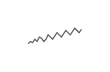
\begin{tikzpicture}[x=0.08em, y=0.08em, line width=0.4pt]
                \draw[FooterGray] (0,3) -- (1,4) -- (2,3.5) -- (3,5) -- (4,4) -- (5,6) -- (6,5.5) -- (7,4) -- (8,5) -- (9,7) -- (10,6) -- (11,5) -- (12,6.5) -- (13,8) -- (14,7) -- (15,6) -- (16,7.5) -- (17,9) -- (18,8) -- (19,7) -- (20,8.5) -- (21,10) -- (22,9) -- (23,8) -- (24,9.5);
            \end{tikzpicture}%
        }%
        \hskip0.5cm%
    }%
    \vskip6pt%
}

%=============================================================================
% PACHETE
%=============================================================================
\usepackage[utf8]{inputenc}
\usepackage[T1]{fontenc}
\usepackage{amsmath, amssymb, amsthm}
\usepackage{mathtools}
\usepackage{bm}
\usepackage{tikz}
\usetikzlibrary{arrows.meta, positioning, shapes, calc, decorations.pathreplacing, shadings}
\usepackage{booktabs}
\usepackage{multirow}
\usepackage{array}
\usepackage{graphicx}
\usepackage{hyperref}
\usepackage{colortbl}
\usepackage{pifont}
\usepackage{listings}
\lstset{language=Python, basicstyle=\ttfamily\scriptsize, keywordstyle=\color{MainBlue}\bfseries,
  commentstyle=\color{Forest}, stringstyle=\color{Crimson}, breaklines=true,
  frame=none, backgroundcolor=\color{VeryLightGray}, xleftmargin=2mm}
\hypersetup{colorlinks=true, linkcolor=MainBlue, urlcolor=MainBlue}
\graphicspath{{../../logos/}{../../charts/}{../../photos/}}
\hfuzz=5pt
\vfuzz=5pt
\hbadness=2000

%=============================================================================
% COMANDA QUANTLET
%=============================================================================
\newcommand{\quantlet}[2]{%
    \vspace{-0.25cm}%
    \hfill\href{#2}{%
        \raisebox{-0.15em}{
\includegraphics[height=0.7em]{ql_logo.png}}%
        \textcolor{MainBlue}{\tiny\ #1}%
    }\par%
}

\newcommand{\figql}[2]{%
    {\centering\href{#2}{%
        \raisebox{-0.15em}{
\includegraphics[height=0.6em]{ql_logo.png}}%
        \textcolor{MainBlue}{\tiny\ #1}%
    }\par}%
}

%=============================================================================
% PAGINA TITLU
%=============================================================================
\defbeamertemplate*{title page}{hybrid}[1][]
{
    \hfuzz=10pt%
    \vfuzz=10pt%
    \vspace{0.2cm}
    \noindent\makebox[\textwidth]{%
        \href{https://www.ase.ro}{
\includegraphics[height=0.95cm]{ase_logo.png}}\hfill%
        \href{https://theida.net}{
\includegraphics[height=0.95cm]{ida_logo.png}}\hfill%
        \href{https://blockchain-research-center.com}{
\includegraphics[height=0.95cm]{brc_logo.png}}\hfill%
        \href{https://www.ai4efin.ase.ro}{
\includegraphics[height=0.95cm]{ai4efin_logo.png}}\hfill%
        \href{https://ipe.ro/new}{
\includegraphics[height=0.95cm]{acad_logo.png}}\hfill%
        \href{https://www.digital-finance-msca.com}{
\includegraphics[height=0.95cm]{msca_logo.png}}%
    }

    \vspace{0.6cm}

    \noindent\makebox[\textwidth]{%
        \href{https://quantlet.com}{
\includegraphics[height=1.0cm]{ql_logo.png}}%
        \hfill%
        \begin{minipage}{0.78\textwidth}
            \centering
            {\LARGE\bfseries\usebeamercolor[fg]{title}\inserttitle}

            \vspace{0.3cm}

            {\usebeamerfont{subtitle}\usebeamercolor[fg]{title}\insertsubtitle}
        \end{minipage}%
        \hfill%
        \href{https://quantinar.com}{
\includegraphics[height=1.0cm]{qr_logo.png}}%
    }

    \vspace{0.6cm}

    \hspace{0.5cm}\begin{minipage}[t]{0.85\textwidth}
        \usebeamerfont{author}\insertauthor
    \end{minipage}

    \vspace{0.3cm}

    \hspace{0.5cm}\begin{minipage}[t]{0.85\textwidth}
        \raggedright\small\insertinstitute
    \end{minipage}
}

%=============================================================================
% MEDII PENTRU TEOREME
%=============================================================================
\theoremstyle{definition}
\setbeamertemplate{theorems}[numbered]
\newtheorem{defn}{Defini\c tie}
\newtheorem{thm}{Teorem\u a}
\newtheorem{prop}{Propozi\c tie}
\newtheorem{rmk}{Observa\c tie}

\newenvironment{cminipage}[1]{%
    \par\noindent\hfill\begin{minipage}{#1}\ignorespaces
}{%
    \end{minipage}\hfill\null\par
}

%=============================================================================
% COMENZI PERSONALIZATE
%=============================================================================
\newcommand{\E}{\mathbb{E}}
\newcommand{\Var}{\text{Var}}
\newcommand{\Cov}{\text{Cov}}
\newcommand{\Corr}{\text{Corr}}
\newcommand{\R}{\mathbb{R}}
\newcommand{\N}{\mathbb{N}}
\newcommand{\Z}{\mathbb{Z}}
\newcommand{\B}{\mathbf{B}}
\newcommand{\VaR}{\text{VaR}}
\newcommand{\ES}{\text{ES}}
\newcommand{\imark}{\textcolor{MainBlue}{\textbullet}}

% Indicatoare nivel academic
\newcount\slidelevelnum
\global\slidelevelnum=0
\makeatletter
\newcommand{\slidelevel}[1]{%
    \global\slidelevelnum=0%
    \def\tmp@SL{#1}\def\tmp@SLy{Y3}\def\tmp@SLm{MSc}\def\tmp@SLp{PhD}%
    \ifx\tmp@SL\tmp@SLy \global\slidelevelnum=1\fi%
    \ifx\tmp@SL\tmp@SLm \global\slidelevelnum=2\fi%
    \ifx\tmp@SL\tmp@SLp \global\slidelevelnum=3\fi%
}
\makeatother
\gdef\currentlevelcolor{FooterGray}
\newcommand{\showlevel}{%
    \ifnum\slidelevelnum=1%
        \colorbox{Forest}{\strut\textcolor{white}{\sffamily\bfseries\fontsize{8}{9}\selectfont Y3}}%
        \gdef\currentlevelcolor{Forest}%
    \fi%
    \ifnum\slidelevelnum=2%
        \colorbox{MainBlue}{\strut\textcolor{white}{\sffamily\bfseries\fontsize{8}{9}\selectfont MSc}}%
        \gdef\currentlevelcolor{MainBlue}%
    \fi%
    \ifnum\slidelevelnum=3%
        \colorbox{Crimson}{\strut\textcolor{white}{\sffamily\bfseries\fontsize{8}{9}\selectfont PhD}}%
        \gdef\currentlevelcolor{Crimson}%
    \fi%
    \ifnum\slidelevelnum=0%
        \gdef\currentlevelcolor{FooterGray}%
    \fi%
}

%=============================================================================
% INFORMATII TITLU
%=============================================================================
\title[Statistica Pie\c telor Financiare]{Statistica Pie\c telor Financiare}
\subtitle{Capitolul 11: Value-at-Risk \c si Expected Shortfall}
\author[D.T. Pele, A. Amza]{\texorpdfstring{\begin{tabular}[t]{@{}l@{}}Daniel Traian PELE \\ Antoaneta Amza\end{tabular}}{Daniel Traian PELE, Antoaneta Amza}}
\institute{Academia de Studii Economice din Bucure\c sti\\
IDA Institute Digital Assets\\
Blockchain Research Center\\
AI4EFin Artificial Intelligence for Energy Finance\\
Academia Rom\^an\u a, Institutul de Prognoz\u a Economic\u a\\
MSCA Digital Finance}
\date{}

\begin{document}

% Pagina titlu
{
\setbeamertemplate{headline}{}
\setbeamertemplate{footline}{}
\begin{frame}[noframenumbering]
    \titlepage
\end{frame}
}

%=============================================================================
% INTRO VIZUAL: ce este VaR (cartoon)
%=============================================================================
{
\setbeamertemplate{headline}{%
    \vskip10pt%
    \hbox to \paperwidth{\hskip0.5cm\hfill\textcolor{FooterGray}{\small\insertframenumber}\hskip0.5cm}%
    \vskip4pt%
    {\color{FooterGray}\hrule height 0.4pt}%
}
\slidelevel{Y3}
\begin{frame}{VaR pe \^in\c telesul tuturor}
\begin{cminipage}{0.96\textwidth}
\begin{columns}[T]
\begin{column}{0.34\textwidth}
\centering

\includegraphics[height=0.82\textheight]{intro_var.png}
\end{column}
\begin{column}{0.63\textwidth}
\vspace{0.3cm}
\begin{block}{Trei ingrediente \^in r\u aspunsul zebrei}
\begin{itemize}\setlength{\itemsep}{3pt}
    \item \textbf{Nivel de \^incredere}: ,,99\%''
    \item \textbf{Orizont}: ,,today'' (1 zi)
    \item \textbf{Pierdere}: ,,7 cm of tail''
\end{itemize}
\end{block}
\vspace{0.2cm}
\begin{exampleblock}{Traducere financiar\u a}
\begin{itemize}\setlength{\itemsep}{2pt}
    \item $\alpha = 1\%$, orizont $h = 1$ zi
    \item $\VaR_{1\%}^{1d} = $ 7 cm (echivalent monetar)
    \item \textbf{ES}: \^in cele 1\% cazuri r\u amase, c\^at pierd \emph{\^in medie}?
\end{itemize}
\end{exampleblock}
\vspace{0.1cm}
{\scriptsize\textcolor{MediumGray}{\textit{Sursa: g-square.in (2017)}}}
\end{column}
\end{columns}
\end{cminipage}
\end{frame}
}

%=============================================================================
% OBIECTIVE DE INVATARE
%=============================================================================
\slidelevel{Y3}
\begin{frame}{Obiective de \^inv\u a\c tare}
\begin{cminipage}{0.95\textwidth}
\begin{block}{La finalul acestui capitol, ve\c ti fi capabili s\u a:}
\footnotesize
\begin{enumerate}\setlength{\itemsep}{1pt}
    \item[\textcolor{MainBlue}{\textbf{1.}}] \textbf{Defini\c ti} formal VaR \c si ES
    \item[\textcolor{MainBlue}{\textbf{2.}}] \textbf{Compara\c ti} cele 4 metode standard: HS, parametric\u a (Normal\u a / Student-$t$), Monte Carlo, GARCH-VaR
    \item[\textcolor{MainBlue}{\textbf{3.}}] \textbf{Aplica\c ti} EVT-POT pentru cozi grele
    \item[\textcolor{MainBlue}{\textbf{4.}}] \textbf{Calcula\c ti} VaR/ES pe fereastr\u a glisant\u a \c si interpreta\c ti excep\c tiile realizate
    \item[\textcolor{MainBlue}{\textbf{5.}}] \textbf{Efectua\c ti} backtesting: Kupiec POF, Christoffersen IC, Basel traffic light
    \item[\textcolor{MainBlue}{\textbf{6.}}] \textbf{Backtesta\c ti} ES via Acerbi--Szekely (FRTB)
    \item[\textcolor{MainBlue}{\textbf{7.}}] \textbf{Recunoa\c ste\c ti} c\^and VaR e\c sueaz\u a \c si justifica\c ti trecerea Basel III $\to$ ES
    \item[\textcolor{MainBlue}{\textbf{8.}}] \textbf{Analiza\c ti} studii de caz: BVB (BET), Lehman 2008, scalarea pe orizonturi
\end{enumerate}
\end{block}
\end{cminipage}
\end{frame}

%=============================================================================
% NOTATII SI ACRONIME (definite inainte de prima utilizare)
%=============================================================================
\slidelevel{Y3}
\begin{frame}[shrink=18]{Nota\c tii \c si acronime (1/2): m\u asuri, metode, backtesting}
\begin{cminipage}{0.96\textwidth}
\begin{columns}[T]
\begin{column}{0.48\textwidth}
\footnotesize
\begin{block}{M\u asuri de risc}
\begin{itemize}\setlength{\itemsep}{0pt}
    \item \textbf{VaR} -- Value-at-Risk
    \item \textbf{ES} -- Expected Shortfall
    \item \textbf{CVaR} -- Conditional VaR (sinonim cu ES)
    \item \textbf{Tail-VaR} -- alt sinonim pentru ES
\end{itemize}
\end{block}
\begin{block}{Metode de estimare}
\begin{itemize}\setlength{\itemsep}{0pt}
    \item \textbf{HS} -- Historical Simulation
    \item \textbf{MC} -- Monte Carlo
    \item \textbf{GARCH} -- Generalised Autoregressive Conditional Heteroskedasticity
    \item \textbf{EVT} -- Extreme Value Theory
    \item \textbf{POT} -- Peaks Over Threshold
    \item \textbf{GPD} -- Generalised Pareto Distribution
    \item \textbf{GED} -- Generalised Error Distribution
    \item \textbf{MLE} -- Maximum Likelihood Estimation
\end{itemize}
\end{block}
\end{column}
\begin{column}{0.48\textwidth}
\footnotesize
\begin{block}{Backtesting}
\begin{itemize}\setlength{\itemsep}{0pt}
    \item \textbf{Excep\c tie} (EN: \textit{exceedance, violation, breach, failure, hit}) -- zi \^in care pierderea realizat\u a dep\u a\c se\c ste VaR-ul prognozat: $r_t < -\widehat{\VaR}_\alpha(t)$
    \item \textbf{Rata excep\c tiilor} (EN: \textit{violation rate, failure rate}) -- propor\c tia zilelor cu excep\c tie; sub model corect $\approx \alpha$
    \item \textbf{POF} -- Proportion of Failures (testul Kupiec)
    \item \textbf{IC} -- Independence Coverage (Christoffersen)
    \item \textbf{CC} -- Conditional Coverage (POF $+$ IC)
    \item \textbf{DQ} -- Dynamic Quantile (Engle--Manganelli)
    \item \textbf{ESR} -- Expected Shortfall Regression
\end{itemize}
\end{block}
\begin{block}{Statistic\u a}
\begin{itemize}\setlength{\itemsep}{0pt}
    \item \textbf{i.i.d.} -- independente \c si identic distribuite
    \item \textbf{pmf} -- probability mass function
    \item \textbf{P\&L} -- Profit and Loss (profit \c si pierdere)
    \item \textbf{CDF} -- Cumulative Distribution Function
    \item \textbf{$\chi^2$} -- distribu\c tia chi-p\u atrat
\end{itemize}
\end{block}
\end{column}
\end{columns}
\end{cminipage}
\end{frame}

\slidelevel{Y3}
\begin{frame}[shrink=15]{Nota\c tii \c si acronime (2/2): reglementare, pie\c te, evenimente}
\begin{cminipage}{0.96\textwidth}
\begin{columns}[T]
\begin{column}{0.48\textwidth}
\footnotesize
\begin{block}{Cadrul de reglementare}
\begin{itemize}\setlength{\itemsep}{0pt}
    \item \textbf{BCBS} -- Basel Committee on Banking Supervision
    \item \textbf{FRTB} -- Fundamental Review of the Trading Book
    \item \textbf{IMA} -- Internal Models Approach
    \item \textbf{CRR} -- Capital Requirements Regulation (UE)
    \item \textbf{BNR} -- Banca Na\c tional\u a a Rom\^aniei
    \item \textbf{IG} -- Investment Grade (rating creditar bun)
\end{itemize}
\end{block}
\begin{block}{Indici \c si pie\c te}
\begin{itemize}\setlength{\itemsep}{0pt}
    \item \textbf{BVB} -- Bursa de Valori Bucure\c sti
    \item \textbf{BET} -- Bucharest Exchange Trading
    \item \textbf{S\&P 500} -- Standard \& Poor's 500
    \item \textbf{DJI} -- Dow Jones Industrial Average
    \item \textbf{NASDAQ} -- Nat. Assoc. Securities Dealers
    \item \textbf{FX} -- Foreign Exchange (valutar)
\end{itemize}
\end{block}
\end{column}
\begin{column}{0.48\textwidth}
\footnotesize
\begin{block}{Evenimente \c si institu\c tii istorice}
\begin{itemize}\setlength{\itemsep}{0pt}
    \item \textbf{LTCM} -- Long-Term Capital Management (fond 1998)
    \item \textbf{AIG} -- American International Group
    \item \textbf{SVB} -- Silicon Valley Bank (criza 2023)
    \item \textbf{COVID} -- pandemia COVID-19 (martie 2020)
    \item \textbf{Lehman} -- Lehman Brothers (faliment 2008)
    \item \textbf{Dot-com} -- bula tehnologic\u a (2000--2002)
\end{itemize}
\end{block}
\end{column}
\end{columns}
\end{cminipage}
\end{frame}

%=============================================================================
% CUPRINS
%=============================================================================
{
\setbeamertemplate{headline}{%
    \vskip10pt%
    \hbox to \paperwidth{\hskip0.5cm\hfill\hskip0.5cm}%
    \vskip4pt%
    {\color{FooterGray}\hrule height 0.4pt}%
}
\begin{frame}{}
    {\color{FooterGray}\hrule height 0.4pt}
    \vspace{0.1cm}
    {\Large\textcolor{IDAred}{\textbf{Cuprins}}}
    \vspace{0.2cm}
    {\small
    \begin{columns}[T]
        \begin{column}{0.48\textwidth}
            \begin{enumerate}
                \item Motiva\c tie \c si cadru de reglementare
                \item Defini\c tia formal\u a a VaR
                \item Metode de estimare: HS, parametric, MC
                \item GARCH-VaR (condi\c tional)
                \item EVT: peaks-over-threshold (POT)
                \item Expected Shortfall (ES)
                \item M\u asuri coerente de risc (Artzner)
            \end{enumerate}
        \end{column}
        \begin{column}{0.48\textwidth}
            \begin{enumerate}\setcounter{enumi}{7}
                \item Estimare rolling
                \item Backtesting VaR (Kupiec, Christoffersen)
                \item Basel Traffic Light
                \item Backtesting ES (Acerbi--Szekely)
                \item Studii de caz: BVB, Lehman 2008
                \item Recomand\u ari practice \c si FRTB
                \item Concluzii \c si referin\c te
            \end{enumerate}
        \end{column}
    \end{columns}
    }
\end{frame}
}

%#############################################################################
\section{Motiva\c tie}
%#############################################################################

\slidelevel{Y3}
\begin{frame}{De ce avem nevoie de VaR \c si ES?}
\begin{cminipage}{0.95\textwidth}
\begin{itemize}\setlength{\itemsep}{1pt}
    \item \textbf{\^Intrebarea fundamental\u a}: \textit{,,C\^at de mult pot s\u a pierd m\^aine cu o probabilitate dat\u a?''}
    \item \textbf{Volatilitatea $\sigma$} m\u asoar\u a dispersia simetric\u a $\Rightarrow$ \textbf{nu surprinde riscul de coad\u a}
    \item \textbf{Exemplul Black Monday 1987}: $-22{,}6\%$ \^intr-o zi pentru S\&P~500
    \begin{itemize}\setlength{\itemsep}{0pt}
        \item Sub gaussianitate ($\mu = 0$, $\sigma = 1\%$): $\Pr(r \leq -22{,}6\%) \approx 10^{-115}$
    \end{itemize}
    \item \textbf{Lehman 2008}: pierderile $z$-score $> -10\sigma$ s-au repetat de 5 ori \^intr-o lun\u a
    \item \textbf{Cerin\c te de reglementare (Basel)}: capital propriu \textit{,,acoperitor''} pentru risc de pia\c t\u a
\end{itemize}
\vspace{0.15cm}
\begin{alertblock}{Concluzia}
\begin{itemize}\setlength{\itemsep}{0pt}
    \item Avem nevoie de m\u asuri de risc care surprind explicit \textbf{cozile} distribu\c tiei pierderilor
    \item \textbf{VaR} -- cuantila distribu\c tiei pierderilor
    \item \textbf{ES} -- media \^in coad\u a (peste pragul VaR)
\end{itemize}
\end{alertblock}
\end{cminipage}
\end{frame}

\slidelevel{Y3}
\begin{frame}[shrink=10]{Cadrul de reglementare: Basel I $\to$ Basel III $\to$ FRTB}
\begin{cminipage}{0.96\textwidth}
\renewcommand{\arraystretch}{1.25}
\begin{center}
\small
\begin{tabular}{lll}
\toprule
\textbf{An} & \textbf{Acord} & \textbf{Contribu\c tie cheie} \\
\midrule
1988 & Basel I & Risk-weighted assets; capital minim 8\% \\
1996 & Market Risk Amendment & \textbf{VaR 99\%, 10 zile} pentru riscul de pia\c t\u a \\
2004 & Basel II & Internal Models Approach (IMA); traffic light \\
2010--13 & Basel III & Capital + lichiditate; Stressed VaR \\
2016--19 & FRTB & \textbf{Trecere de la VaR la ES 97{,}5\%}; orizonturi diferen\c tiate \\
2023+ & Basel III final & Output floor; revizuiri IMA \\
\bottomrule
\end{tabular}
\end{center}
\vspace{0.25cm}
\begin{itemize}\setlength{\itemsep}{1pt}
    \item \textbf{De ce trecerea VaR $\to$ ES?} VaR nu e coerent\u a (non-subaditivitate) \c si nu surprinde severitatea pierderilor extreme
    \item \textbf{FRTB}: ES 97{,}5\% sub o calibrare \c stresat\u a, cu orizonturi de lichiditate (10--120 zile) per factor de risc
\end{itemize}
\end{cminipage}
\end{frame}

\slidelevel{Y3}
\begin{frame}{De la cuantil\u a la VaR --- intui\c tia vizual\u a}
\begin{cminipage}{0.96\textwidth}
\begin{columns}[T]
\begin{column}{0.50\textwidth}
\begin{itemize}\setlength{\itemsep}{1pt}
    \item Fie $X$ rentabilitatea (sau P\&L) zilnic\u a a portofoliului
    \item Cuantila de ordin $\alpha$ a lui $X$:
    \[
        q_\alpha = F_X^{-1}(\alpha) = \inf\{x : F_X(x) \geq \alpha\}
    \]
    \item Pentru $\alpha = 5\%$: $q_{0{,}05}$ este dep\u a\c sit (la sc\u adere) doar 5\% din timp
    \item \textbf{VaR} este \textbf{magnitudinea pierderii} corespunz\u atoare (semn schimbat):
    \[
        \boxed{\VaR_\alpha = -q_\alpha = -F_X^{-1}(\alpha)}
    \]
    \item Conven\c tia: \textit{,,VaR 5\%''} $\equiv$ $\alpha = 0{,}05$ (pierdere dep\u a\c sit\u a cu probabilitate 5\%)
\end{itemize}
\end{column}
\begin{column}{0.46\textwidth}
\centering
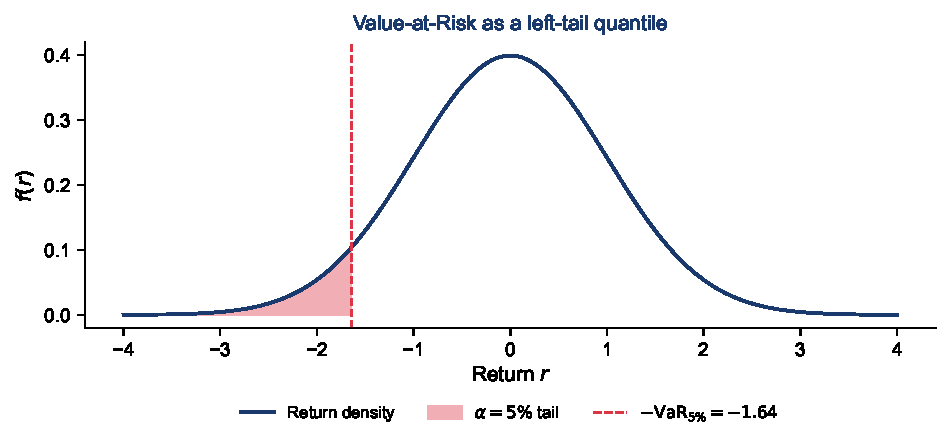
\includegraphics[width=\linewidth]{ch11_var_concept.pdf}
\figql{SFM\_ch11\_var\_concept}{https://github.com/danpele/SFM/tree/main/Quantlets/Ch_11/SFM_ch11_var_concept}
\end{column}
\end{columns}
\end{cminipage}
\end{frame}

\slidelevel{Y3}
\begin{frame}[shrink=10]{Scurt\u a istorie a VaR}
\begin{cminipage}{0.96\textwidth}
\renewcommand{\arraystretch}{1.2}
\begin{center}
\small
\begin{tabular}{lll}
\toprule
\textbf{An} & \textbf{Eveniment / actor} & \textbf{Contribu\c tie} \\
\midrule
1922 & US Commerce Dept.\ & Cerin\c te capital pe baz\u a probabilistic\u a \\
1952 & H. Markowitz & Frontiera medie--varian\c t\u a (CAPM) \\
1963 & B. Mandelbrot & Pre\c turi bumbac: cozi grele $\Rightarrow$ VaR Normal inadecvat \\
1973 & Black-Scholes & Op\c tiuni $\Rightarrow$ nevoia VaR neliniar \\
1993 & G30 report & Recomandare oficial\u a: m\u asuri de risc \^in firmele financiare \\
1994 & \textbf{JP Morgan RiskMetrics} & Publicarea metodologiei VaR Normal \\
1996 & Basel MRA & VaR 99\% 10-zile devine cerin\c t\u a regulator \\
1998 & LTCM collapse & E\c sec VaR: 4 SD ,,o-dat\u a-la-mileniu'' \^in 6 luni \\
1999 & Artzner et al. & Axiomele coeren\c tei; VaR non-subaditiv \\
2002 & Acerbi--Tasche & ES coerent\u a; fundamentul matematic FRTB \\
2008 & Lehman crisis & E\c sec sistemic VaR; reform\u a Basel III \\
2016 & BCBS FRTB & ES 97,5\% \^inlocuie\c ste VaR \\
\bottomrule
\end{tabular}
\end{center}
\end{cminipage}
\end{frame}

\slidelevel{MSc}
\begin{frame}{Pierderi celebre cuantificate (failure cases)}
\begin{cminipage}{0.96\textwidth}
\renewcommand{\arraystretch}{1.25}
\begin{center}
\small
\begin{tabular}{lcc l}
\toprule
\textbf{Eveniment} & \textbf{Pierdere} & \textbf{An} & \textbf{Cauza prim\u a} \\
\midrule
Barings Bank & \$1{,}3 mld & 1995 & Trader fraud (Nick Leeson); VaR ne-monitorizat \\
LTCM & \$4{,}6 mld & 1998 & Modele Normal; lichiditate ignorat\u a \\
Soci\'et\'e G\'en\'erale & EUR4{,}9 mld & 2008 & Fraud trader; VaR by-passed \\
JP Morgan ,,London Whale'' & \$6{,}2 mld & 2012 & Model VaR manipulat \\
Archegos & \$10 mld & 2021 & Family office; leverage 5x; VaR cumulativ ignorat \\
SVB & \$15 mld & 2023 & Risc duration; VaR rate dob\^and\u a inadecvat \\
FTX collapse & \$8 mld & 2022 & Crypto contagion; VaR cripto subestimat \\
\bottomrule
\end{tabular}
\end{center}
\vspace{0.2cm}
\begin{alertblock}{Pattern}
\begin{itemize}\setlength{\itemsep}{0pt}
    \item \^In toate cazurile: \textbf{VaR raportat $\ll$ pierderea realizat\u a}
    \item Cauze comune: model misspecification, fraud, lichiditate ignorat\u a, governance
\end{itemize}
\end{alertblock}
\end{cminipage}
\end{frame}

\slidelevel{MSc}
\begin{frame}[shrink=5]{VaR \^in regimuri reglementare globale}
\begin{cminipage}{0.96\textwidth}
\renewcommand{\arraystretch}{1.2}
\begin{center}
\footnotesize
\begin{tabular}{l l l l l}
\toprule
\textbf{Cadru} & \textbf{Sector} & \textbf{Statistic\u a} & \textbf{Nivel} & \textbf{Orizont} \\
\midrule
Basel III (BCBS) & Banc\u a -- trading & VaR + Stressed VaR & 99\% & 10 zile \\
FRTB (BCBS 2016+) & Banc\u a -- trading & \textbf{Expected Shortfall} & 97,5\% & 10--120 zile \\
Solvency II (EIOPA) & Asigur\u ari & VaR & 99,5\% & 1 an \\
CCAR / DFAST (Fed) & Banc\u a US -- stress & Scenario PV & ,,severely adverse'' & 9 trimestre \\
ICAAP (banc\u a intern) & Banc\u a -- intern & VaR + ES & 99,9\% & 1 an \\
MiFID II & Investitori retail & VaR (PRIIPs) & 97,5\% & holding period \\
\bottomrule
\end{tabular}
\end{center}
\vspace{0.15cm}
\begin{itemize}\setlength{\itemsep}{0pt}
    \item \textbf{Observa\c tii}: cuantil\u a mai mic\u a $\Rightarrow$ orizont mai lung
    \item Asigur\u arile folosesc cuantile mai extreme (99,5\%) pe orizonturi anuale
    \item Bancile US complementeaz\u a VaR cu \textbf{stress testing scenario-based} (CCAR)
    \item Rom\^ania: BNR aplic\u a direct CRR3 (Basel III final, transpunere UE)
\end{itemize}
\end{cminipage}
\end{frame}

%#############################################################################
\section{Defini\c tia formal\u a a VaR}
%#############################################################################

\slidelevel{MSc}
\begin{frame}[shrink=20]{Defini\c tia formal\u a}
\begin{cminipage}{0.95\textwidth}
\begin{defn}[Value-at-Risk]
\begin{itemize}\setlength{\itemsep}{0pt}
    \item Nota\c tii: $L = -X$ pierderea la orizont $h$, $F_L$ func\c tia de reparti\c tie
    \item Pentru $\alpha \in (0,1)$:
    \[
        \VaR_\alpha(L) = \inf\{\ell \in \R : \Pr(L > \ell) \leq \alpha\} = F_L^{-1}(1-\alpha)
    \]
    \item Echivalent pe rentabilitatea $X$: $\VaR_\alpha = -F_X^{-1}(\alpha)$
\end{itemize}
\end{defn}

\vspace{0.15cm}

\begin{block}{Trei elemente esen\c tiale specific\u ari}
\begin{enumerate}\setlength{\itemsep}{1pt}
    \item \textbf{Nivelul de \^incredere} $1-\alpha$: 95\%, 99\%, 99{,}9\%
    \item \textbf{Orizontul temporal} $h$: 1 zi (trading book), 10 zile (Basel), 1 an (credit)
    \item \textbf{Distribu\c tia de referin\c t\u a}: empiric\u a, Normal\u a, Student-$t$, mixt\u a, GARCH\dots
\end{enumerate}
\end{block}

\vspace{0.1cm}

\begin{alertblock}{Conven\c tie de semn}
\begin{itemize}\setlength{\itemsep}{0pt}
    \item $\VaR_\alpha > 0$: m\u arime de pierdere pozitiv\u a (e.g., $\VaR_{1\%} = 35.000$ EUR)
    \item Cu probabilitatea $1-\alpha$, pierderea \textbf{nu va dep\u a\c si} $\VaR_\alpha$
\end{itemize}
\end{alertblock}
\end{cminipage}
\end{frame}

\slidelevel{Y3}
\begin{frame}[shrink=8]{Exemplul canonic: banc\u a cu portofoliu de 1M\$}
\begin{cminipage}{0.95\textwidth}
\begin{itemize}\setlength{\itemsep}{1pt}
    \item Portofoliu $V = 1.000.000\$$, randament zilnic $r \sim \mathcal{N}(\mu, \sigma^2)$ cu $\mu = 0$, $\sigma = 1{,}5\%$
    \item Sub normalitate:
    \[
        \VaR_\alpha = -V \cdot (\mu + \sigma z_\alpha), \quad z_\alpha = \Phi^{-1}(\alpha)
    \]
    \item \textbf{Trei niveluri standard}:
\end{itemize}
\vspace{0.1cm}
\begin{center}
\renewcommand{\arraystretch}{1.2}
\small
\begin{tabular}{ccccc}
\toprule
\textbf{Nivel} & $\alpha$ & $z_\alpha$ & \textbf{VaR zilnic\u a} & \textbf{VaR 10-day} ($\sqrt{10}$) \\
\midrule
95\% & 0{,}05  & $-1{,}645$ & \$24.675 & \$78.020 \\
99\% & 0{,}01  & $-2{,}326$ & \$34.890 & \$110.327 \\
99{,}9\% & 0{,}001 & $-3{,}090$ & \$46.350 & \$146.572 \\
\bottomrule
\end{tabular}
\end{center}
\vspace{0.15cm}
\begin{exampleblock}{Interpretare}
\begin{itemize}\setlength{\itemsep}{0pt}
    \item Cu probabilitatea 99\%, banca nu va pierde mai mult de \$34.890 \^intr-o singur\u a zi de tranzac\c tionare
    \item Echivalent: ne a\c stept\u am la $\approx 2{,}5$ \textbf{excep\c tii} (EN: \textit{failures/exceedances}) pe an (250 zile lucr\u atoare $\times$ 1\%)
\end{itemize}
\end{exampleblock}
\end{cminipage}
\end{frame}

\slidelevel{MSc}
\begin{frame}{Scalarea pe orizont: regula $\sqrt{T}$ \c si capcanele ei}
\begin{cminipage}{0.96\textwidth}
\begin{columns}[T]
\begin{column}{0.50\textwidth}
\begin{itemize}\setlength{\itemsep}{1pt}
    \item Sub \textbf{normalitate \c si i.i.d.}, VaR scaleaz\u a cu $\sqrt{T}$:
    \[
        \VaR_\alpha^{(T)} = \sqrt{T} \cdot \VaR_\alpha^{(1)}
    \]
    \item \textbf{Regulatorul Basel} cere VaR pe 10 zile: practic se scaleaz\u a VaR-ul de 1 zi cu $\sqrt{10}$
    \item \textbf{Problem\u a}: regula $\sqrt{T}$ \textbf{subestimeaz\u a} VaR atunci c\^and randamentele au \textbf{cozi grele} sau \textbf{autocorela\c tie}
    \item \textbf{Diebold et al. (1997)}: ,,square-root rule is dangerous''
\end{itemize}
\end{column}
\begin{column}{0.46\textwidth}
\centering
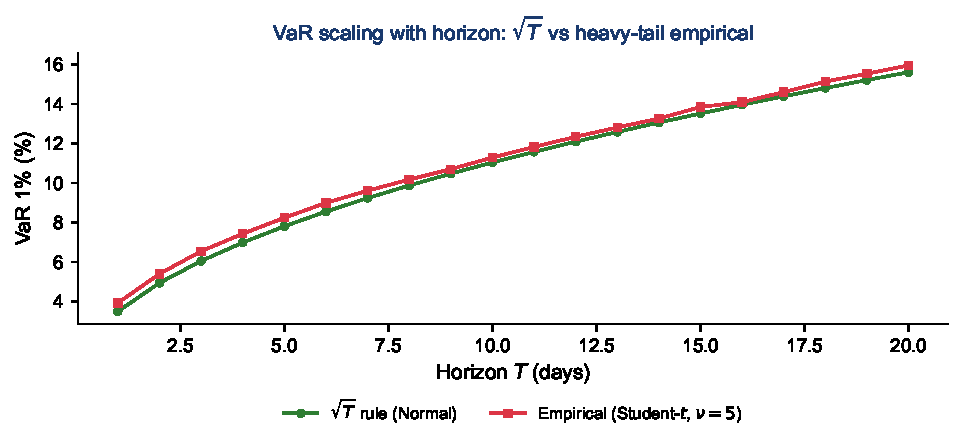
\includegraphics[width=\linewidth]{ch11_var_horizons.pdf}\\[2pt]
{\scriptsize\textcolor{MediumGray}{\textit{Regula $\sqrt{T}$ vs.\ VaR empiric sub Student-$t$ cu $\nu=5$. Diferen\c ta cre\c ste cu orizontul.}}}
\figql{SFM\_ch11\_var\_horizons}{https://github.com/danpele/SFM/tree/main/Quantlets/Ch_11/SFM_ch11_var_horizons}
\end{column}
\end{columns}
\end{cminipage}
\end{frame}

\slidelevel{MSc}
\begin{frame}{Critica fundamental\u a: VaR nu este subaditiv}
\begin{cminipage}{0.96\textwidth}
\begin{columns}[T]
\begin{column}{0.48\textwidth}
\begin{itemize}\setlength{\itemsep}{1pt}
    \item \textbf{Subaditivitate}: $\rho(X+Y) \leq \rho(X) + \rho(Y)$
    \item Echivalent: \textbf{diversificarea nu cre\c ste riscul}
    \item \textbf{Contraexemplu (Embrechts)}: dou\u a obliga\c tiuni cu default rar \c si independent, $\Pr(\text{default}) = 4\%$, pierdere 100~EUR
    \item Pentru fiecare obliga\c tiune: $\VaR_{5\%} = 0$ (4\% < 5\%)
    \item Portofoliul $X_1 + X_2$: $\Pr(\text{cel pu\c tin un default}) = 7{,}84\%$
    \item Deci $\VaR_{5\%}(X_1 + X_2) = 100 > 0 + 0$ \quad $\Rightarrow$ \textbf{VaR e\c sueaz\u a subaditivitatea}
    \item \textbf{Concluzie}: VaR nu este o m\u asur\u a coerent\u a de risc
\end{itemize}
\end{column}
\begin{column}{0.50\textwidth}
\centering
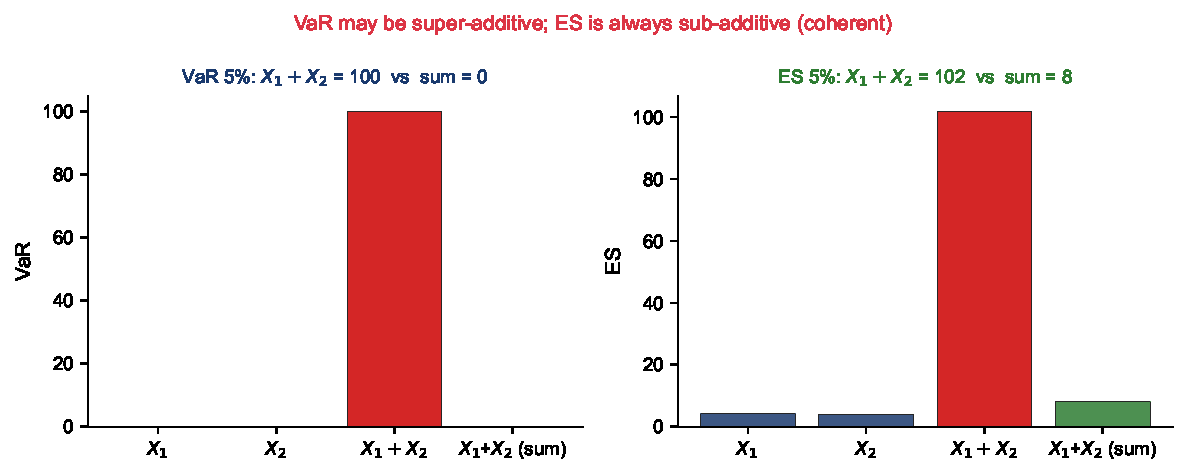
\includegraphics[width=\linewidth]{ch11_subadditivity.pdf}\\[2pt]
{\scriptsize\textcolor{MediumGray}{\textit{VaR-ul portofoliului dep\u a\c se\c ste suma VaR-urilor individuale (failure). ES respect\u a subaditivitatea.}}}
\figql{SFM\_ch11\_subadditivity}{https://github.com/danpele/SFM/tree/main/Quantlets/Ch_11/SFM_ch11_subadditivity}
\end{column}
\end{columns}
\end{cminipage}
\end{frame}

%#############################################################################
\section{Metode de estimare: HS, parametric, MC}
%#############################################################################

\slidelevel{Y3}
\begin{frame}[shrink=10]{Cele 4 metode standard de estimare}
\begin{cminipage}{0.95\textwidth}
\renewcommand{\arraystretch}{1.25}
\begin{center}
\footnotesize
\begin{tabular}{llll}
\toprule
\textbf{Metoda} & \textbf{Idee principal\u a} & \textbf{Distribu\c tie} & \textbf{Limitare} \\
\midrule
Simulare istoric\u a (HS) & cuantil\u a empiric\u a rolling & non-parametric\u a & ,,ghost effects'' \\
Parametric\u a Normal\u a & $\VaR = -(\mu + \sigma z_\alpha)$ & $\mathcal{N}(\mu, \sigma^2)$ & subestimeaz\u a cozile \\
Parametric\u a Student-$t$ & cuantil\u a $t_\nu$ scalat\u a & $t_\nu$ & estimarea $\nu$ \\
Monte Carlo & simulare scenarii & orice & cost computa\c tional \\
GARCH-VaR & $\VaR_t = -(\mu_t + \sigma_t z_\alpha)$ & condi\c tional\u a & acurate\c tea GARCH \\
EVT (POT) & GPD pe excese & extrem\u a $\Rightarrow$ GPD & alegerea pragului $u$ \\
\bottomrule
\end{tabular}
\end{center}
\vspace{0.2cm}
\begin{block}{Recomandare general\u a}
\begin{itemize}\setlength{\itemsep}{0pt}
    \item \textbf{HS}: simpl\u a, robust\u a, recomandat\u a ca \textit{benchmark}
    \item \textbf{GARCH-VaR}: cea mai bun\u a pentru regimuri volatile (criz\u a)
    \item \textbf{EVT}: cea mai bun\u a pentru cuantile extreme ($\alpha \leq 1\%$)
\end{itemize}
\end{block}
\end{cminipage}
\end{frame}

\slidelevel{Y3}
\begin{frame}{Metoda 1: Simulare istoric\u a (HS) -- algoritm}
\begin{cminipage}{0.96\textwidth}
\begin{block}{Algoritm}
\begin{enumerate}\setlength{\itemsep}{1pt}
    \item Alege o fereastr\u a $\{r_{t-W+1}, \ldots, r_t\}$, e.g., $W = 250$ zile
    \item Sorteaz\u a randamentele cresc\u ator: $r_{(1)} \leq r_{(2)} \leq \cdots \leq r_{(W)}$
    \item Cuantila empiric\u a: $\widehat{\VaR}_\alpha = -r_{(\lceil \alpha W\rceil)}$
    \item Expected Shortfall: $\widehat{\ES}_\alpha = -\frac{1}{\lceil\alpha W\rceil}\sum_{i=1}^{\lceil\alpha W\rceil} r_{(i)}$
\end{enumerate}
\end{block}
\vspace{0.2cm}
\begin{center}
\quantlet{SFM\_ch11\_method\_hs}{https://github.com/danpele/SFM/tree/main/Quantlets/Ch_11/SFM_ch11_method_hs}
\end{center}
\end{cminipage}
\end{frame}

\slidelevel{Y3}
\begin{frame}{HS -- avantaje \c si dezavantaje}
\begin{cminipage}{0.96\textwidth}
\begin{columns}[T]
\begin{column}{0.49\textwidth}
\begin{exampleblock}{Avantaje}
\begin{itemize}\setlength{\itemsep}{1pt}
    \item Nu necesit\u a ipoteze distribu\c tionale
    \item Surprinde cozi grele prezente \^in fereastr\u a
    \item U\c sor de implementat \c si explicat
    \item Robust\u a la valori extreme \textbf{deja observate}
\end{itemize}
\end{exampleblock}
\end{column}
\begin{column}{0.49\textwidth}
\begin{alertblock}{Dezavantaje}
\begin{itemize}\setlength{\itemsep}{1pt}
    \item \textbf{Ghost effect}: pierdere mare r\u am\^ane \^in VaR exact $W$ zile
    \item Adaptare lent\u a la schimb\u ari de regim
    \item Subestimeaz\u a cuantile $< 1/W$ (e.g., $\alpha = 0{,}1\%$ cu $W = 250$ imposibil)
    \item Tratament egal al observa\c tiilor (nu pondereaz\u a recente)
\end{itemize}
\end{alertblock}
\end{column}
\end{columns}
\end{cminipage}
\end{frame}

\slidelevel{Y3}
\begin{frame}[shrink=15]{HS -- exemplu numeric \c si vizualizare}
\begin{cminipage}{0.96\textwidth}
\begin{columns}[T]
\begin{column}{0.42\textwidth}
\begin{exampleblock}{Exemplu: fereastra de 250 zile}
\begin{itemize}\setlength{\itemsep}{0pt}
    \item 250 randamente zilnice GARCH-$t$ simulate
    \item $\alpha = 5\% \Rightarrow$ cea de-a $\lceil 0{,}05 \cdot 250\rceil = 13$-a observa\c tie sortat\u a
    \item $\widehat{\VaR}_{5\%} = -r_{(13)} \approx 1{,}19\%$
    \item $\widehat{\ES}_{5\%} = -\overline{r_{(1)}, \ldots, r_{(13)}} \approx 1{,}65\%$
    \item Pe portofoliu 1M EUR: $\widehat{\VaR} = 11.900$ EUR, $\widehat{\ES} = 16.500$ EUR
\end{itemize}
\end{exampleblock}
\begin{block}{Interpretare}
\begin{itemize}\setlength{\itemsep}{0pt}
    \item Cu probabilitatea 95\%, pierderea nu va dep\u a\c si 11.900 EUR
    \item Dat fiind c\u a am dep\u a\c sit acest prag, pierderea medie a\c steptat\u a este 16.500 EUR
\end{itemize}
\end{block}
\end{column}
\begin{column}{0.56\textwidth}
\centering
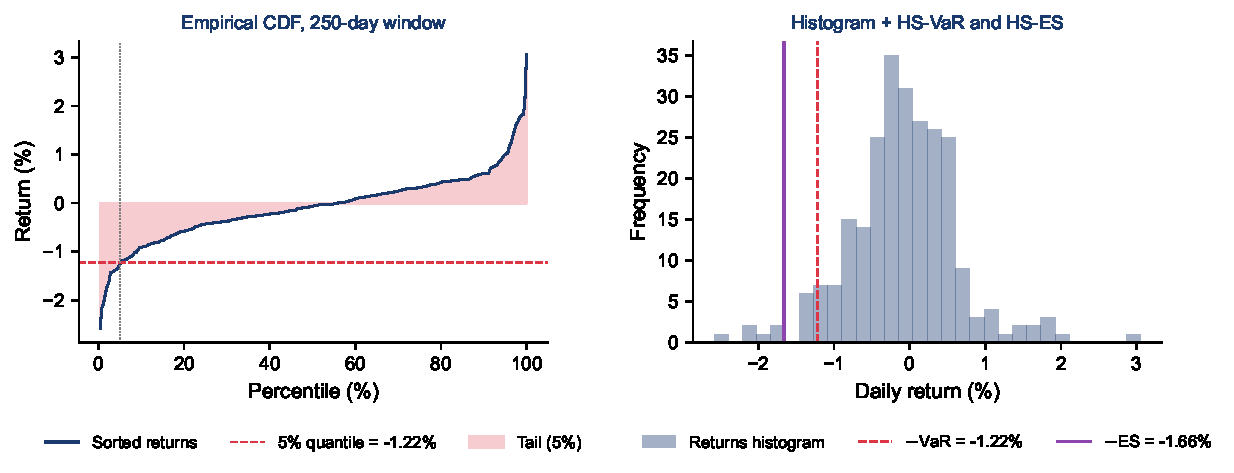
\includegraphics[width=\linewidth]{ch11_method_hs.pdf}\\[1pt]
{\scriptsize\textcolor{MediumGray}{\textit{St\^anga: CDF empiric\u a a celor 250 randamente. Dreapta: histogram cu VaR \c si ES marcate.}}}
\figql{SFM\_ch11\_method\_hs}{https://github.com/danpele/SFM/tree/main/Quantlets/Ch_11/SFM_ch11_method_hs}
\end{column}
\end{columns}
\end{cminipage}
\end{frame}

\slidelevel{Y3}
\begin{frame}[shrink=15]{Metoda 2: Parametric\u a Normal\u a -- formule}
\begin{cminipage}{0.96\textwidth}
\begin{block}{Formula \^inchis\u a}
\begin{itemize}\setlength{\itemsep}{0pt}
    \item Ipoteza: $r \sim \mathcal{N}(\mu, \sigma^2)$
    \item $\VaR_\alpha = -(\mu + \sigma z_\alpha)$, cu $z_\alpha = \Phi^{-1}(\alpha)$
    \item $\ES_\alpha = -\mu + \sigma \cdot \phi(z_\alpha)/\alpha$, unde $\phi$ este densitatea $\mathcal{N}(0,1)$
\end{itemize}
\end{block}

\begin{block}{Portofoliu multivariat}
\begin{itemize}\setlength{\itemsep}{0pt}
    \item Notatii: $\bm w$ ponderi, $\bm \Sigma$ matricea de covarian\c t\u a, $V$ valoarea portofoliului
    \item Volatilitatea portofoliului: $\sigma_p = \sqrt{\bm w^\top \bm \Sigma \bm w}$
    \item $\VaR_\alpha^{port} = -V \cdot (\bm w^\top \bm\mu + \sigma_p z_\alpha)$
\end{itemize}
\end{block}

\begin{alertblock}{Limit\u ari}
\begin{itemize}\setlength{\itemsep}{0pt}
    \item Subestimeaz\u a sistematic VaR-ul \^in cozi (Normalitate $\Rightarrow$ cozi sub\c tiri)
    \item Pentru $\alpha = 0{,}1\%$: subestimare de 60--150\% (Student-$t$/stable)
    \item Ignor\u a asimetria \c si volatility clustering (clustering de volatilitate)
\end{itemize}
\end{alertblock}
\end{cminipage}
\end{frame}

\slidelevel{Y3}
\begin{frame}[shrink=15]{Normal\u a -- exemplu numeric \c si vizualizare}
\begin{cminipage}{0.96\textwidth}
\begin{columns}[T]
\begin{column}{0.42\textwidth}
\begin{exampleblock}{Exemplu: pe 250 zile, $\hat\mu \approx 0$, $\hat\sigma \approx 1{,}5\%$}
\begin{itemize}\setlength{\itemsep}{0pt}
    \item $\VaR_{5\%} = 1{,}5\% \cdot 1{,}645 = 2{,}47\%$
    \item $\ES_{5\%}  = 1{,}5\% \cdot \phi(-1{,}645)/0{,}05 = 3{,}09\%$
    \item $\VaR_{1\%} = 1{,}5\% \cdot 2{,}326 = 3{,}49\%$
    \item $\ES_{1\%}  = 1{,}5\% \cdot 2{,}665 = 4{,}00\%$
    \item $\VaR_{0{,}1\%} = 1{,}5\% \cdot 3{,}090 = 4{,}64\%$
\end{itemize}
\end{exampleblock}
\begin{block}{Pe portofoliu 1M EUR}
\begin{itemize}\setlength{\itemsep}{0pt}
    \item $\VaR_{1\%} \approx$ 34.890 EUR
    \item $\ES_{1\%}  \approx$ 40.000 EUR
    \item Capital Basel = $3 \cdot \VaR_{1\%}^{10d}$ $\approx$ 331.000 EUR
\end{itemize}
\end{block}
\end{column}
\begin{column}{0.56\textwidth}
\centering
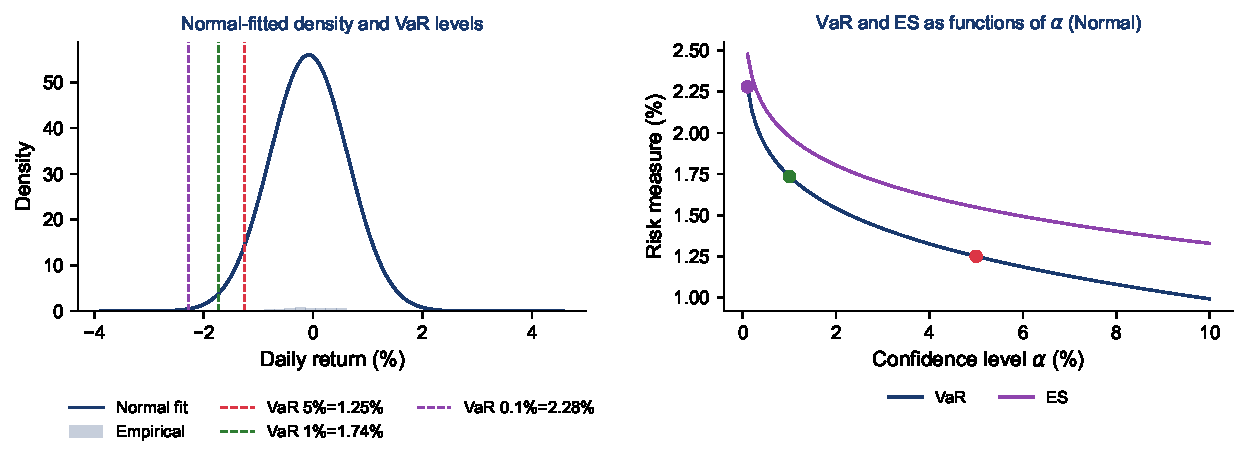
\includegraphics[width=\linewidth]{ch11_method_normal.pdf}\\[1pt]
{\scriptsize\textcolor{MediumGray}{\textit{St\^anga: densitatea Normal\u a estimat\u a cu trei niveluri VaR. Dreapta: VaR \c si ES ca func\c tii continue de $\alpha$.}}}
\figql{SFM\_ch11\_method\_normal}{https://github.com/danpele/SFM/tree/main/Quantlets/Ch_11/SFM_ch11_method_normal}
\end{column}
\end{columns}
\end{cminipage}
\end{frame}

\slidelevel{MSc}
\begin{frame}{Metoda 3: Parametric\u a Student-$t$ (cozi grele)}
\begin{cminipage}{0.96\textwidth}
\begin{itemize}\setlength{\itemsep}{1pt}
    \item Ipoteza: $r = \mu + \sigma\cdot T_\nu$ cu $T_\nu$ standardizat $\sim t(\nu)$ ($\nu > 2$)
    \item Formula \^inchis\u a:
    \[
        \VaR_\alpha = -\Big(\mu + \sigma \sqrt{\tfrac{\nu-2}{\nu}}\, t_\nu^{-1}(\alpha)\Big)
    \]
    \[
        \ES_\alpha = -\mu + \sigma \sqrt{\tfrac{\nu-2}{\nu}} \cdot \frac{f_{\nu}(t_\nu^{-1}(\alpha))}{\alpha} \cdot \frac{\nu + (t_\nu^{-1}(\alpha))^2}{\nu - 1}
    \]
    \item \textbf{Estimare}: $\hat\nu$ prin MLE (Maximum Likelihood Estimation; vezi cap. 5)
    \item \textbf{Empiric}: $\nu \in [4, 8]$ pentru indici de ac\c tiuni; $\nu \in [3, 5]$ pentru cripto
    \item \textbf{Avantaj}: surprinde leptokurtoza, men\c tin\^and forma analitic\u a
    \item \textbf{Dezavantaj}: simetric\u a; pentru asimetrie folosi\c ti skew-$t$ sau distribu\c tii stabile
\end{itemize}
\vspace{0.1cm}
\begin{exampleblock}{Regula degetului}
\begin{itemize}\setlength{\itemsep}{0pt}
    \item La $\alpha = 1\%$: $\VaR^{t_5} \approx 1{,}25 \times \VaR^{N}$
    \item La $\alpha = 0{,}1\%$: $\VaR^{t_5} \approx 1{,}65 \times \VaR^{N}$
\end{itemize}
\end{exampleblock}
\end{cminipage}
\end{frame}

\slidelevel{MSc}
\begin{frame}[shrink=15]{Student-$t$ -- exemplu numeric \c si vizualizare}
\begin{cminipage}{0.96\textwidth}
\begin{columns}[T]
\begin{column}{0.42\textwidth}
\begin{exampleblock}{Exemplu: 1000 randamente GARCH-$t$, MLE $\hat\nu = 5{,}4$}
\begin{itemize}\setlength{\itemsep}{0pt}
    \item $\hat\mu \approx 0$, $\hat\sigma_{eff} \approx 0{,}74\%$ (din MLE)
    \item $\VaR^{N}_{1\%} = 1{,}73\%$ \quad vs.\ \quad $\VaR^{t}_{1\%} = 2{,}03\%$ (+17{,}3\%)
    \item $\ES^{t}_{1\%}  = 2{,}71\%$
    \item $\VaR^{N}_{0{,}1\%} = 2{,}29\%$ \quad vs.\ \quad $\VaR^{t}_{0{,}1\%} = 3{,}69\%$ (+61\%)
\end{itemize}
\end{exampleblock}
\begin{alertblock}{Implica\c tii}
\begin{itemize}\setlength{\itemsep}{0pt}
    \item Diferen\c ta cre\c ste cu $\alpha$ mai mic
    \item La $\alpha = 0{,}1\%$: Student-$t$ cere capital cu 60--80\% mai mare
\end{itemize}
\end{alertblock}
\end{column}
\begin{column}{0.56\textwidth}
\centering
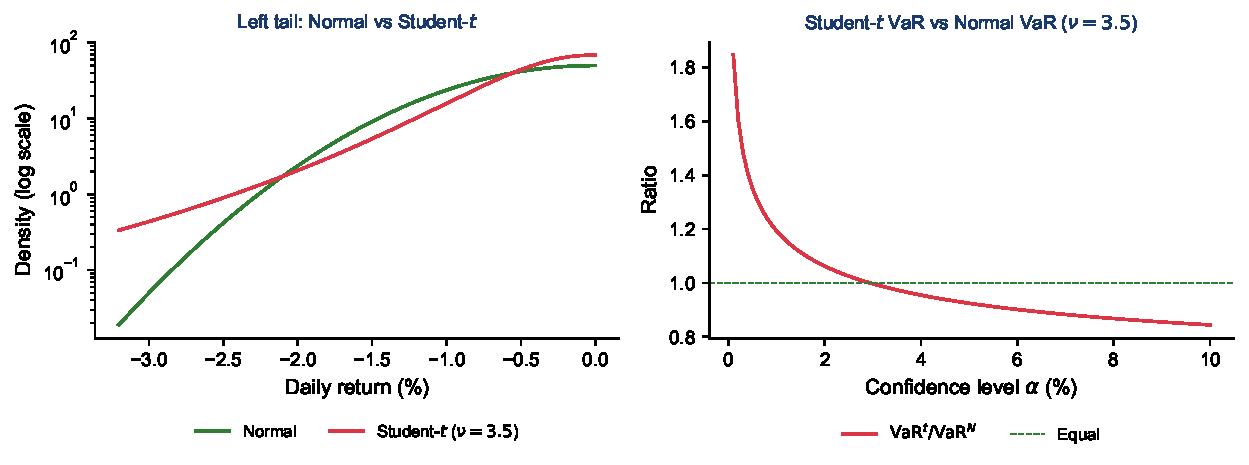
\includegraphics[width=\linewidth]{ch11_method_student_t.pdf}\\[1pt]
{\scriptsize\textcolor{MediumGray}{\textit{St\^anga: coada st\^ang\u a a densit\u a\c tilor pe scal\u a log. Dreapta: raportul $\VaR^{t}/\VaR^{N}$ \^in func\c tie de $\alpha$.}}}
\figql{SFM\_ch11\_method\_student\_t}{https://github.com/danpele/SFM/tree/main/Quantlets/Ch_11/SFM_ch11_method_student_t}
\end{column}
\end{columns}
\end{cminipage}
\end{frame}

\slidelevel{Y3}
\begin{frame}[shrink=15]{Metoda 4: Monte Carlo (MC) -- algoritm}
\begin{cminipage}{0.96\textwidth}
\begin{block}{Algoritm}
\begin{enumerate}\setlength{\itemsep}{0pt}
    \item Specific\u a un model pentru randamente (Normal, $t$, GARCH, mixt\dots)
    \item Genereaz\u a $M$ traiectorii (e.g., $M = 100.000$)
    \item Evalueaz\u a P\&L-ul (Profit and Loss) portofoliului pe fiecare scenariu
    \item Calculeaz\u a cuantila empiric\u a a P\&L-ului simulat
\end{enumerate}
\end{block}

\begin{columns}[T]
\begin{column}{0.49\textwidth}
\begin{exampleblock}{Avantaje}
\begin{itemize}\setlength{\itemsep}{0pt}
    \item Flexibilitate pentru produse \textbf{neliniare} (op\c tiuni, exotice)
    \item Modele complexe (jump-diffusion, regime-switching)
    \item Permite stresare explicit\u a a scenariilor
\end{itemize}
\end{exampleblock}
\end{column}
\begin{column}{0.49\textwidth}
\begin{alertblock}{Dezavantaje}
\begin{itemize}\setlength{\itemsep}{0pt}
    \item Cost computa\c tional ridicat
    \item Eroare Monte Carlo: $\propto 1/\sqrt{M}$
    \item Depinde de \textbf{model risk} (modelul ales)
\end{itemize}
\end{alertblock}
\end{column}
\end{columns}

\vspace{0.1cm}
\begin{alertblock}{Variance reduction}
\begin{itemize}\setlength{\itemsep}{0pt}
    \item La cuantile extreme ($\alpha < 1\%$), eroarea MC cre\c ste considerabil
    \item Folosi\c ti \textbf{importance sampling} sau \textbf{stratified sampling}
    \item Acestea reduc semnificativ $M$ necesar pentru aceea\c si precizie
\end{itemize}
\end{alertblock}
\end{cminipage}
\end{frame}

\slidelevel{Y3}
\begin{frame}[shrink=15]{Monte Carlo -- exemplu numeric \c si vizualizare}
\begin{cminipage}{0.96\textwidth}
\begin{columns}[T]
\begin{column}{0.42\textwidth}
\begin{exampleblock}{Exemplu: portofoliu 100 EUR, orizont 10 zile}
\begin{itemize}\setlength{\itemsep}{0pt}
    \item Model: $\Delta\ln P_t \sim \mathcal{N}(\mu - \sigma^2/2,\, \sigma^2)$, $\mu = 0{,}03\%$, $\sigma = 1{,}5\%$
    \item Setup: $M = 50.000$ traiectorii, $h = 10$ zile
    \item P\&L: $100 \cdot (\exp(\sum_{t=1}^{10} \Delta\ln P_t) - 1)$
    \item $\widehat{\VaR}^{MC}_{5\%}$ = cuantila 5\% a P\&L simulat $\approx 7{,}73$
    \item $\widehat{\ES}^{MC}_{5\%} \approx 9{,}77$
    \item Eroare standard cuantila 5\%: $\approx 0{,}07$ ($\propto 1/\sqrt{M\alpha(1-\alpha)}$)
    \item Pentru $\alpha = 0{,}1\%$, $M = 50.000$ insuficient $\Rightarrow$ importance sampling
\end{itemize}
\end{exampleblock}
\end{column}
\begin{column}{0.56\textwidth}
\centering
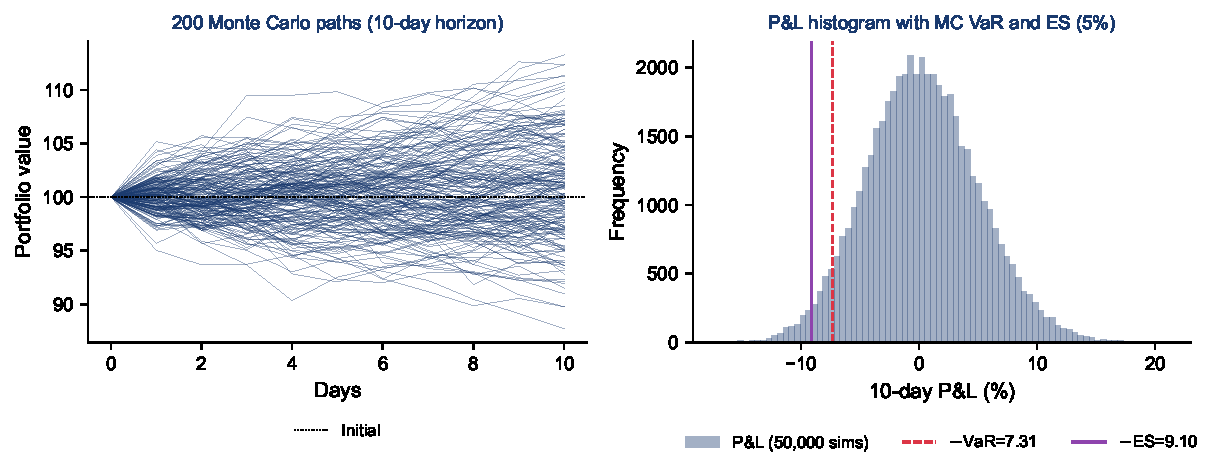
\includegraphics[width=\linewidth]{ch11_method_mc.pdf}\\[1pt]
{\scriptsize\textcolor{MediumGray}{\textit{St\^anga: 200 traiectorii MC ale valorii portofoliului. Dreapta: histograma P\&L pe 10 zile cu VaR \c si ES.}}}
\figql{SFM\_ch11\_method\_mc}{https://github.com/danpele/SFM/tree/main/Quantlets/Ch_11/SFM_ch11_method_mc}
\end{column}
\end{columns}
\end{cminipage}
\end{frame}

\slidelevel{MSc}
\begin{frame}{Compara\c tia celor patru metode pe acelea\c si date}
\begin{cminipage}{0.96\textwidth}
\begin{columns}[T]
\begin{column}{0.55\textwidth}
\begin{itemize}\setlength{\itemsep}{1pt}
    \item Date: 2500 randamente zilnice simulate GARCH(1,1)-$t_6$
    \item Toate cele 4 metode aplicate la $\alpha = 5\%$ pe \^intregul e\c santion
    \item \textbf{Observa\c tie cheie}: metoda Normal\u a subestimeaz\u a VaR-ul; HS \c si Student-$t$ ofer\u a estim\u ari similare
    \item Diferen\c tele cresc dramatic la $\alpha = 1\%$ \c si mai ales la $\alpha = 0{,}1\%$
    \item \textbf{Recomandare}: raporta\c ti VaR cu m\u asuri multiple \c si \textbf{interval de \^incredere bootstrap}
\end{itemize}
\end{column}
\begin{column}{0.42\textwidth}
\centering
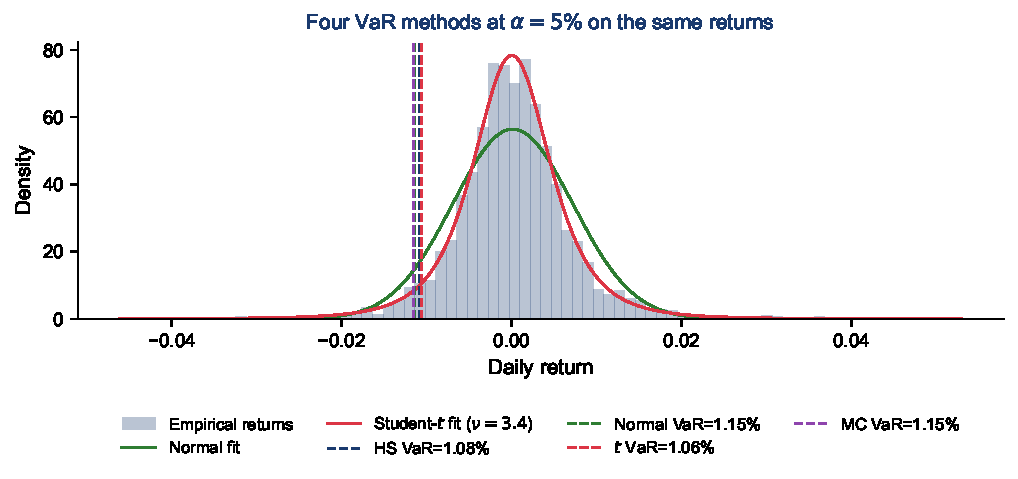
\includegraphics[width=\linewidth]{ch11_methods_comparison.pdf}
\figql{SFM\_ch11\_methods\_comparison}{https://github.com/danpele/SFM/tree/main/Quantlets/Ch_11/SFM_ch11_methods_comparison}
\end{column}
\end{columns}
\end{cminipage}
\end{frame}

%-----------------------------------------------------------------------------
% Filtered HS, Weighted HS, Cornish-Fisher
%-----------------------------------------------------------------------------

\slidelevel{MSc}
\begin{frame}{Filtered Historical Simulation (Hull--White 1998)}
\begin{cminipage}{0.96\textwidth}
\begin{columns}[T]
\begin{column}{0.50\textwidth}
\begin{block}{Idee: HS pe inova\c tii standardizate}
\begin{itemize}\setlength{\itemsep}{0pt}
    \item Filtreaz\u a randamentele cu un model GARCH: $z_t = (r_t - \mu_t)/\sigma_t$
    \item Aplic\u a HS pe $\{z_t\}$ (nu pe $r_t$)
    \item Scaleaz\u a cu volatilitatea curent\u a:
    \[
        \widehat{\VaR}_\alpha(t) = -\big(\mu_t + \sigma_t \cdot \hat{q}_\alpha(z)\big)
    \]
\end{itemize}
\end{block}
\begin{exampleblock}{Avantaje}
\begin{itemize}\setlength{\itemsep}{0pt}
    \item Combin\u a flexibilitatea HS cu reactivitatea GARCH
    \item Surprinde \textbf{cozile empirice} \c si \textbf{regimul curent}
    \item Folosit \^in industrie (Basel-approved)
\end{itemize}
\end{exampleblock}
\end{column}
\begin{column}{0.46\textwidth}
\centering
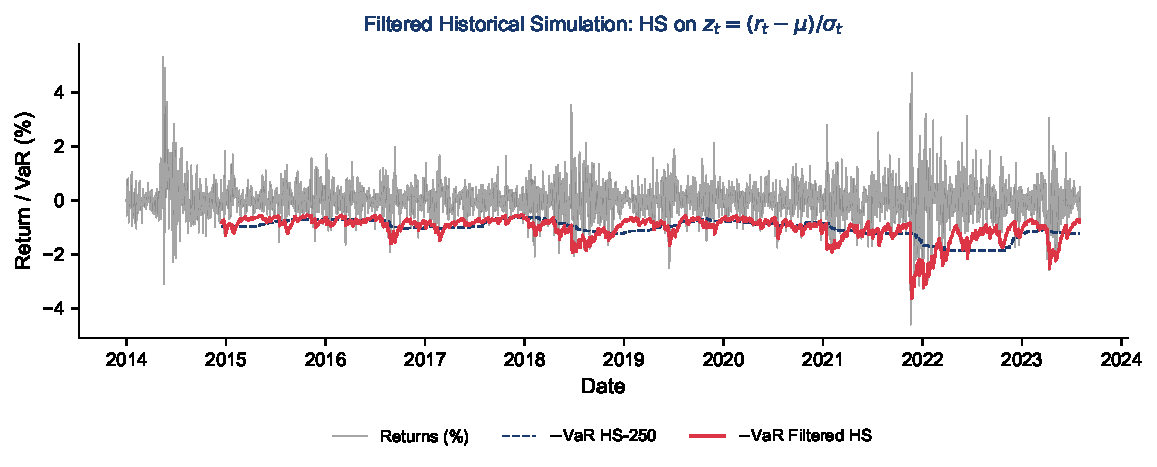
\includegraphics[width=\linewidth]{ch11_filtered_hs.pdf}\\[1pt]
{\scriptsize\textcolor{MediumGray}{\textit{FHS reac\c tioneaz\u a la \c socuri (Crimson) f\u ar\u a a pierde forma empiric\u a a cozii.}}}
\figql{SFM\_ch11\_filtered\_hs}{https://github.com/danpele/SFM/tree/main/Quantlets/Ch_11/SFM_ch11_filtered_hs}
\end{column}
\end{columns}
\end{cminipage}
\end{frame}

\slidelevel{MSc}
\begin{frame}[shrink=10]{Weighted Historical Simulation (Boudoukh et al.\ 1998)}
\begin{cminipage}{0.96\textwidth}
\begin{block}{Idee: ponderare exponen\c tial\u a a observa\c tiilor}
\begin{itemize}\setlength{\itemsep}{0pt}
    \item Atribuie observa\c tia $r_{t-i}$ ($i$ zile \^in trecut) o pondere:
    \[
        w_i = \lambda^i \cdot \frac{1-\lambda}{1-\lambda^W}, \quad \lambda \in (0,1)
    \]
    \item Cuantila empiric\u a ponderat\u a: sortare descresc\u atoare a pierderilor, $\widehat{\VaR}_\alpha$ = pierderea unde suma cumulativ\u a a ponderilor atinge $\alpha$
    \item RiskMetrics: $\lambda = 0{,}94$ (vol zilnic\u a) sau $\lambda = 0{,}97$ (lunar\u a)
\end{itemize}
\end{block}
\begin{columns}[T]
\begin{column}{0.50\textwidth}
\begin{exampleblock}{Avantaje vs HS standard}
\begin{itemize}\setlength{\itemsep}{0pt}
    \item Observa\c tiile recente conteaz\u a mai mult
    \item \textbf{Reduce ghost effect}: pierderea veche se ,,stinge'' exponen\c tial
    \item P\u astreaz\u a non-parametricitatea
\end{itemize}
\end{exampleblock}
\end{column}
\begin{column}{0.50\textwidth}
\begin{alertblock}{Limit\u ari}
\begin{itemize}\setlength{\itemsep}{0pt}
    \item Necesit\u a alegerea lui $\lambda$
    \item Effective sample size $\sim 1/(1-\lambda)$ poate fi mic
    \item La crize bru\c ste, \^inc\u a lag fa\c t\u a de GARCH
\end{itemize}
\end{alertblock}
\end{column}
\end{columns}
\end{cminipage}
\end{frame}

\slidelevel{MSc}
\begin{frame}[shrink=10]{Cornish-Fisher VaR (corec\c tie semi-parametric\u a)}
\begin{cminipage}{0.96\textwidth}
\begin{columns}[T]
\begin{column}{0.48\textwidth}
\begin{block}{Idee: ajustarea cuantilei Normal\u a}
\begin{itemize}\setlength{\itemsep}{0pt}
    \item Pornind de la $z_\alpha = \Phi^{-1}(\alpha)$:
    \begin{align*}
        z_\alpha^{CF} &= z_\alpha + \tfrac{(z_\alpha^2-1)S}{6}\\
        & + \tfrac{(z_\alpha^3-3z_\alpha)K}{24} - \tfrac{(2z_\alpha^3-5z_\alpha)S^2}{36}
    \end{align*}
    \item $S$ = skewness, $K$ = excess kurtosis
    \item $\VaR_\alpha^{CF} = -(\mu + \sigma z_\alpha^{CF})$
\end{itemize}
\end{block}
\begin{exampleblock}{C\^and folosi\c ti}
\begin{itemize}\setlength{\itemsep}{0pt}
    \item Cozi moderat de grele ($K < 8$)
    \item Avem nevoie de form\u a \^inchis\u a + corec\c tie pentru asimetrie
    \item NU pentru $\alpha < 1\%$ \^in cazuri foarte heavy
\end{itemize}
\end{exampleblock}
\end{column}
\begin{column}{0.50\textwidth}
\centering
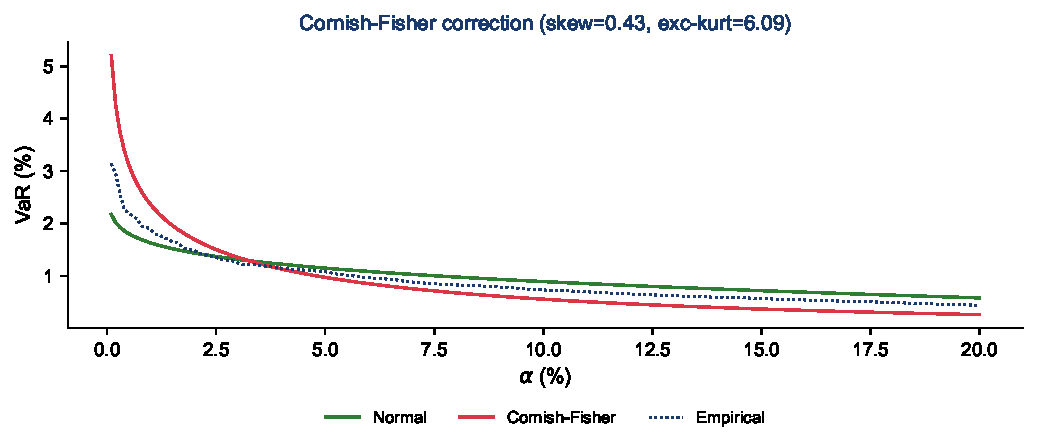
\includegraphics[width=\linewidth]{ch11_cornish_fisher.pdf}
\figql{SFM\_ch11\_cornish\_fisher}{https://github.com/danpele/SFM/tree/main/Quantlets/Ch_11/SFM_ch11_cornish_fisher}
\end{column}
\end{columns}
\end{cminipage}
\end{frame}

\slidelevel{MSc}
\begin{frame}[shrink=10]{Parametric skew-$t$: VaR pentru asimetrie}
\begin{cminipage}{0.96\textwidth}
\begin{itemize}\setlength{\itemsep}{1pt}
    \item Distribu\c tii Student-$t$ standard sunt simetrice; randamentele reale au \textbf{skewness negativ} (down-market crashes)
    \item \textbf{Hansen (1994) skew-$t$}: introduce parametru de asimetrie $\eta \in (-1, 1)$
    \[
        f(z;\,\nu,\eta) = \begin{cases} bc\Big(1+\tfrac{1}{\nu-2}\big(\tfrac{bz+a}{1-\eta}\big)^2\Big)^{-(\nu+1)/2} & z < -a/b \\
        bc\Big(1+\tfrac{1}{\nu-2}\big(\tfrac{bz+a}{1+\eta}\big)^2\Big)^{-(\nu+1)/2} & z \geq -a/b \end{cases}
    \]
    \item Constantele $a, b, c$ asigur\u a media 0 \c si varian\c ta 1
    \item Estimare: MLE pe randamentele standardizate
    \item Cuantila ajustat\u a $q_\alpha^{skew-t}$ se ob\c tine prin inversie numeric\u a
\end{itemize}
\vspace{0.1cm}
\begin{exampleblock}{C\^and folosi\c ti skew-$t$}
\begin{itemize}\setlength{\itemsep}{0pt}
    \item Randamente cu \textbf{asimetrie negativ\u a pronun\c tat\u a} (e.g., indici emergen\c ti)
    \item ETF-uri inverse / produse short-biased
    \item Modele GARCH cu inova\c tii skew-$t$ (\^ind GJR + skew-$t$)
\end{itemize}
\end{exampleblock}
\end{cminipage}
\end{frame}

\slidelevel{PhD}
\begin{frame}[shrink=10]{Quasi-Monte Carlo \c si importance sampling}
\begin{cminipage}{0.96\textwidth}
\begin{block}{Quasi-MC: secven\c te low-discrepancy}
\begin{itemize}\setlength{\itemsep}{0pt}
    \item \^Inlocuie\c ste numere pseudo-random cu secven\c te \textbf{Sobol} sau \textbf{Halton}
    \item Eroare: $O(1/M)$ \^in loc de $O(1/\sqrt{M})$ pentru integrale netede
    \item Util pentru cuantile moderate ($\alpha \in [1\%, 5\%]$)
\end{itemize}
\end{block}
\begin{block}{Importance Sampling (IS) pentru cuantile extreme}
\begin{itemize}\setlength{\itemsep}{0pt}
    \item Pentru $\alpha = 0{,}1\%$ sau mai mic: probabilitatea event \^in $M = 10^4$ e mic\u a
    \item IS: simuleaz\u a din $g(x)$ care concentreaz\u a probabilitate \^in coad\u a, apoi reponderez\u a:
    \[
        \widehat{p}_\alpha = \frac{1}{M}\sum_{i=1}^{M} \mathbb{1}\{X_i < -v\} \cdot \frac{f(X_i)}{g(X_i)}
    \]
    \item Cre\c stere de eficien\c t\u a: \textbf{$100\times$--$1000\times$} pentru cuantile $0{,}1\%$
    \item Referin\c ta: Glasserman, Heidelberger, Shahabuddin (2000)
\end{itemize}
\end{block}
\end{cminipage}
\end{frame}

%#############################################################################
\section{GARCH-VaR (condi\c tional)}
%#############################################################################

\slidelevel{MSc}
\begin{frame}{De ce VaR condi\c tional?}
\begin{cminipage}{0.95\textwidth}
\begin{itemize}\setlength{\itemsep}{1pt}
    \item \textbf{Volatility clustering} (stylized fact: cap. 6): perioade calme alterneaz\u a cu perioade volatile
    \item HS-VaR sau Normal-VaR \textbf{necondi\c tional} folosesc o singur\u a $\sigma$ pe \^intreaga fereastr\u a $\Rightarrow$ \textbf{r\u aspund lent} la \c socuri
    \item \textbf{Solu\c tia}: VaR condi\c tional de informa\c tia $\mathcal{F}_{t-1}$ disponibil\u a \^in $t-1$
    \[
        \VaR_\alpha(t) = -\big(\mu_t + \sigma_t \cdot q_\alpha(\varepsilon)\big),\quad
        \mu_t = \E[r_t \mid \mathcal{F}_{t-1}],\; \sigma_t^2 = \Var[r_t \mid \mathcal{F}_{t-1}]
    \]
    \item Pentru GARCH(1,1):
    \[
        \sigma_t^2 = \omega + \alpha\, (r_{t-1} - \mu)^2 + \beta\, \sigma_{t-1}^2
    \]
    \item Inova\c tiile $\varepsilon_t = (r_t - \mu_t)/\sigma_t$ se modeleaz\u a ca Normal, Student-$t$ sau GED
\end{itemize}
\end{cminipage}
\end{frame}

\slidelevel{MSc}
\begin{frame}{GARCH-VaR: implementare \c si exemplu}
\begin{cminipage}{0.96\textwidth}
\begin{columns}[T]
\begin{column}{0.48\textwidth}
\begin{block}{Etape de estimare}
\begin{enumerate}\setlength{\itemsep}{2pt}
    \item Fit GARCH(1,1)-$t$ pe seria $r_t$
    \item Extrage $\hat{\mu}$, $\hat{\sigma}_t$, $\hat{\nu}$ prin MLE
    \item Cuantila Student-$t$ standardizat\u a:
    \[ z_\alpha = t_{\hat{\nu}}^{-1}(\alpha) \sqrt{(\hat{\nu}-2)/\hat{\nu}} \]
    \item $\widehat{\VaR}_\alpha(t) = -(\hat{\mu}_t + \hat{\sigma}_t z_\alpha)$
\end{enumerate}
\end{block}
\vspace{0.15cm}
\begin{itemize}\setlength{\itemsep}{1pt}
    \item GARCH-VaR \textbf{r\u aspunde \^in 1--2 zile} la \c socuri
    \item HS-VaR \textbf{lag} c\^at fereastra ($W = 250$ zile)
\end{itemize}
\end{column}
\begin{column}{0.50\textwidth}
\centering
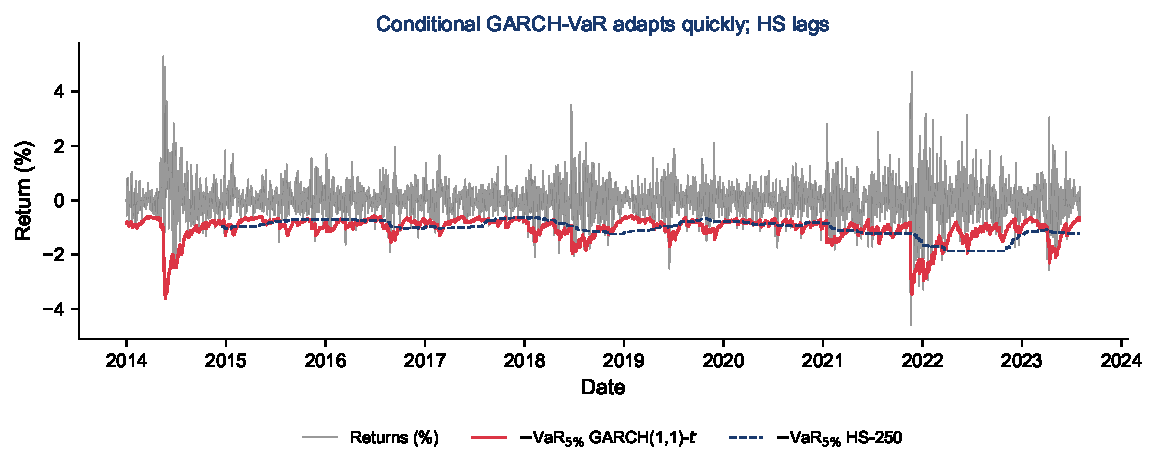
\includegraphics[width=\linewidth]{ch11_garch_var.pdf}\\[1pt]
{\scriptsize\textcolor{MediumGray}{\textit{GARCH(1,1)-$t$ vs.\ HS-250 pe acelea\c si date: GARCH se adapteaz\u a rapid; HS r\u am\^ane platou.}}}
\figql{SFM\_ch11\_garch\_var}{https://github.com/danpele/SFM/tree/main/Quantlets/Ch_11/SFM_ch11_garch_var}
\end{column}
\end{columns}
\end{cminipage}
\end{frame}

\slidelevel{MSc}
\begin{frame}{GJR-GARCH \c si EGARCH: leverage effect}
\begin{cminipage}{0.96\textwidth}
\begin{columns}[T]
\begin{column}{0.50\textwidth}
\begin{block}{GJR-GARCH (Glosten et al.\ 1993)}
\begin{itemize}\setlength{\itemsep}{0pt}
    \item Permite asimetrie: \c socurile negative cresc vol mai mult
    \[
        \sigma_t^2 = \omega + \alpha\varepsilon_{t-1}^2 + \gamma\varepsilon_{t-1}^2\mathbb{1}_{\varepsilon_{t-1}<0} + \beta\sigma_{t-1}^2
    \]
    \item $\gamma > 0$: \textbf{leverage effect} (verificat empiric)
\end{itemize}
\end{block}
\begin{block}{EGARCH (Nelson 1991)}
\begin{itemize}\setlength{\itemsep}{0pt}
    \item Logaritmic, garanteaz\u a $\sigma_t^2 > 0$:
    \[
        \ln\sigma_t^2 = \omega + \beta\ln\sigma_{t-1}^2 + \alpha\big(|z_{t-1}| - \E|z|\big) + \gamma z_{t-1}
    \]
    \item $\gamma < 0$ surprinde leverage
\end{itemize}
\end{block}
\end{column}
\begin{column}{0.46\textwidth}
\centering
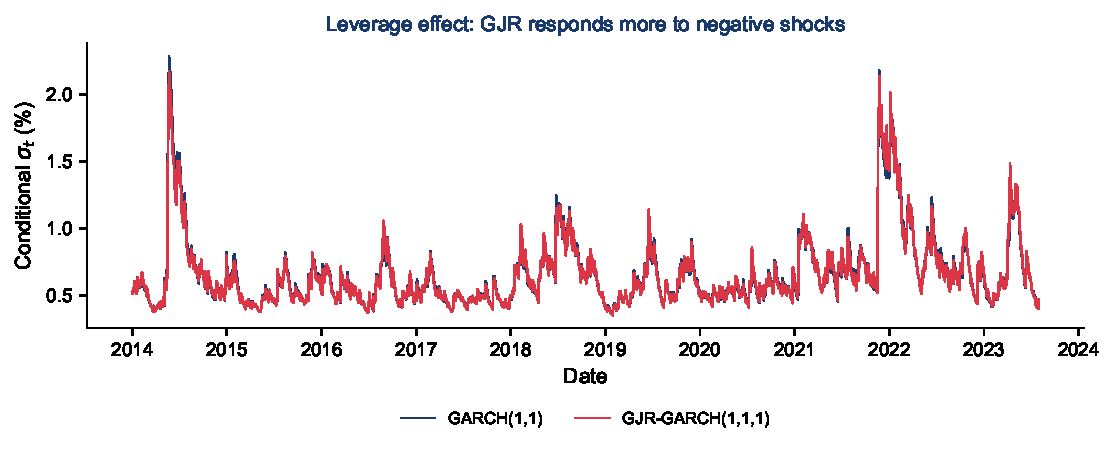
\includegraphics[width=\linewidth]{ch11_gjr_garch.pdf}\\[1pt]
{\scriptsize\textcolor{MediumGray}{\textit{GJR-GARCH (Crimson) urc\u a mai mult dup\u a \c socuri negative dec\^at GARCH simetric.}}}
\figql{SFM\_ch11\_gjr\_garch}{https://github.com/danpele/SFM/tree/main/Quantlets/Ch_11/SFM_ch11_gjr_garch}
\end{column}
\end{columns}
\end{cminipage}
\end{frame}

\slidelevel{PhD}
\begin{frame}[shrink=10]{Multivariate GARCH: DCC \c si BEKK pentru portofolii}
\begin{cminipage}{0.96\textwidth}
\begin{block}{DCC-GARCH (Engle 2002)}
\begin{itemize}\setlength{\itemsep}{0pt}
    \item Dou\u a etape: univariate GARCH per activ + corela\c tii dinamice
    \[
        H_t = D_t R_t D_t,\quad D_t = \operatorname{diag}(\sigma_{1,t}, \ldots, \sigma_{n,t}),\quad R_t = \text{Corr}_t(\varepsilon)
    \]
    \item $R_t = \operatorname{diag}(Q_t)^{-1/2} Q_t \operatorname{diag}(Q_t)^{-1/2}$, $Q_t$ matrice intermediar\u a
    \item Folosit pe portofolii: $\sigma_p^2(t) = \bm w^\top H_t \bm w$
\end{itemize}
\end{block}
\begin{block}{BEKK (Engle--Kroner 1995)}
\begin{itemize}\setlength{\itemsep}{0pt}
    \item Garanteaz\u a $H_t$ pozitiv definit\u a:
    \[
        H_t = CC^\top + A \varepsilon_{t-1}\varepsilon_{t-1}^\top A^\top + B H_{t-1} B^\top
    \]
    \item Costisitor pentru $n > 5$ active (parametri = $O(n^2)$)
    \item Solu\c tia produc\c tie: \textbf{DCC} (parsimon)
\end{itemize}
\end{block}
\end{cminipage}
\end{frame}

\slidelevel{PhD}
\begin{frame}[shrink=10]{Realized volatility \c si HAR-RV pentru VaR intraday}
\begin{cminipage}{0.96\textwidth}
\begin{block}{Realized Volatility (Andersen--Bollerslev 1998)}
\begin{itemize}\setlength{\itemsep}{0pt}
    \item Folose\c ste date intraday la $M$ frecven\c te:
    \[
        RV_t = \sum_{j=1}^{M} r_{t,j}^2 \xrightarrow{M\to\infty} \int_{t-1}^{t} \sigma^2(s)\, ds
    \]
    \item Estimator non-parametric, foarte precis pentru $\sigma_t$
\end{itemize}
\end{block}
\begin{block}{HAR-RV (Corsi 2009)}
\begin{itemize}\setlength{\itemsep}{0pt}
    \item Cascade de medii pe orizonturi diverse (zilnic, s\u apt\u am\^anal, lunar):
    \[
        \ln RV_t = \beta_0 + \beta_d \ln RV_{t-1} + \beta_w \ln RV_{t-1}^{(5)} + \beta_m \ln RV_{t-1}^{(22)} + u_t
    \]
    \item Capteaz\u a memorie lung\u a a volatilit\u a\c tii
    \item \textbf{VaR HAR-RV} bate GARCH la $\alpha = 1\%$ pe S\&P~500
\end{itemize}
\end{block}
\end{cminipage}
\end{frame}

%#############################################################################
\section{EVT: peaks-over-threshold (POT)}
%#############################################################################

\slidelevel{MSc}
\begin{frame}{Teorema Pickands--Balkema--de Haan}
\begin{cminipage}{0.95\textwidth}
\begin{thm}[Pickands 1975; Balkema--de Haan 1974]
\begin{itemize}\setlength{\itemsep}{0pt}
    \item Pentru o clas\u a larg\u a de distribu\c tii $F$, exist\u a $\beta(u) > 0$ astfel \^inc\^at, c\^and pragul $u \to x_F$ ($x_F = \sup\{x: F(x) < 1\}$):
    \[
        \Pr(L - u \leq y \mid L > u) \xrightarrow{u \to x_F} G_{\xi, \beta(u)}(y)
    \]
    \item $G_{\xi, \beta}$ este \textbf{Generalized Pareto Distribution} (GPD):
    \[
        G_{\xi,\beta}(y) = \begin{cases}
            1 - (1 + \xi y/\beta)^{-1/\xi} & \xi \neq 0 \\
            1 - \exp(-y/\beta) & \xi = 0
        \end{cases}, \quad y \geq 0
    \]
\end{itemize}
\end{thm}

\vspace{0.1cm}

\begin{itemize}\setlength{\itemsep}{1pt}
    \item $\xi$ -- \textbf{shape parameter}: $\xi > 0$ cozi grele (Pareto), $\xi = 0$ exponen\c tiale, $\xi < 0$ m\u arginite
    \item $\beta$ -- \textbf{scale parameter}: depinde de pragul $u$
    \item \textbf{Cheia EVT}: cozile au o form\u a \textit{universal\u a} (GPD), indiferent de centrul distribu\c tiei
\end{itemize}
\end{cminipage}
\end{frame}

\slidelevel{MSc}
\begin{frame}[shrink=10]{Estimarea VaR \c si ES via POT}
\begin{cminipage}{0.96\textwidth}
\begin{columns}[T]
\begin{column}{0.48\textwidth}
\begin{block}{Algoritm POT}
\begin{enumerate}\setlength{\itemsep}{0pt}
    \item Alege pragul $u$ (e.g., cuantila 90--95\% a pierderilor)
    \item Define\c ste exceden\c tele $Y_i = L_i - u$ pentru $L_i > u$
    \item Estimeaz\u a $(\hat\xi, \hat\beta)$ prin MLE pe GPD
    \item Calculeaz\u a:
    \[
        \VaR_\alpha = u + \frac{\hat\beta}{\hat\xi}\Big[\Big(\frac{n}{N_u}\alpha\Big)^{-\hat\xi} - 1\Big]
    \]
    \[
        \ES_\alpha = \frac{\VaR_\alpha}{1 - \hat\xi} + \frac{\hat\beta - \hat\xi u}{1-\hat\xi}
    \]
\end{enumerate}
\end{block}
\begin{itemize}\setlength{\itemsep}{0pt}
    \item $n$ -- num\u arul total de observa\c tii; $N_u$ -- num\u arul de exceden\c te
    \item ES finit doar dac\u a $\hat\xi < 1$
\end{itemize}
\end{column}
\begin{column}{0.50\textwidth}
\centering
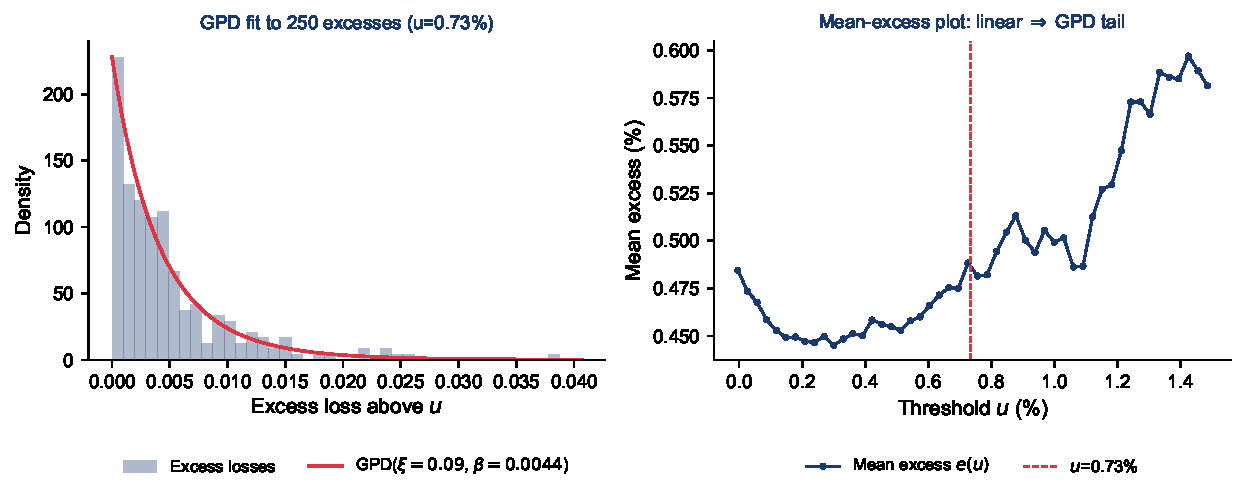
\includegraphics[width=\linewidth]{ch11_evt_var.pdf}\\[2pt]
{\scriptsize\textcolor{MediumGray}{\textit{St\^anga: GPD fit pe exceden\c te. Dreapta: mean-excess plot -- liniaritate $\Rightarrow$ GPD bun.}}}
\figql{SFM\_ch11\_evt\_var}{https://github.com/danpele/SFM/tree/main/Quantlets/Ch_11/SFM_ch11_evt_var}
\end{column}
\end{columns}
\end{cminipage}
\end{frame}

\slidelevel{MSc}
\begin{frame}[shrink=10]{Hill estimator pentru indexul de coad\u a}
\begin{cminipage}{0.96\textwidth}
\begin{columns}[T]
\begin{column}{0.50\textwidth}
\begin{block}{Hill (1975) -- estimator non-parametric pentru $\xi$}
\begin{itemize}\setlength{\itemsep}{0pt}
    \item Sorteaz\u a pierderile descresc\u ator: $L_{(1)} \geq L_{(2)} \geq \cdots \geq L_{(n)}$
    \item Pentru $k$ statistici extreme:
    \[
        \hat\xi_H(k) = \frac{1}{k} \sum_{i=1}^{k} \ln\frac{L_{(i)}}{L_{(k+1)}}
    \]
    \item Tail index Pareto: $\hat\alpha_H = 1/\hat\xi_H$
\end{itemize}
\end{block}
\begin{exampleblock}{Hill plot}
\begin{itemize}\setlength{\itemsep}{0pt}
    \item Reprezint\u a $\hat\alpha_H(k)$ ca func\c tie de $k$
    \item Alege $k^*$ \^in \textbf{regiunea stabil\u a} (platou)
    \item Compromis: bias (k mic) vs varian\c t\u a (k mare)
\end{itemize}
\end{exampleblock}
\end{column}
\begin{column}{0.46\textwidth}
\centering
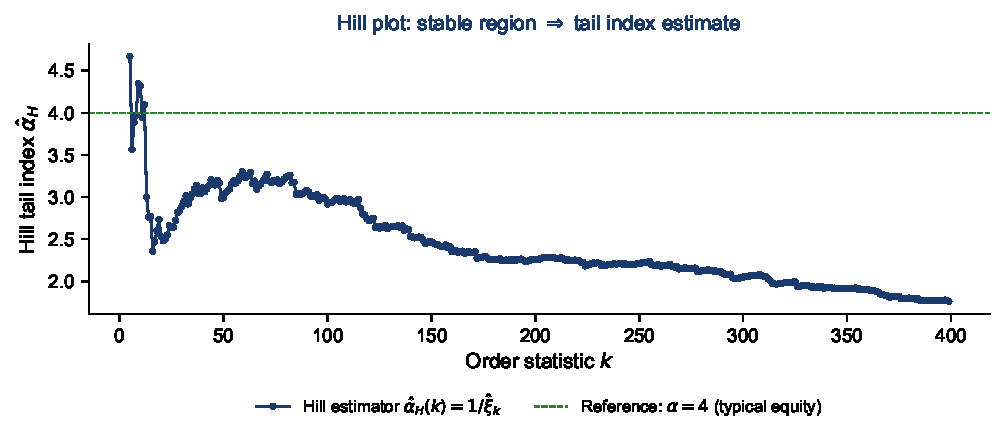
\includegraphics[width=\linewidth]{ch11_hill_plot.pdf}\\[1pt]
{\scriptsize\textcolor{MediumGray}{\textit{Hill plot: tail index estimate stabil \^in zona $k \in [50, 200]$.}}}
\figql{SFM\_ch11\_hill\_plot}{https://github.com/danpele/SFM/tree/main/Quantlets/Ch_11/SFM_ch11_hill_plot}
\end{column}
\end{columns}
\end{cminipage}
\end{frame}

\slidelevel{MSc}
\begin{frame}[shrink=15]{Block Maxima (BM) \c si GEV: o alternativ\u a la POT}
\begin{cminipage}{0.96\textwidth}
\begin{columns}[T]
\begin{column}{0.50\textwidth}
\begin{block}{Block Maxima -- Fisher--Tippett (1928)}
\begin{itemize}\setlength{\itemsep}{0pt}
    \item \^Imparte seria \^in blocuri ne-suprapuse (e.g., lunare, $b = 20$ zile)
    \item Re\c tine maximul fiec\u arui bloc: $M_j = \max\{L_{(j-1)b+1}, \ldots, L_{jb}\}$
    \item Distribu\c tia limit\u a: \textbf{Generalized Extreme Value (GEV)}
    \[
        H_{\xi}(x) = \exp\Big(-\big(1+\xi\tfrac{x-\mu}{\sigma}\big)^{-1/\xi}\Big)
    \]
\end{itemize}
\end{block}
\begin{exampleblock}{BM vs POT}
\begin{itemize}\setlength{\itemsep}{0pt}
    \item POT folose\c ste \textbf{mai mult\u a} informa\c tie (toate dep\u a\c sirile, nu doar maximul)
    \item BM mai potrivit\u a c\^and avem date trimestriale/anuale
    \item Echivalente asimptotic: $\xi^{GEV} = \xi^{GPD}$
\end{itemize}
\end{exampleblock}
\end{column}
\begin{column}{0.46\textwidth}
\centering
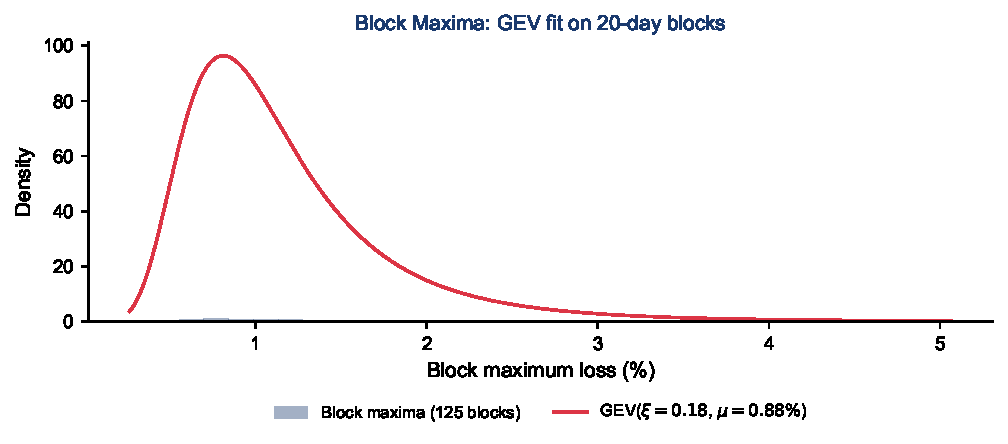
\includegraphics[width=\linewidth]{ch11_block_maxima.pdf}\\[1pt]
{\scriptsize\textcolor{MediumGray}{\textit{GEV fit pe maximele blocurilor 20-day din seria simulat\u a.}}}
\figql{SFM\_ch11\_block\_maxima}{https://github.com/danpele/SFM/tree/main/Quantlets/Ch_11/SFM_ch11_block_maxima}
\end{column}
\end{columns}
\end{cminipage}
\end{frame}

\slidelevel{MSc}
\begin{frame}[shrink=15]{Formula explicit\u a EVT-ES (sub GPD)}
\begin{cminipage}{0.96\textwidth}
\begin{block}{ES sub Generalized Pareto}
\begin{itemize}\setlength{\itemsep}{0pt}
    \item Condi\c tie de existen\c t\u a: $\xi < 1$ (altfel ES infinit)
    \item Formula explicit\u a:
    \[
        \widehat{\ES}_\alpha = \frac{\widehat{\VaR}_\alpha}{1-\hat\xi} + \frac{\hat\beta - \hat\xi u}{1-\hat\xi}
    \]
    \item $u$ -- pragul POT
    \item $\hat\beta$ -- scale parameter GPD
    \item $\hat\xi$ -- shape parameter (tail index)
\end{itemize}
\end{block}
\begin{exampleblock}{Exemplu numeric}
\begin{itemize}\setlength{\itemsep}{0pt}
    \item Date: $u = 2{,}0\%$, $\hat\xi = 0{,}15$, $\hat\beta = 0{,}8\%$
    \item $\widehat{\VaR}_{1\%} = u + (\hat\beta/\hat\xi)\big((n/N_u\cdot\alpha)^{-\hat\xi}-1\big) \approx 3{,}5\%$
    \item $\widehat{\ES}_{1\%} = 3{,}5\%/(1-0{,}15) + (0{,}8\%-0{,}15\cdot 2{,}0\%)/(1-0{,}15) \approx 4{,}71\%$
    \item Ratio ES/VaR = $4{,}71\%/3{,}5\% \approx 1{,}35$ (tipic pentru cozi grele)
\end{itemize}
\end{exampleblock}
\end{cminipage}
\end{frame}

%#############################################################################
\section{Expected Shortfall (ES)}
%#############################################################################

\slidelevel{Y3}
\begin{frame}{Limita esen\c tial\u a a VaR: ce se \^int\^ampl\u a \textit{dincolo}?}
\begin{cminipage}{0.95\textwidth}
\begin{itemize}\setlength{\itemsep}{1pt}
    \item VaR spune doar \textbf{pragul} pierderii: $\VaR_{1\%} = 35.000$~EUR
    \item Dar \textbf{c\^at de mare e pierderea}, dat fiind c\u a am dep\u a\c sit pragul?
    \item Dou\u a portofolii cu acela\c si $\VaR_{1\%}$ pot avea pierderi medii \^in coad\u a \textit{foarte diferite}:
\end{itemize}
\vspace{0.1cm}
\begin{center}
\renewcommand{\arraystretch}{1.15}
\small
\begin{tabular}{lcc}
\toprule
& \textbf{Portofoliu A} & \textbf{Portofoliu B} \\
\midrule
$\VaR_{1\%}$  & 35.000 EUR & 35.000 EUR \\
Pierdere medie \^in cele mai rele 1\% zile & 38.000 EUR & 120.000 EUR \\
$\ES_{1\%}$   & 38.000 EUR & 120.000 EUR \\
\bottomrule
\end{tabular}
\end{center}
\vspace{0.15cm}
\begin{alertblock}{Concluzia}
\begin{itemize}\setlength{\itemsep}{0pt}
    \item VaR \textbf{nu poate distinge} cele dou\u a portofolii (ambele au $\VaR_{1\%} = 35.000$ EUR)
    \item ES \textbf{distinge}: 38.000 EUR vs 120.000 EUR
\end{itemize}
\end{alertblock}
\end{cminipage}
\end{frame}

\slidelevel{MSc}
\begin{frame}[shrink=25]{Defini\c tia formal\u a a Expected Shortfall}
\begin{cminipage}{0.96\textwidth}
\begin{defn}[Expected Shortfall, CVaR, Tail-VaR]
\begin{itemize}\setlength{\itemsep}{0pt}
    \item Condi\c tii: distribu\c tii continue, $\alpha \in (0,1)$
    \item Pe pierderea $L$:
    \[
        \ES_\alpha(L) = \frac{1}{\alpha}\int_0^\alpha \VaR_u(L)\, du = \E[L \mid L \geq \VaR_\alpha(L)]
    \]
    \item Echivalent pe rentabilitatea $X = -L$:
    \[
        \ES_\alpha(X) = -\frac{1}{\alpha}\int_0^\alpha F_X^{-1}(p)\, dp = -\E[X \mid X \leq -\VaR_\alpha]
    \]
\end{itemize}
\end{defn}

\vspace{0.1cm}

\begin{block}{Interpretare}
\begin{itemize}\setlength{\itemsep}{0pt}
    \item ES = media pierderilor \^in cele mai rele $\alpha\%$ zile
    \item Surprinde explicit severitatea cozii (nu doar pragul)
\end{itemize}
\end{block}

\begin{exampleblock}{Formule \^inchise}
\begin{itemize}\setlength{\itemsep}{0pt}
    \item Sub Normal\u a: $\ES_\alpha = -\mu + \sigma \cdot \phi(z_\alpha)/\alpha$
    \item Sub Student-$t$ standardizat ($\nu > 1$): vezi cap. 5
\end{itemize}
\end{exampleblock}
\end{cminipage}
\end{frame}

\slidelevel{MSc}
\begin{frame}{VaR vs ES --- vizualizare \c si nota\c tii}
\begin{cminipage}{0.96\textwidth}
\begin{columns}[T]
\begin{column}{0.50\textwidth}
\begin{itemize}\setlength{\itemsep}{1pt}
    \item \textbf{VaR}: prag (frontiera ro\c sie a cozii)
    \item \textbf{ES}: media \textit{tuturor} valorilor din coada ro\c sie
    \item \^In general $\ES_\alpha \geq \VaR_\alpha$ (egalitate doar pentru distribu\c tii degenerate)
    \item Sub Normal $\alpha = 5\%$:
    \[
        \VaR_{5\%} = 1{,}64\sigma, \quad \ES_{5\%} = 2{,}06\sigma
    \]
    \item Sub Normal $\alpha = 1\%$:
    \[
        \VaR_{1\%} = 2{,}33\sigma, \quad \ES_{1\%} = 2{,}67\sigma
    \]
    \item \textbf{FRTB}: ES 97{,}5\% al pierderilor $\approx$ VaR 99\% al pierderilor (\^in sens regulator)
\end{itemize}
\end{column}
\begin{column}{0.46\textwidth}
\centering
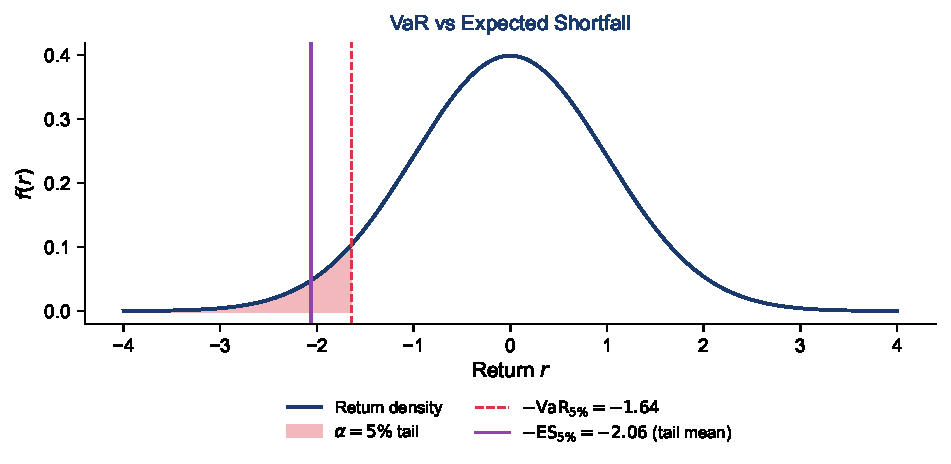
\includegraphics[width=\linewidth]{ch11_var_es_concept.pdf}
\figql{SFM\_ch11\_var\_concept}{https://github.com/danpele/SFM/tree/main/Quantlets/Ch_11/SFM_ch11_var_concept}
\end{column}
\end{columns}
\end{cminipage}
\end{frame}

\slidelevel{MSc}
\begin{frame}[shrink=10]{Raportul ES/VaR: c\^at de important sunt cozile?}
\begin{cminipage}{0.96\textwidth}
\begin{columns}[T]
\begin{column}{0.42\textwidth}
\begin{block}{Insight cheie}
\begin{itemize}\setlength{\itemsep}{0pt}
    \item ES/VaR cre\c ste c\^and:
    \begin{itemize}\setlength{\itemsep}{0pt}
        \item $\alpha$ scade (cuantile mai extreme)
        \item Cozile sunt mai grele ($\nu$ mai mic la Student-$t$)
    \end{itemize}
    \item Sub Normal\u a, $\alpha=5\%$: ES/VaR $\approx 1{,}25$
    \item Sub Student-$t_3$, $\alpha=0{,}1\%$: ES/VaR $\approx 2{,}0$ sau mai mult!
\end{itemize}
\end{block}
\begin{exampleblock}{Implica\c tii practice}
\begin{itemize}\setlength{\itemsep}{0pt}
    \item Sub FRTB: ES 97,5\% \^inlocuie\c ste VaR 99\% (Normal\u a $\Rightarrow$ aproximativ acela\c si)
    \item Sub cozi grele: ES 97,5\% \textbf{depa\c se\c ste} VaR 99\%
    \item Capital regulatory mai mare pentru active cu cozi grele
\end{itemize}
\end{exampleblock}
\end{column}
\begin{column}{0.56\textwidth}
\centering
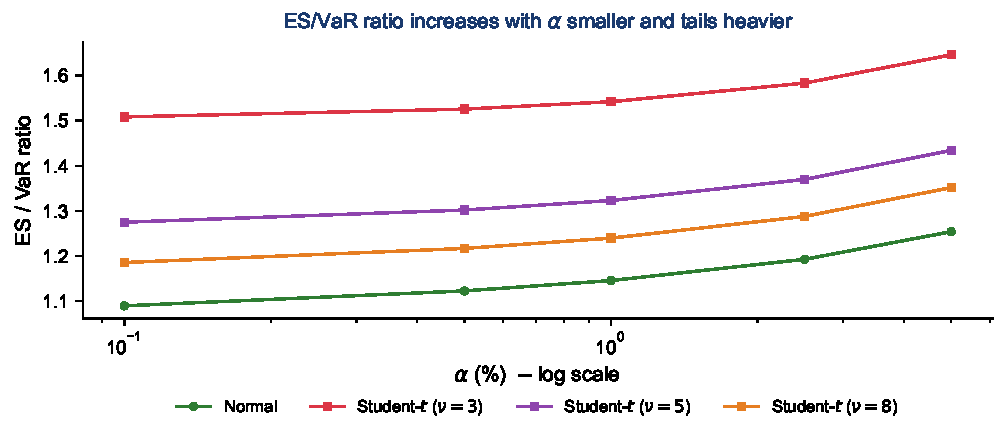
\includegraphics[width=\linewidth]{ch11_es_var_ratio.pdf}\\[1pt]
{\scriptsize\textcolor{MediumGray}{\textit{Raportul ES/VaR diverge c\^and $\alpha \to 0$ \c si coada devine mai grea.}}}
\figql{SFM\_ch11\_es\_var\_ratio}{https://github.com/danpele/SFM/tree/main/Quantlets/Ch_11/SFM_ch11_es_var_ratio}
\end{column}
\end{columns}
\end{cminipage}
\end{frame}

\slidelevel{PhD}
\begin{frame}{ES decomposition: contribu\c tia per activ (Euler allocation)}
\begin{cminipage}{0.96\textwidth}
\begin{block}{Decompozi\c tia Euler pentru ES}
\begin{itemize}\setlength{\itemsep}{0pt}
    \item Fie $L = \sum_i w_i L_i$ pierderea total\u a a portofoliului
    \item Sub omogenitate (axioma A3): $\ES_\alpha(L) = \sum_i w_i \cdot \text{ES}_\alpha^i$
    \item Contribu\c tia per activ:
    \[
        \text{ES}_\alpha^i = \E[L_i \mid L \geq \VaR_\alpha(L)]
    \]
\end{itemize}
\end{block}
\begin{exampleblock}{Aplica\c tii}
\begin{itemize}\setlength{\itemsep}{0pt}
    \item \textbf{Risk budgeting}: aloc\u a capital propor\c tional cu contribu\c tia ES
    \item \textbf{Hedge ratios}: prioritizeaz\u a hedging activele cu cea mai mare $\text{ES}_\alpha^i$
    \item \textbf{Performance measurement}: $\text{RAROC}_i = \E[r_i]/\text{ES}_\alpha^i$
    \item \textbf{Aproximare}: dificil de estimat din date pu\c tine; folose\c ste MC sau IS
\end{itemize}
\end{exampleblock}
\end{cminipage}
\end{frame}

%#############################################################################
\section{M\u asuri coerente de risc}
%#############################################################################

\slidelevel{MSc}
\begin{frame}[shrink=15]{Axiomele Artzner et al.\ (1999)}
\begin{cminipage}{0.95\textwidth}
\begin{defn}[M\u asur\u a coerent\u a de risc]
\begin{itemize}\setlength{\itemsep}{0pt}
    \item O func\c tional\u a $\rho: \mathcal{X} \to \R$ este \textbf{coerent\u a} dac\u a satisface axiomele A1--A4 de mai jos
\end{itemize}
\end{defn}
\begin{enumerate}\setlength{\itemsep}{2pt}
    \item[\textcolor{MainBlue}{\textbf{A1.}}] \textbf{Monotonie}: $X \leq Y \Rightarrow \rho(X) \geq \rho(Y)$
    \begin{itemize}\setlength{\itemsep}{0pt}
        \item Pierderi mai mari $\Rightarrow$ risc mai mare
    \end{itemize}
    \item[\textcolor{MainBlue}{\textbf{A2.}}] \textbf{Subaditivitate}: $\rho(X+Y) \leq \rho(X) + \rho(Y)$
    \begin{itemize}\setlength{\itemsep}{0pt}
        \item Diversificarea nu cre\c ste riscul
    \end{itemize}
    \item[\textcolor{MainBlue}{\textbf{A3.}}] \textbf{Omogenitate pozitiv\u a}: $\rho(\lambda X) = \lambda \rho(X)$ pentru $\lambda > 0$
    \begin{itemize}\setlength{\itemsep}{0pt}
        \item Dublarea pozi\c tiei dubleaz\u a riscul (scale invariance)
    \end{itemize}
    \item[\textcolor{MainBlue}{\textbf{A4.}}] \textbf{Invarian\c t\u a la transla\c tie}: $\rho(X + c) = \rho(X) - c$ pentru $c \in \R$
    \begin{itemize}\setlength{\itemsep}{0pt}
        \item Ad\u augarea de numerar reduce riscul cu aceea\c si sum\u a (cash-additive)
    \end{itemize}
\end{enumerate}
\vspace{0.2cm}
\begin{alertblock}{Rezultat cheie (Acerbi--Tasche 2002)}
\begin{itemize}\setlength{\itemsep}{0pt}
    \item \textbf{ES satisface toate cele 4 axiome} $\Rightarrow$ ES este coerent\u a
    \item \textbf{VaR e\c sueaz\u a A2} (subaditivitatea) \^in general; este coerent\u a doar sub distribu\c tii eliptice (e.g., Normal\u a)
\end{itemize}
\end{alertblock}
\end{cminipage}
\end{frame}

\slidelevel{PhD}
\begin{frame}[shrink=10]{Spectrale: o familie mai larg\u a de m\u asuri coerente}
\begin{cminipage}{0.95\textwidth}
\begin{defn}[M\u asur\u a spectral\u a de risc, Acerbi 2002]
\begin{itemize}\setlength{\itemsep}{0pt}
    \item Formul\u a: $\rho_\phi(X) = -\int_0^1 F_X^{-1}(p) \cdot \phi(p)\, dp$
    \item $\phi: [0,1] \to \R_+$ este func\c tie de aversiune fa\c t\u a de risc nedescresc\u atoare
    \item Normalizare: $\int_0^1 \phi(p)\, dp = 1$
\end{itemize}
\end{defn}
\vspace{0.15cm}
\begin{itemize}\setlength{\itemsep}{1pt}
    \item \textbf{Cazuri particulare}:
    \begin{itemize}\setlength{\itemsep}{0pt}
        \item $\phi(p) = \mathbb{1}_{p \leq \alpha} / \alpha$ $\Rightarrow$ ES la nivel $\alpha$
        \item $\phi(p) = \delta_\alpha$ $\Rightarrow$ VaR (\textbf{nu este} nedescresc\u atoare $\Rightarrow$ NU este spectral\u a)
    \end{itemize}
    \item \textbf{M\u asurile spectrale} sunt coerente \c si \textbf{lipsite de cozi ascunse}
    \item Genereaz\u a m\u asuri precum \textbf{distortion} (Wang 2000) \c si \textbf{Choquet expected utility}
\end{itemize}
\vspace{0.15cm}
\begin{block}{De ce conteaz\u a pentru regulator?}
\begin{itemize}\setlength{\itemsep}{0pt}
    \item M\u asurile spectrale pot fi calibrate la \textit{aversiunea fa\c t\u a de risc} a regulatorului
    \item FRTB folose\c ste implicit o ES cu $\alpha = 2{,}5\%$
\end{itemize}
\end{block}
\end{cminipage}
\end{frame}

%#############################################################################
\section{Estimare rolling}
%#############################################################################

\slidelevel{Y3}
\begin{frame}{Rolling VaR \c si ES: metodologie}
\begin{cminipage}{0.95\textwidth}
\begin{block}{Algoritm rolling window}
\begin{itemize}\setlength{\itemsep}{0pt}
    \item Date: seria $\{r_1, \ldots, r_T\}$ \c si dimensiunea ferestrei $W$ (e.g., $W = 250$)
    \item Pentru fiecare $t = W+1, \ldots, T$:
    \begin{itemize}\setlength{\itemsep}{0pt}
        \item Selecteaz\u a fereastra $\{r_{t-W}, \ldots, r_{t-1}\}$
        \item Estimeaz\u a $\widehat{\VaR}_\alpha(t)$ \c si $\widehat{\ES}_\alpha(t)$ pe acea fereastr\u a
    \end{itemize}
    \item Calculeaz\u a \textbf{excep\c tia} (hit): $I_t = \mathbb{1}\{r_t < -\widehat{\VaR}_\alpha(t)\}$
    \item Raporteaz\u a $\{(\widehat{\VaR}_\alpha(t), I_t)\}_{t=W+1}^{T}$ pentru backtesting
\end{itemize}
\end{block}

\vspace{0.15cm}
\begin{block}{Alegerea ferestrei $W$}
\begin{itemize}\setlength{\itemsep}{0pt}
    \item $W = 250$ zile: standard Basel; suficient pentru $\alpha = 1\%$ ($\sim 2{,}5$ exceden\c te a\c steptate)
    \item $W = 500$: rezolu\c tie mai bun\u a la cuantile extreme, dar adaptare mai lent\u a
    \item $W < 100$: instabilitate; recomandat doar pentru GARCH (unde estim\u am parametri, nu cuantile)
\end{itemize}
\end{block}
\end{cminipage}
\end{frame}

\slidelevel{Y3}
\begin{frame}{Rolling VaR/ES --- exemplu pe randamente simulate}
\begin{cminipage}{0.96\textwidth}
\begin{columns}[T]
\begin{column}{0.55\textwidth}
\begin{itemize}\setlength{\itemsep}{1pt}
    \item Date: 2500 randamente zilnice GARCH-$t$
    \item Trei estim\u ari rolling cu $W = 250$, $\alpha = 5\%$:
    \begin{itemize}\setlength{\itemsep}{0pt}
        \item $\widehat{\VaR}^{HS}$ (Historical Simulation)
        \item $\widehat{\VaR}^{N}$ (Parametric\u a Normal\u a)
        \item $\widehat{\ES}^{HS}$ (Historical Simulation)
    \end{itemize}
    \item Punctele ro\c sii: zile \^in care $r_t < -\widehat{\VaR}_t$ (excep\c tii)
    \item \textbf{Observa\c tii}:
    \begin{itemize}\setlength{\itemsep}{0pt}
        \item Viol\u arile apar \textit{clusterizat} \^in jurul cre\c sterilor de volatilitate
        \item HS \c si Normal\u a converg \^in regim calm, diverg \^in regim volatil
    \end{itemize}
\end{itemize}
\end{column}
\begin{column}{0.42\textwidth}
\centering
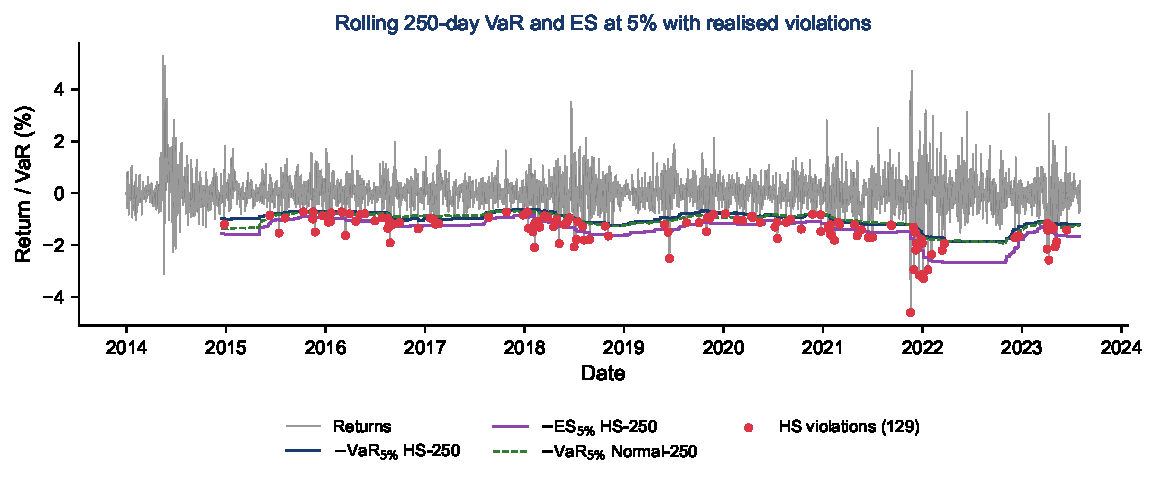
\includegraphics[width=\linewidth]{ch11_rolling_var_es.pdf}
\figql{SFM\_ch11\_rolling\_var\_es}{https://github.com/danpele/SFM/tree/main/Quantlets/Ch_11/SFM_ch11_rolling_var_es}
\end{column}
\end{columns}
\end{cminipage}
\end{frame}

\slidelevel{MSc}
\begin{frame}[shrink=10]{Implementare rolling: schi\c t\u a algoritmic\u a}
\begin{cminipage}{0.95\textwidth}
\begin{block}{Pseudocod}
\begin{enumerate}\setlength{\itemsep}{1pt}
    \item Pentru fiecare $t = W+1, \ldots, T$:
    \begin{itemize}\setlength{\itemsep}{0pt}
        \item Selecteaz\u a fereastra $w_t = \{r_{t-W}, \ldots, r_{t-1}\}$
        \item Cuantila empiric\u a $q_t = Q_\alpha(w_t)$
        \item $\widehat{\VaR}_\alpha(t) = -q_t$, $\widehat{\ES}_\alpha(t) = -\overline{w_t \mid w_t \le q_t}$
    \end{itemize}
    \item Construie\c ste hit-sequence $I_t = \mathbb{1}\{r_t < -\widehat{\VaR}_\alpha(t)\}$
    \item Verific\u a rata observat\u a $\bar{I} \approx \alpha$
\end{enumerate}
\end{block}
\vspace{0.15cm}
\begin{block}{Recomand\u ari pentru produc\c tie}
\begin{itemize}\setlength{\itemsep}{0pt}
    \item Folosi\c ti \texttt{pandas.Series.rolling(window).quantile(alpha)} pentru vitez\u a
    \item Pentru EVT-rolling: refit GPD doar la fiecare $k$ zile (reducere cost)
    \item Pentru GARCH-rolling: refit la 5--20 zile, prognoz\u a 1-day ahead
\end{itemize}
\end{block}
\vspace{0.1cm}
\begin{center}
\quantlet{SFM\_ch11\_rolling\_var\_es}{https://github.com/danpele/SFM/tree/main/Quantlets/Ch_11/SFM_ch11_rolling_var_es}
\end{center}
\end{cminipage}
\end{frame}

%#############################################################################
\section{Backtesting VaR}
%#############################################################################

\slidelevel{Y3}
\begin{frame}{Ce \^inseamn\u a un backtest VaR?}
\begin{cminipage}{0.95\textwidth}
\begin{itemize}\setlength{\itemsep}{1pt}
    \item Pentru fiecare zi $t$: comparam $r_t$ cu $-\widehat{\VaR}_\alpha(t)$ prognozat \^in $t-1$
    \item Define\c ste \textbf{hit sequence} (Christoffersen 1998):
    \[
        I_t = \mathbb{1}\{r_t < -\widehat{\VaR}_\alpha(t)\}, \quad t = 1, \ldots, T
    \]
    \item Sub modelul \textbf{corect}, $\{I_t\}$ ar trebui s\u a fie:
    \begin{itemize}\setlength{\itemsep}{0pt}
        \item \textbf{(P1) Acoperire necondi\c tional\u a}: $\E[I_t] = \alpha$ (frecven\c ta corect\u a)
        \item \textbf{(P2) Independen\c t\u a}: $I_t \perp I_{t-k}$ (f\u ar\u a clustering)
        \item \textbf{(P3) Acoperire condi\c tional\u a}: $\Pr(I_t = 1 \mid \mathcal{F}_{t-1}) = \alpha$ ((P1)+(P2))
    \end{itemize}
    \item \textbf{Trei teste clasice}:
    \begin{itemize}\setlength{\itemsep}{0pt}
        \item \textbf{Kupiec POF} -- testeaz\u a (P1)
        \item \textbf{Christoffersen IC} -- testeaz\u a (P2)
        \item \textbf{Christoffersen CC} -- testeaz\u a (P3) (= POF + IC)
    \end{itemize}
\end{itemize}
\end{cminipage}
\end{frame}

\slidelevel{MSc}
\begin{frame}[shrink=10]{Testul Kupiec (1995) -- Proportion of Failures}
\begin{cminipage}{0.95\textwidth}
\begin{block}{Construc\c tia testului}
\begin{itemize}\setlength{\itemsep}{0pt}
    \item Ipoteze: $H_0$: $\Pr(I_t = 1) = \alpha$ \quad vs.\ \quad $H_1$: $\Pr(I_t = 1) \neq \alpha$
    \item Notatii: $x = \sum_{t=1}^n I_t$ \c si $\hat p = x/n$
    \item Statistica testului:
    \[
        LR_{POF} = -2 \ln\frac{\alpha^x (1-\alpha)^{n-x}}{\hat p^{\, x} (1-\hat p)^{n-x}} \xrightarrow{H_0} \chi^2_1
    \]
    \item Decizie: respingem $H_0$ dac\u a $LR_{POF} > \chi^2_1(0{,}95) = 3{,}84$
\end{itemize}
\end{block}

\begin{columns}[T]
\begin{column}{0.50\textwidth}
\textbf{Exemplu numeric ($n = 250$, $\alpha = 5\%$)}
\begin{itemize}\setlength{\itemsep}{0pt}
    \item Excep\c tii a\c steptate: $n\alpha = 12{,}5$
    \item Excep\c tii observate: $x = 18$
    \item $\hat p = 18/250 = 0{,}072$
    \item $LR_{POF} = 2{,}43$, $p$-value $= 0{,}119$
    \item \textbf{Concluzie}: nu respingem $H_0$ la 5\%
\end{itemize}
\end{column}
\begin{column}{0.48\textwidth}
\centering
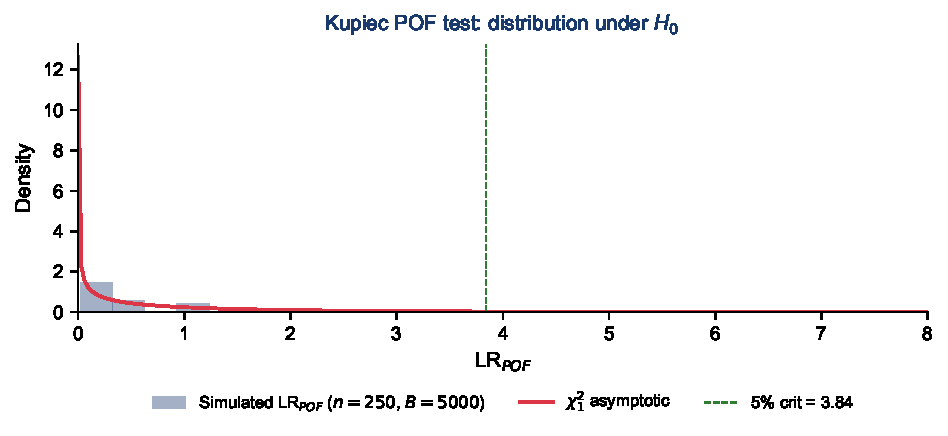
\includegraphics[width=\linewidth]{ch11_kupiec_distribution.pdf}
\figql{SFM\_ch11\_kupiec}{https://github.com/danpele/SFM/tree/main/Quantlets/Ch_11/SFM_ch11_kupiec}
\end{column}
\end{columns}
\end{cminipage}
\end{frame}

\slidelevel{MSc}
\begin{frame}[shrink=5]{Testul Christoffersen (1998) -- Independence}
\begin{cminipage}{0.95\textwidth}
\begin{block}{Idee: lan\c t Markov de ordin 1 pe $\{I_t\}$}
\begin{itemize}\setlength{\itemsep}{0pt}
    \item Contoriz\u am tranzi\c tiile: $n_{ij} = \#\{t : I_{t-1}=i,\, I_t=j\}$
    \item Probabilit\u a\c tile de tranzi\c tie: $\pi_{ij} = n_{ij} / (n_{i0} + n_{i1})$
    \item $H_0$ (independen\c t\u a): $\pi_{01} = \pi_{11} = \pi_2$, unde $\pi_2 = (n_{01}+n_{11})/n$
    \item Statistica testului IC:
    \[
        LR_{IC} = -2 \ln\frac{(1-\pi_2)^{n_{00}+n_{10}} \pi_2^{n_{01}+n_{11}}}{(1-\pi_{01})^{n_{00}} \pi_{01}^{n_{01}} (1-\pi_{11})^{n_{10}} \pi_{11}^{n_{11}}} \xrightarrow{H_0} \chi^2_1
    \]
\end{itemize}
\end{block}
\begin{itemize}\setlength{\itemsep}{1pt}
    \item Testul \textbf{Conditional Coverage} (CC):
    \[
        LR_{CC} = LR_{POF} + LR_{IC} \xrightarrow{H_0} \chi^2_2
    \]
    \item \textbf{De ce conteaz\u a?} Un model care produce excep\c tii \textit{clusterizate} \^inseamn\u a c\u a NU surprinde regimul de volatilitate
\end{itemize}
\end{cminipage}
\end{frame}

\slidelevel{MSc}
\begin{frame}{Viol\u ari: independente vs.\ clusterizate}
\begin{cminipage}{0.96\textwidth}
\begin{columns}[T]
\begin{column}{0.42\textwidth}
\begin{itemize}\setlength{\itemsep}{1pt}
    \item \textbf{Sus}: excep\c tii Bernoulli iid (model bun)
    \item \textbf{Jos}: excep\c tii Markov clusterizate (model prost), $\pi_{01} = 2\%$, $\pi_{11} = 40\%$
    \item Ambele au $\sim 13$ excep\c tii pe 250 zile $\Rightarrow$ \textbf{Kupiec nu poate distinge}
    \item Christoffersen IC \textbf{respinge} cazul de jos
    \item \textbf{Concluzie}: testele Kupiec \c si Christoffersen sunt complementare; raporta\c ti \textbf{ambele}
\end{itemize}
\end{column}
\begin{column}{0.56\textwidth}
\centering
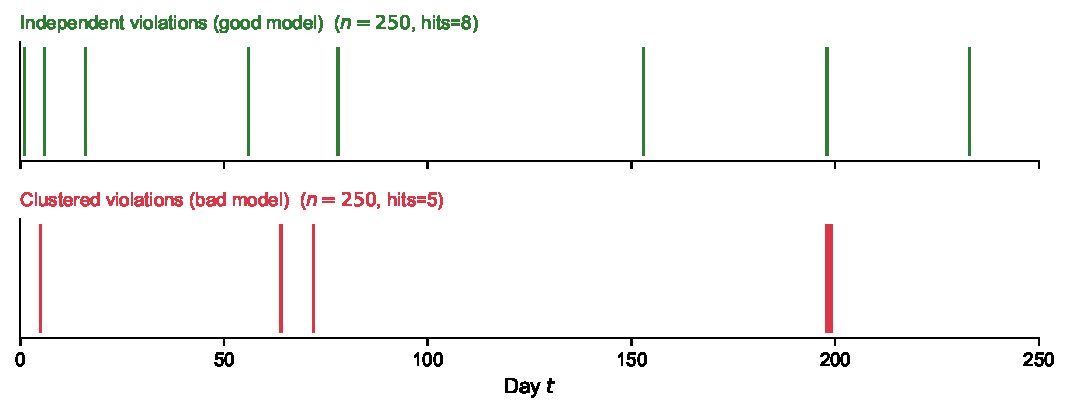
\includegraphics[width=\linewidth]{ch11_christoffersen_clustering.pdf}
\figql{SFM\_ch11\_christoffersen}{https://github.com/danpele/SFM/tree/main/Quantlets/Ch_11/SFM_ch11_christoffersen}
\end{column}
\end{columns}
\end{cminipage}
\end{frame}

\slidelevel{PhD}
\begin{frame}[shrink=5]{Engle--Manganelli (2004): testul Dynamic Quantile}
\begin{cminipage}{0.95\textwidth}
\begin{block}{Idee}
\begin{itemize}\setlength{\itemsep}{0pt}
    \item Define\c ste ,,hit''-ul centrat: $H_t = I_t - \alpha$
    \item Sub modelul corect: $\E[H_t \mid \mathcal{F}_{t-1}] = 0$
    \item Regreseaz\u a $H_t$ pe lag-uri \c si pe $\widehat{\VaR}_t$:
    \[
        H_t = \beta_0 + \sum_{k=1}^{p}\beta_k H_{t-k} + \gamma \widehat{\VaR}_t + u_t
    \]
\end{itemize}
\end{block}
\begin{itemize}\setlength{\itemsep}{1pt}
    \item $H_0$: $\beta_0 = \beta_1 = \cdots = \beta_p = \gamma = 0$ $\Rightarrow$ $DQ \xrightarrow{H_0} \chi^2_{p+2}$
    \item \textbf{Avantaj}: surprinde dependen\c t\u a de orice ordin \c si \textbf{dependen\c t\u a VaR-hit} (informativitate dinamic\u a)
    \item Folosit \^in standardele moderne (FRTB) pentru validarea backtesting
\end{itemize}
\vspace{0.15cm}
\begin{alertblock}{Recomandare}
\begin{itemize}\setlength{\itemsep}{0pt}
    \item Raporta\c ti \^impreun\u a Kupiec POF, Christoffersen CC \c si Engle--Manganelli DQ
\end{itemize}
\end{alertblock}
\end{cminipage}
\end{frame}

\slidelevel{MSc}
\begin{frame}[shrink=10]{Lopez (1999): backtest cu func\c tie de pierdere de magnitudine}
\begin{cminipage}{0.96\textwidth}
\begin{columns}[T]
\begin{column}{0.46\textwidth}
\begin{block}{Idee: penalizeaz\u a m\u arimea excep\c tiei}
\begin{itemize}\setlength{\itemsep}{0pt}
    \item Define\c ste func\c tia de pierdere:
    \[
        L_t = \begin{cases} 1 + (r_t + \VaR_t)^2 & r_t < -\VaR_t \\ 0 & altfel \end{cases}
    \]
    \item Scorul total: $L = \sum_t L_t$
    \item Modele cu scoruri mai mici sunt preferabile
\end{itemize}
\end{block}
\begin{exampleblock}{Avantaje vs Kupiec/Christoffersen}
\begin{itemize}\setlength{\itemsep}{0pt}
    \item Surprinde nu doar \textbf{frecven\c ta} dar \c si \textbf{severitatea}
    \item Util pentru \textbf{ierarhizarea} modelelor (model ranking)
    \item Folosit \^in CCAR/DFAST
\end{itemize}
\end{exampleblock}
\end{column}
\begin{column}{0.52\textwidth}
\centering
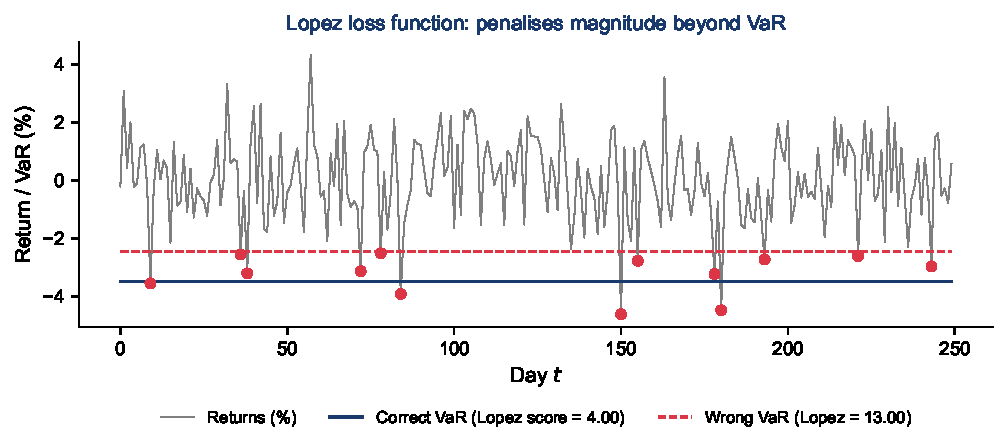
\includegraphics[width=\linewidth]{ch11_lopez_loss.pdf}\\[1pt]
{\scriptsize\textcolor{MediumGray}{\textit{VaR corect (albastru) -- scor mic. VaR gre\c sit (ro\c su) -- excep\c tii multiple \c si severe.}}}
\figql{SFM\_ch11\_lopez\_loss}{https://github.com/danpele/SFM/tree/main/Quantlets/Ch_11/SFM_ch11_lopez_loss}
\end{column}
\end{columns}
\end{cminipage}
\end{frame}

\slidelevel{PhD}
\begin{frame}{Berkowitz (2001): testul transform\u arii probabilistice}
\begin{cminipage}{0.96\textwidth}
\begin{block}{Idee: density forecast evaluation}
\begin{itemize}\setlength{\itemsep}{0pt}
    \item Sub densitatea prognozat\u a corect\u a $\hat f_t$:
    \[
        U_t = \hat F_t(r_t) \sim U(0,1)\quad\text{i.i.d.}
    \]
    \item Aplic\u a transformarea $z_t = \Phi^{-1}(U_t) \sim N(0,1)$ i.i.d.
    \item Test AR(1) cu medie: $z_t = \mu + \rho z_{t-1} + u_t$
    \item $H_0$: $\mu = 0$, $\rho = 0$, $\sigma_u^2 = 1$ $\Rightarrow$ $LR \sim \chi^2_3$
\end{itemize}
\end{block}
\begin{exampleblock}{Avantaje}
\begin{itemize}\setlength{\itemsep}{0pt}
    \item Folose\c ste \textbf{toat\u a} densitatea, nu doar coada (mai puternic ca Kupiec)
    \item Detecteaz\u a mismatch \^in toat\u a distribu\c tia
    \item Berkowitz \textbf{tail} -- variant\u a focalizat\u a doar pe $r_t < \VaR_t$
\end{itemize}
\end{exampleblock}
\end{cminipage}
\end{frame}

\slidelevel{Y3}
\begin{frame}{Distribu\c tia num\u arului de excep\c tii: vizualizare}
\begin{cminipage}{0.96\textwidth}
\begin{columns}[T]
\begin{column}{0.42\textwidth}
\begin{block}{Interpretare}
\begin{itemize}\setlength{\itemsep}{0pt}
    \item Sub $H_0$: $K \sim \text{Binomial}(n, \alpha)$
    \item Pentru $n=250$, $\alpha=5\%$: a\c steptat $12{,}5$, CI 95\% = $[6, 19]$
    \item Pentru $n=250$, $\alpha=1\%$: a\c steptat $2{,}5$, CI 95\% = $[0, 6]$
    \item Outside CI $\Rightarrow$ respingem $H_0$ Kupiec
\end{itemize}
\end{block}
\begin{exampleblock}{Aplica\c tie}
\begin{itemize}\setlength{\itemsep}{0pt}
    \item Dac\u a observ\u am $K = 18$ excep\c tii la $\alpha=5\%$: \^in CI $\Rightarrow$ model OK
    \item Dac\u a observ\u am $K = 12$ excep\c tii la $\alpha=1\%$: outside CI $\Rightarrow$ model rejected
\end{itemize}
\end{exampleblock}
\end{column}
\begin{column}{0.56\textwidth}
\centering
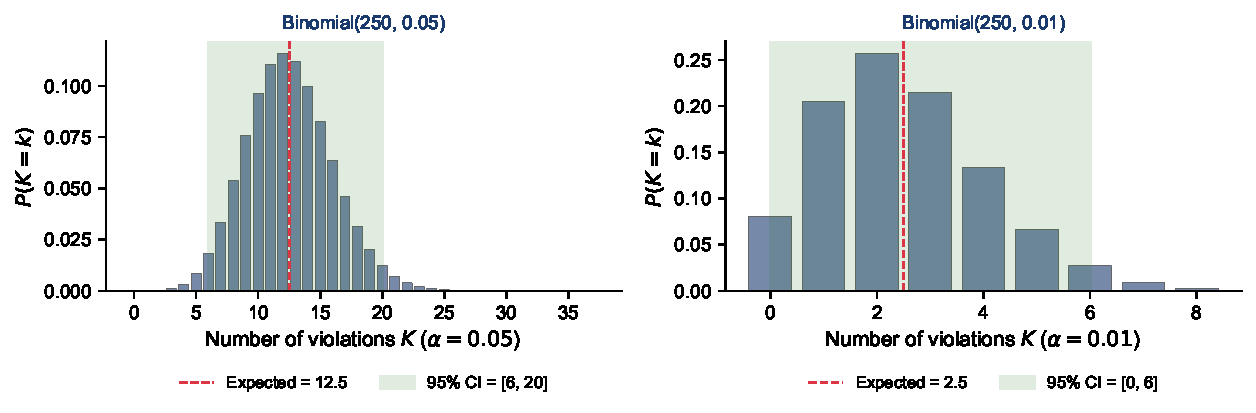
\includegraphics[width=\linewidth]{ch11_violation_dist.pdf}
\figql{SFM\_ch11\_violation\_dist}{https://github.com/danpele/SFM/tree/main/Quantlets/Ch_11/SFM_ch11_violation_dist}
\end{column}
\end{columns}
\end{cminipage}
\end{frame}

%#############################################################################
\section{Basel Traffic Light}
%#############################################################################

\slidelevel{Y3}
\begin{frame}{Basel Traffic Light: cadrul de reglementare}
\begin{cminipage}{0.95\textwidth}
\begin{block}{Cadrul Basel (1996, men\c tinut \c si \^in Basel III)}
\begin{itemize}\setlength{\itemsep}{0pt}
    \item Aplicat la VaR 99\% pe $n = 250$ zile de tranzac\c tionare
    \item Num\u arul de excep\c tii a\c steptate: $n\alpha = 2{,}5$
    \item Trei zone de decizie -- verde / galben / ro\c su (vezi tabelul)
\end{itemize}
\end{block}
\begin{center}
\renewcommand{\arraystretch}{1.25}
\small
\begin{tabular}{c c c c}
\toprule
\textbf{Zon\u a} & \textbf{Num\u ar excep\c tii} & \textbf{Multiplier add-on} & \textbf{Interpretare} \\
\midrule
\textcolor{Forest}{\textbf{Verde}}  & $0 \leq K \leq 4$  & $+0{,}00$ & Model acceptat \\
\textcolor{Amber}{\textbf{Galben}}  & $5 \leq K \leq 9$  & $+0{,}40$ -- $+0{,}85$ & Avertisment; investiga\c tie \\
\textcolor{Crimson}{\textbf{Ro\c su}} & $K \geq 10$        & $+1{,}00$ & Model respins; capital m\u arit \\
\bottomrule
\end{tabular}
\end{center}
\vspace{0.15cm}
\begin{itemize}\setlength{\itemsep}{0pt}
    \item Multiplier total: $m = 3 + \text{add-on}$; \textbf{capital de risc de pia\c t\u a} $= m \cdot \VaR$
    \item Probabilitatea sub $H_0$ (model corect) de a \textit{ateriza} \^in zona galben\u a: $\approx 5\%$
    \item Probabilitatea \^in zona ro\c sie: $\approx 0{,}01\%$ (rar\u a, dar costisitoare)
\end{itemize}
\end{cminipage}
\end{frame}

\slidelevel{Y3}
\begin{frame}{Distribu\c tia num\u arului de excep\c tii sub $H_0$}
\begin{cminipage}{0.96\textwidth}
\begin{columns}[T]
\begin{column}{0.45\textwidth}
\begin{itemize}\setlength{\itemsep}{1pt}
    \item $K \sim \text{Binomial}(n=250, \alpha=0{,}01)$
    \item Mod = $\lfloor 251 \cdot 0{,}01 \rfloor = 2$
    \item Media = $2{,}5$, abaterea standard $\approx 1{,}57$
    \item Probabilit\u a\c ti exacte:
    \begin{itemize}\setlength{\itemsep}{0pt}
        \item $\Pr(K \leq 4) = 89{,}2\%$
        \item $\Pr(5 \leq K \leq 9) = 10{,}8\%$
        \item $\Pr(K \geq 10) = 0{,}01\%$
    \end{itemize}
    \item \textbf{Probleme cu cadrul Basel}:
    \begin{itemize}\setlength{\itemsep}{0pt}
        \item Doar (P1); ignor\u a clustering-ul
        \item Penalizare asimetric\u a: subestimarea $>$ supraestimarea
    \end{itemize}
\end{itemize}
\end{column}
\begin{column}{0.52\textwidth}
\centering
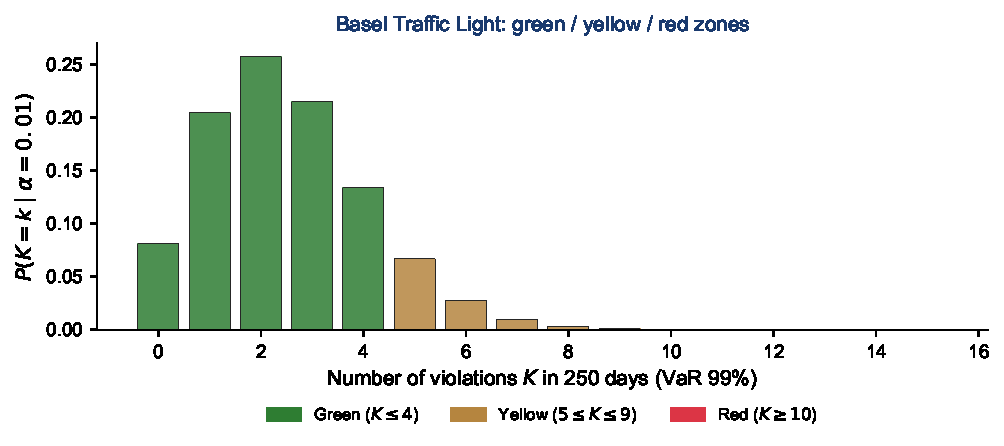
\includegraphics[width=\linewidth]{ch11_traffic_light.pdf}
\figql{SFM\_ch11\_traffic\_light}{https://github.com/danpele/SFM/tree/main/Quantlets/Ch_11/SFM_ch11_traffic_light}
\end{column}
\end{columns}
\end{cminipage}
\end{frame}

%#############################################################################
\section{Backtesting Expected Shortfall}
%#############################################################################

\slidelevel{MSc}
\begin{frame}{De ce e ES greu de backtestat?}
\begin{cminipage}{0.95\textwidth}
\begin{itemize}\setlength{\itemsep}{1pt}
    \item \textbf{Gneiting (2011)}: ES nu este \textit{elicitabil\u a} (nu exist\u a o func\c tie de scor strict\u a)
    \item \textbf{Consecin\c t\u a}: nu putem compara dou\u a prognoze ES prin scoring rules clasice
    \item Totu\c si, \textbf{ES este backtest-abil\u a} \^in sens larg (Acerbi--Szekely 2014)
    \item Trei abord\u ari moderne:
    \begin{enumerate}\setlength{\itemsep}{0pt}
        \item \textbf{Acerbi--Szekely 2014}: testele $Z_1$, $Z_2$, $Z_3$
        \item \textbf{Du--Escanciano 2017}: ESR (Expected Shortfall Regression)
        \item \textbf{Patton et al.\ 2019}: joint scoring VaR+ES
    \end{enumerate}
\end{itemize}

\vspace{0.15cm}

\begin{alertblock}{Note FRTB}
\begin{itemize}\setlength{\itemsep}{0pt}
    \item Cadrul Basel III FRTB nu cere backtest direct al ES
    \item Se backtesteaz\u a VaR 97{,}5\% \c si VaR 99\% \^in locul ES-ului
    \item Ipotez\u a implicit\u a: un model bun pentru VaR este bun \c si pentru ES
\end{itemize}
\end{alertblock}
\end{cminipage}
\end{frame}

\slidelevel{MSc}
\begin{frame}[shrink=22]{Acerbi--Szekely (2014): testele $Z_1$ \c si $Z_2$}
\begin{cminipage}{0.96\textwidth}
\begin{block}{$Z_1$: testul mediei \^in coad\u a}
\begin{itemize}\setlength{\itemsep}{0pt}
    \item Date: prognoze $\widehat{\VaR}_\alpha(t)$ \c si $\widehat{\ES}_\alpha(t)$, $t=1,\dots,T$
    \item Indicator de excep\c tie: $I_t = \mathbb{1}\{X_t < -\widehat{\VaR}_\alpha(t)\}$, $N_T = \sum_t I_t$
    \item Statistica:
    \[
        Z_1 = \frac{1}{N_T}\sum_{t=1}^{T} \frac{X_t \cdot I_t}{-\widehat{\ES}_\alpha(t)} + 1
    \]
    \item Sub $H_0$ (model corect): $\E[Z_1] = 0$
\end{itemize}
\end{block}

\begin{block}{$Z_2$: testul valorii totale pe coad\u a}
\begin{itemize}\setlength{\itemsep}{0pt}
    \item Statistica:
    \[
        Z_2 = \frac{1}{T \alpha}\sum_{t=1}^{T} \frac{X_t \cdot I_t}{-\widehat{\ES}_\alpha(t)} + 1
    \]
    \item Sub $H_0$: $\E[Z_2] = 0$
    \item Sub $H_1$ (model subestimeaz\u a coada): $Z_2 < 0$
\end{itemize}
\end{block}

\begin{itemize}\setlength{\itemsep}{0pt}
    \item Distribu\c tii sub $H_0$: estimate prin Monte Carlo (nu form\u a \^inchis\u a)
    \item \textbf{Avantaj}: condi\c tioneaz\u a pe model; sensibil la severitatea pierderilor extreme
\end{itemize}
\end{cminipage}
\end{frame}

\slidelevel{MSc}
\begin{frame}{$Z_2$ sub $H_0$ vs $H_1$ -- simulare}
\begin{cminipage}{0.96\textwidth}
\begin{columns}[T]
\begin{column}{0.55\textwidth}
\begin{itemize}\setlength{\itemsep}{1pt}
    \item Simulare $B = 4000$, $n = 250$, $\alpha = 5\%$
    \item \textbf{Verde ($H_0$)}: modelul Normal este corect $\Rightarrow$ $Z_2$ centrat \^in jurul lui 0
    \item \textbf{Ro\c su ($H_1$)}: adev\u arul este $t_4$ (cozi mai grele), dar modelul folosit este Normal\u a $\Rightarrow$ $Z_2$ deplasat negativ
    \item \textbf{Interpretare}: pierderile extreme realizate \textit{dep\u a\c sesc} ES-ul prognozat $\Rightarrow$ tail underestimated
    \item Critical value (5\% one-sided): $\approx -0{,}82$
\end{itemize}
\end{column}
\begin{column}{0.42\textwidth}
\centering
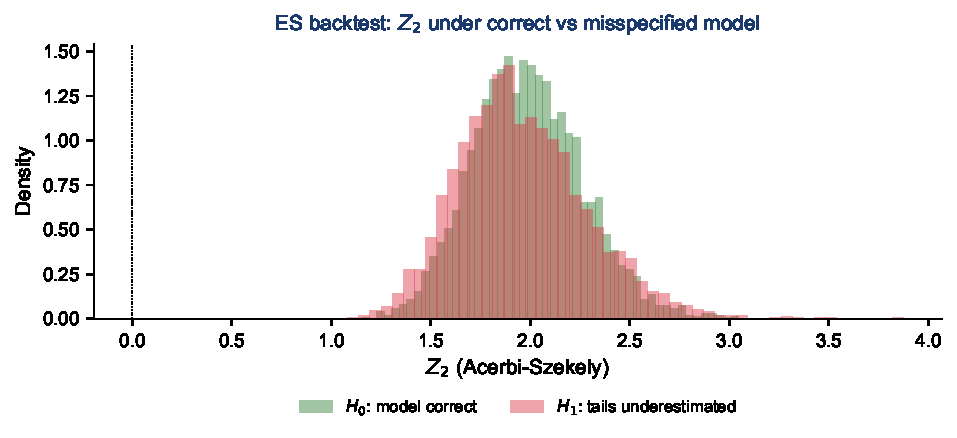
\includegraphics[width=\linewidth]{ch11_acerbi_szekely.pdf}
\figql{SFM\_ch11\_acerbi\_szekely}{https://github.com/danpele/SFM/tree/main/Quantlets/Ch_11/SFM_ch11_acerbi_szekely}
\end{column}
\end{columns}
\end{cminipage}
\end{frame}

%#############################################################################
\section{Studii de caz}
%#############################################################################

\slidelevel{Y3}
\begin{frame}{Studiu de caz 1: BVB (BET-like) cu \textit{jump} de criz\u a}
\begin{cminipage}{0.96\textwidth}
\begin{columns}[T]
\begin{column}{0.42\textwidth}
\begin{itemize}\setlength{\itemsep}{1pt}
    \item Date: 1500 zile simulate (proxy pentru BET 2017--2023)
    \item Volatility clustering pronun\c tat ($\beta = 0{,}87$)
    \item Cozi grele ($\nu = 5$)
    \item \textbf{Jump COVID-style}: $-8\%$ \^intr-o singur\u a zi
    \item Rolling HS-VaR/ES la $\alpha = 1\%$ cu $W = 250$
    \item \textbf{Observa\c tie}: dup\u a crash, VaR \textit{,,sare''} brusc \c si r\u am\^ane elevat \textbf{exact 250 zile} (ghost effect)
    \item \textbf{Concluzie practic\u a}: pentru pie\c te emergente cu jumps, HS singur\u a nu este suficient\u a; combina\c ti cu EVT \c si GARCH-VaR
\end{itemize}
\end{column}
\begin{column}{0.56\textwidth}
\centering
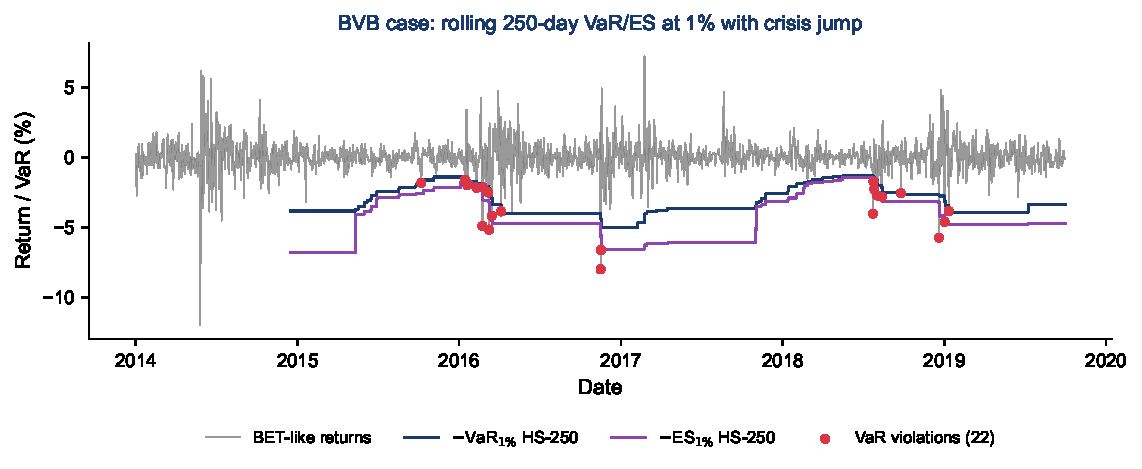
\includegraphics[width=\linewidth]{ch11_bvb_case.pdf}
\figql{SFM\_ch11\_bvb\_case}{https://github.com/danpele/SFM/tree/main/Quantlets/Ch_11/SFM_ch11_bvb_case}
\end{column}
\end{columns}
\end{cminipage}
\end{frame}

\slidelevel{MSc}
\begin{frame}{Studiu de caz 2: Lehman 2008 -- e\c secul VaR-ului gaussian}
\begin{cminipage}{0.96\textwidth}
\begin{columns}[T]
\begin{column}{0.42\textwidth}
\begin{itemize}\setlength{\itemsep}{1pt}
    \item 500 zile pre-criz\u a (vol $\sim 0{,}8\%$) + 60 zile de criz\u a (vol $\sim 3{,}5\%$ + jumps de $-9\%$)
    \item \textbf{VaR Normal\u a} (verde): subestimeaz\u a sever; multe excep\c tii \^in coad\u a
    \item \textbf{HS-VaR} (albastru): mai bun, dar tot insuficient -- vol pre-criz\u a domin\u a fereastra
    \item \textbf{Viol\u ari: Normal $\sim 25$, HS $\sim 12$} pe 60 zile de criz\u a (cu $\alpha = 1\% \Rightarrow$ a\c steptat 0{,}6)
    \item \textbf{Concluzie}: GARCH-VaR sau EVT-rolling sunt obligatorii \^in regim de criz\u a
\end{itemize}
\end{column}
\begin{column}{0.56\textwidth}
\centering
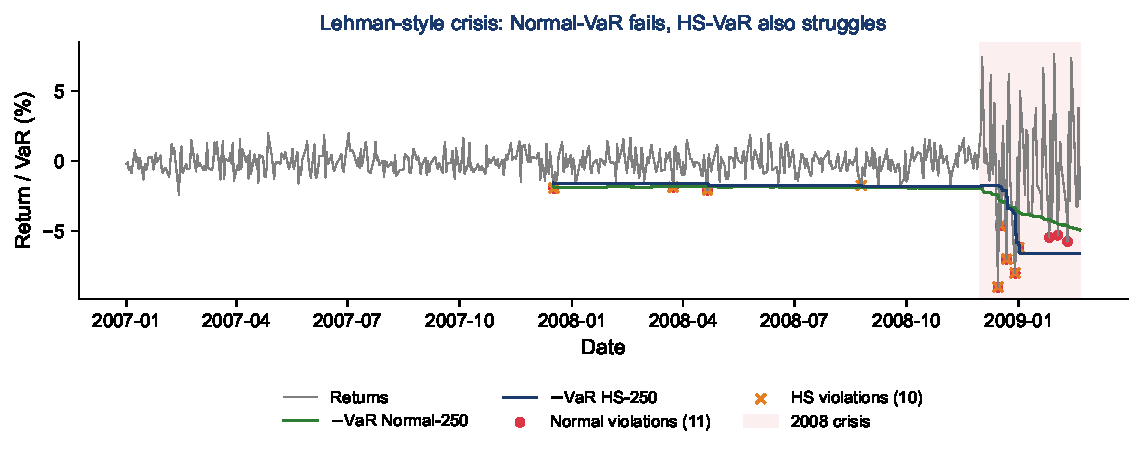
\includegraphics[width=\linewidth]{ch11_lehman_2008.pdf}
\figql{SFM\_ch11\_lehman\_2008}{https://github.com/danpele/SFM/tree/main/Quantlets/Ch_11/SFM_ch11_lehman_2008}
\end{column}
\end{columns}
\end{cminipage}
\end{frame}

\slidelevel{MSc}
\begin{frame}[shrink=10]{Lec\c tii din crizele istorice}
\begin{cminipage}{0.95\textwidth}
\renewcommand{\arraystretch}{1.2}
\begin{center}
\scriptsize
\begin{tabular}{llll}
\toprule
\textbf{Eveniment} & \textbf{Pierdere} & \textbf{Modele e\c suate} & \textbf{Lec\c tie} \\
\midrule
Black Monday 1987 & $-22{,}6\%$ S\&P 500 & Normal\u a, Black--Scholes & Cozi grele; $\sigma$ non-constant\u a \\
LTCM 1998 & \$4{,}6B pierdere & VaR backward-looking & Risc de coad\u a contagios \\
Dot-com 2000--02 & $-50\%$ NASDAQ & VaR sub regim bull & Schimb\u ari structurale \\
Subprime 2007--09 & Lehman, AIG falimente & Copule gaussiene, VaR & Cozi \^in dependen\c t\u a \\
Flash Crash 2010 & $-9\%$ \^in 5 minute & Modele de lichiditate & Intraday VaR; microstructur\u a \\
COVID 2020 & $-12\%$ \^intr-o zi DJI & VaR rolling W=250 & Adaptare rapid\u a la regim \\
SVB 2023 & Falimente bancare & VaR ratei dob\^anzii & Duration risk + bank run \\
\bottomrule
\end{tabular}
\end{center}
\vspace{0.2cm}
\begin{alertblock}{Pattern comun}
\begin{itemize}\setlength{\itemsep}{0pt}
    \item \^In toate cazurile: VaR pre-criz\u a $\ll$ pierderea realizat\u a
    \item Viol\u ari clusterizate $\Rightarrow$ e\c sec Christoffersen IC
\end{itemize}
\end{alertblock}
\end{cminipage}
\end{frame}

\slidelevel{Y3}
\begin{frame}{Studiu de caz 3: cripto -- crashul FTX (noiembrie 2022)}
\begin{cminipage}{0.96\textwidth}
\begin{columns}[T]
\begin{column}{0.42\textwidth}
\begin{itemize}\setlength{\itemsep}{0pt}
    \item Date: 800 zile simulate (proxy BTC 2020--2023)
    \item Volatilitate ridicat\u a ($\sigma \approx 3\%$ zilnic)
    \item Eveniment FTX: $-20\%$ \^intr-o singur\u a zi, urmat de runs
    \item Rolling HS-VaR la $\alpha = 1\%$, $W = 250$
\end{itemize}
\begin{alertblock}{Observa\c tii}
\begin{itemize}\setlength{\itemsep}{0pt}
    \item VaR pre-criz\u a $\sim 8\%$; pierderea $\sim 20\%$
    \item Viol\u ari clusterizate: peste 10 \^in 30 zile
    \item Crypto cere modele dedicate (jumps, switching)
\end{itemize}
\end{alertblock}
\end{column}
\begin{column}{0.56\textwidth}
\centering
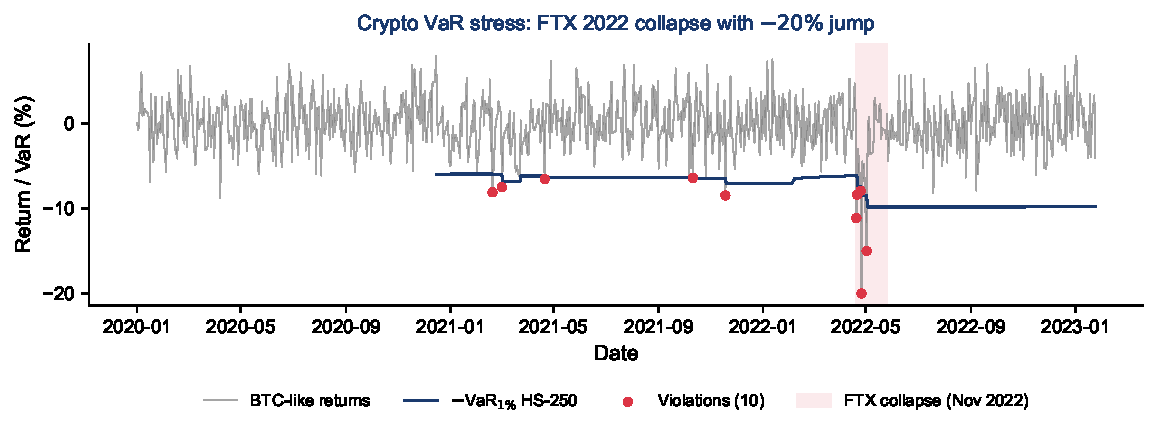
\includegraphics[width=\linewidth]{ch11_crypto_var.pdf}
\figql{SFM\_ch11\_crypto\_var}{https://github.com/danpele/SFM/tree/main/Quantlets/Ch_11/SFM_ch11_crypto_var}
\end{column}
\end{columns}
\end{cminipage}
\end{frame}

\slidelevel{MSc}
\begin{frame}{Studiu de caz 4: VaR cross-asset (FX, equity, credit, commodities)}
\begin{cminipage}{0.96\textwidth}
\begin{columns}[T]
\begin{column}{0.40\textwidth}
\begin{itemize}\setlength{\itemsep}{0pt}
    \item Compara\c tie VaR 1\% pe 7 clase de active
    \item \textbf{Cripto} (BTC) -- cel mai volatil ($\sigma \sim 4\%$, $\nu \sim 3{,}5$)
    \item \textbf{Oil} -- vol mare, cozi grele ($\nu = 4$)
    \item \textbf{Equity} (S\&P, BET) -- moderate
    \item \textbf{Bonds IG} -- vol mic\u a, cozi aproape Normale
    \item \textbf{Gap} Student-$t$ vs Normal\u a cre\c ste cu cozile (BTC: $+40\%$, Bonds: $+5\%$)
\end{itemize}
\end{column}
\begin{column}{0.58\textwidth}
\centering
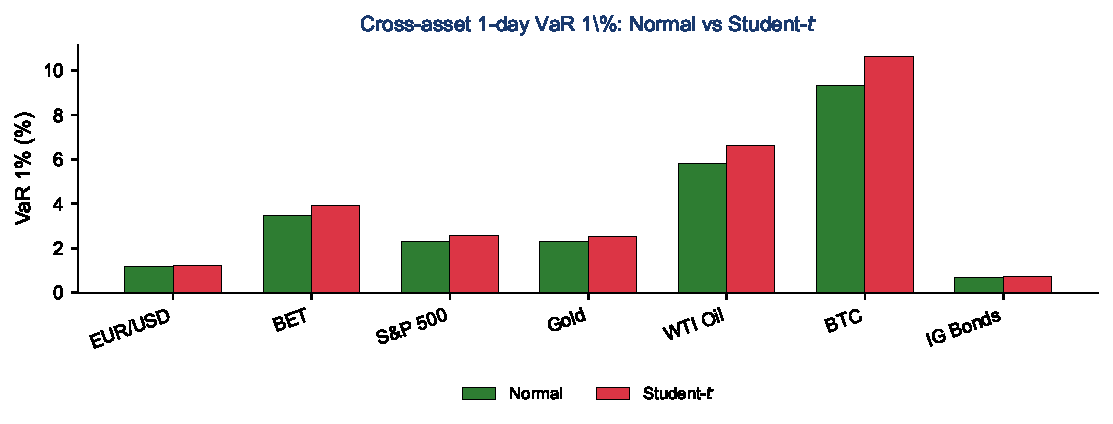
\includegraphics[width=\linewidth]{ch11_cross_asset.pdf}
\figql{SFM\_ch11\_cross\_asset}{https://github.com/danpele/SFM/tree/main/Quantlets/Ch_11/SFM_ch11_cross_asset}
\end{column}
\end{columns}
\end{cminipage}
\end{frame}

\slidelevel{MSc}
\begin{frame}{Studiu de caz 5: Russia 2022 \c si sanc\c tiunile (FX VaR shock)}
\begin{cminipage}{0.96\textwidth}
\begin{itemize}\setlength{\itemsep}{1pt}
    \item \textbf{Februarie 2022}: invazia Ucrainei + sanc\c tiuni occidentale
    \item RUB/USD a c\u azut $40\%$ \^in 2 s\u apt\u am\^ani
    \item Multe trad. desks foloseau VaR Normal pe FX -- subestimare masiv\u a
    \item Capital ce trebuia (real) vs.\ capital alocat: raport $5\times$--$10\times$
    \item \textbf{Lec\c tie}:
    \begin{itemize}\setlength{\itemsep}{0pt}
        \item VaR ignor\u a riscul \textbf{geopolitic} (event-driven)
        \item Solu\c tie: scenario VaR + jump-diffusion + Stressed VaR Basel III
    \end{itemize}
    \item \textbf{Impact pe banci RO/EU}: Raiffeisen, UniCredit etc.\ -- impairments majore
\end{itemize}
\vspace{0.15cm}
\begin{alertblock}{Lec\c tie practic\u a}
\begin{itemize}\setlength{\itemsep}{0pt}
    \item Niciun model VaR clasic nu poate prognoza un \textbf{regime shift geopolitic}
    \item Stress testing + reverse stress testing sunt obligatorii (BCBS 2022)
\end{itemize}
\end{alertblock}
\end{cminipage}
\end{frame}

\slidelevel{MSc}
\begin{frame}{Studiu de caz 6: SVB 2023 -- riscul de rata dob\^anzii}
\begin{cminipage}{0.96\textwidth}
\begin{itemize}\setlength{\itemsep}{1pt}
    \item \textbf{Martie 2023}: Silicon Valley Bank colaps \^in 48 ore
    \item Cauza prim\u a: portofoliu de Treasuries \textbf{HTM} la dob\^anzi mici (1\%); cre\c sterea Fed-rate la 5\%
    \item Pierdere de market value pe HTM: \$15 mld neraportat\u a \^in VaR
    \item \textbf{De ce VaR a e\c suat}:
    \begin{itemize}\setlength{\itemsep}{0pt}
        \item Treasuries HTM erau \textbf{exclu\c si} din trading book (\c si din VaR)
        \item Risk management nu acoperea \textbf{duration risk} pe banking book
        \item Concentrare clien\c ti (tech startups) $\Rightarrow$ bank run digital
    \end{itemize}
    \item \textbf{Reforme post-SVB}:
    \begin{itemize}\setlength{\itemsep}{0pt}
        \item Includerea unrealised AOCI \^in capital reglementar (Basel)
        \item Stress testing pe regime de dob\^and\u a (CCAR enhancements)
        \item LCR enhanced pentru concentr\u ari de depozite
    \end{itemize}
\end{itemize}
\end{cminipage}
\end{frame}

%#############################################################################
\section{Recomand\u ari practice \c si FRTB}
%#############################################################################

\slidelevel{Y3}
\begin{frame}{Recomand\u ari practice pentru risk manager}
\begin{cminipage}{0.95\textwidth}
\begin{enumerate}\setlength{\itemsep}{2pt}
    \item \textbf{Nu raporta\c ti niciodat\u a un singur model}: combina\c ti HS + GARCH-$t$ + EVT pentru cuantile extreme
    \item \textbf{Raporta\c ti ES al\u aturi de VaR}: ES surprinde severitatea, VaR doar pragul
    \item \textbf{Backtest complet}: Kupiec POF + Christoffersen CC + Engle--Manganelli DQ
    \item \textbf{Stress testing complementar}: scenarii istorice (1987, 2008, COVID) + scenarii ipotetice
    \item \textbf{Aten\c tie la regim shifts}: monitoriza\c ti volatilitatea condi\c tional\u a (GARCH, RealVol)
    \item \textbf{Ferestre multiple}: $W \in \{250, 500, 1000\}$ pentru robuste\c te
    \item \textbf{Documenta\c ti ipotezele}: distribu\c tie, orizont, fereastr\u a, surse de date
    \item \textbf{Sanity checks}: raportul ES/VaR ar trebui s\u a fie $\sim 1{,}2$ (Normal) p\^an\u a la $\sim 1{,}5$ (cozi foarte grele)
\end{enumerate}
\vspace{0.1cm}
\begin{exampleblock}{Regula de aur (Jorion 2007)}
\begin{itemize}\setlength{\itemsep}{0pt}
    \item \textit{,,No risk model survives contact with the market.''}
    \item Cel mai important \textbf{nu} este alegerea modelului perfect
    \item Ci \textbf{monitorizarea continu\u a} \c si \textbf{actualizarea} atunci c\^and modelul e\c sueaz\u a backtesting-ul
\end{itemize}
\end{exampleblock}
\end{cminipage}
\end{frame}

\slidelevel{MSc}
\begin{frame}{FRTB: noul standard regulator (2023+)}
\begin{cminipage}{0.95\textwidth}
\begin{block}{Fundamental Review of the Trading Book (BCBS)}
\begin{itemize}\setlength{\itemsep}{1pt}
    \item \^Inlocuie\c ste VaR cu \textbf{Expected Shortfall 97{,}5\%} ca m\u asur\u a principal\u a
    \item \textbf{Stressed calibration}: estimat\u a pe perioada cea mai stresant\u a de 12 luni din ultimii 10 ani
    \item \textbf{Orizonturi diferen\c tiate de lichiditate}:
    \begin{itemize}\setlength{\itemsep}{0pt}
        \item 10 zile -- ac\c tiuni mari, FX major
        \item 20 zile -- ac\c tiuni mici-medii, credit IG
        \item 40 zile -- credit speculativ
        \item 60 / 120 zile -- pia\c te exotice / iliquide
    \end{itemize}
    \item \textbf{IMA (Internal Models Approach)}: necesit\u a aprobare per desk (nu mai global)
    \item \textbf{P\&L Attribution test}: alinierea P\&L \textit{hypothetical} cu \textit{actual} -- nou hurdle
\end{itemize}
\end{block}
\vspace{0.15cm}
\begin{itemize}\setlength{\itemsep}{0pt}
    \item \textbf{Implementare \^in UE}: CRR3 (\^in vigoare 2025)
    \item \textbf{Rom\^ania}: BNR aplic\u a direct CRR3 pentru institu\c tiile mari (Banca Transilvania, BCR, Raiffeisen, etc.)
\end{itemize}
\end{cminipage}
\end{frame}

\slidelevel{Y3}
\begin{frame}{Arbore de decizie: ce metod\u a VaR s\u a aleg?}
\begin{cminipage}{0.98\textwidth}
\begin{center}
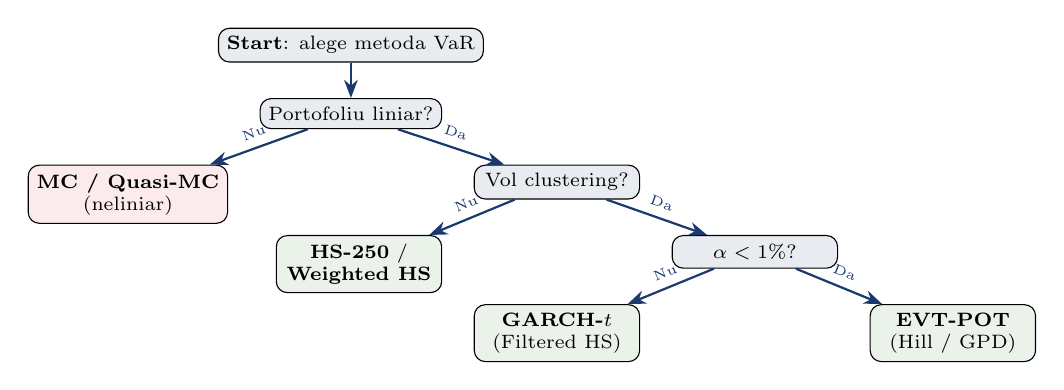
\begin{tikzpicture}[
    node distance=0.45cm and 0.4cm,
    every node/.style={font=\scriptsize},
    box/.style={draw, rounded corners, fill=MainBlue!10, align=center,
                inner sep=3pt, minimum width=2.1cm},
    rbox/.style={draw, rounded corners, fill=Crimson!10, align=center,
                 inner sep=3pt, minimum width=2.1cm},
    gbox/.style={draw, rounded corners, fill=Forest!10, align=center,
                 inner sep=3pt, minimum width=2.1cm},
    arrow/.style={->, >=Stealth, thick, color=MainBlue}]

\node[box] (start) {\textbf{Start}: alege metoda VaR};
\node[box, below=of start] (q1) {Portofoliu liniar?};
\node[rbox, below left=of q1] (mc) {\textbf{MC / Quasi-MC}\\(neliniar)};
\node[box, below right=of q1] (q2) {Vol clustering?};
\node[gbox, below left=of q2] (hs) {\textbf{HS-250} /\\\textbf{Weighted HS}};
\node[box, below right=of q2] (q3) {$\alpha < 1\%$?};
\node[gbox, below left=of q3] (garch) {\textbf{GARCH-$t$}\\(Filtered HS)};
\node[gbox, below right=of q3] (evt) {\textbf{EVT-POT}\\(Hill / GPD)};

\draw[arrow] (start) -- (q1);
\draw[arrow] (q1) -- (mc) node[midway, above, sloped] {\tiny Nu};
\draw[arrow] (q1) -- (q2) node[midway, above, sloped] {\tiny Da};
\draw[arrow] (q2) -- (hs) node[midway, above, sloped] {\tiny Nu};
\draw[arrow] (q2) -- (q3) node[midway, above, sloped] {\tiny Da};
\draw[arrow] (q3) -- (garch) node[midway, above, sloped] {\tiny Nu};
\draw[arrow] (q3) -- (evt) node[midway, above, sloped] {\tiny Da};
\end{tikzpicture}
\end{center}
\vspace{0.15cm}
\begin{itemize}\setlength{\itemsep}{0pt}
    \item \^Intotdeauna raporta\c ti \textbf{cel pu\c tin dou\u a} metode pentru cross-validation
    \item Backtesting Kupiec + Christoffersen + DQ pe toate cele alese
\end{itemize}
\end{cminipage}
\end{frame}

\slidelevel{MSc}
\begin{frame}[shrink=10]{Liquidity-adjusted VaR (LVaR): adaug\u a costul de lichiditate}
\begin{cminipage}{0.96\textwidth}
\begin{columns}[T]
\begin{column}{0.50\textwidth}
\begin{block}{Formul\u a (Bangia et al.\ 1999)}
\begin{itemize}\setlength{\itemsep}{0pt}
    \item VaR standard ignor\u a costurile de lichidare
    \item LVaR adaug\u a half-spread + market impact:
    \[
        \text{LVaR}_\alpha = \VaR_\alpha + \tfrac{1}{2}(s + k\sigma_s)
    \]
    \item $s$ = spread mediu, $\sigma_s$ = vol spread-ului, $k$ = cuantila
    \item Modele moderne: \^impart liquidation \^in zile multiple
\end{itemize}
\end{block}
\begin{exampleblock}{C\^and conteaz\u a}
\begin{itemize}\setlength{\itemsep}{0pt}
    \item \textbf{Cripto}, ac\c tiuni small-cap, FX exotic
    \item Portofolii mari relativ la pia\c t\u a (LTCM-style)
    \item Crize de lichiditate (2008, 2020 March)
\end{itemize}
\end{exampleblock}
\end{column}
\begin{column}{0.46\textwidth}
\centering
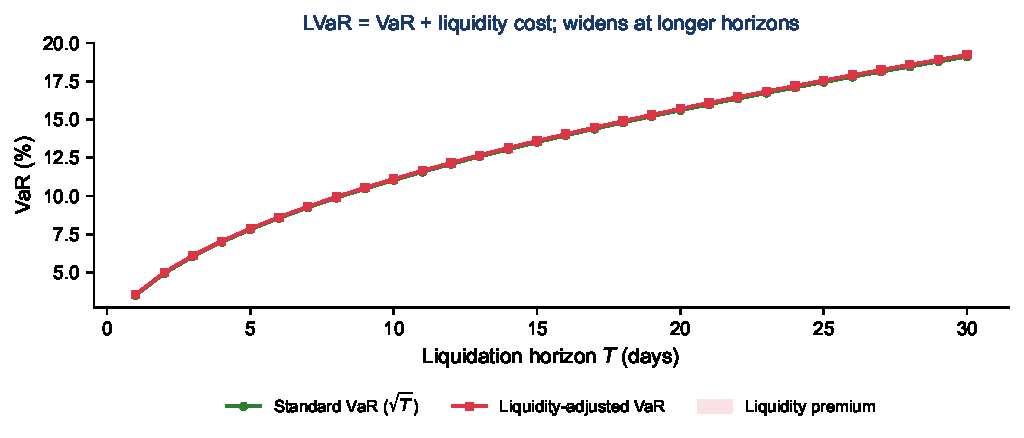
\includegraphics[width=\linewidth]{ch11_lvar.pdf}\\[1pt]
{\scriptsize\textcolor{MediumGray}{\textit{LVaR (Crimson) dep\u a\c se\c ste VaR standard (Forest); diferen\c ta cre\c ste cu orizontul.}}}
\figql{SFM\_ch11\_lvar}{https://github.com/danpele/SFM/tree/main/Quantlets/Ch_11/SFM_ch11_lvar}
\end{column}
\end{columns}
\end{cminipage}
\end{frame}

\slidelevel{MSc}
\begin{frame}[shrink=10]{VaR pentru op\c tiuni: delta-gamma vs full reval}
\begin{cminipage}{0.96\textwidth}
\begin{block}{Aproximarea delta (linear)}
\begin{itemize}\setlength{\itemsep}{0pt}
    \item Pentru op\c tiuni cu mi\c sc\u ari mici: $\Delta V \approx \Delta \cdot \Delta S$
    \item $\VaR^{delta}_\alpha = |\Delta| \cdot S \cdot \sigma \cdot |z_\alpha|$
    \item \textbf{Eroare}: subestimeaz\u a riscul pentru mi\c sc\u ari mari
\end{itemize}
\end{block}
\begin{block}{Delta-Gamma (corec\c tie Cornish-Fisher style)}
\begin{itemize}\setlength{\itemsep}{0pt}
    \item Adaug\u a termenul $\Gamma$: $\Delta V \approx \Delta\cdot\Delta S + \tfrac{1}{2}\Gamma(\Delta S)^2$
    \item Distribu\c tia P\&L: skewness + kurtoz\u a $\Rightarrow$ Cornish-Fisher
\end{itemize}
\end{block}
\begin{alertblock}{Full revaluation (Monte Carlo)}
\begin{itemize}\setlength{\itemsep}{0pt}
    \item Genereaz\u a $M$ scenarii ale $S$, reprice op\c tiunea complet (Black-Scholes / binomial)
    \item Cel mai precis dar costisitor (necesar pentru op\c tiuni exotice: barrier, Asian)
    \item Folosit \^in industrie pentru op\c tiuni cu $\Gamma$ mare sau op\c tiuni cu barier\u a
\end{itemize}
\end{alertblock}
\end{cminipage}
\end{frame}

%-----------------------------------------------------------------------------
% Quiz formativ
%-----------------------------------------------------------------------------

\slidelevel{Y3}
\begin{frame}{Quiz formativ -- VaR \c si ES (1/3)}
\begin{cminipage}{0.96\textwidth}
\begin{enumerate}\setlength{\itemsep}{3pt}
    \item<1-> Sub Normal\u a cu $\mu = 0$, $\sigma = 1\%$, c\^at este $\VaR_{1\%}$?
    \begin{itemize}\setlength{\itemsep}{0pt}
        \item A) $1{,}00\%$
        \item B) $1{,}65\%$
        \item C) $2{,}33\%$ \onslide<2->{\textbf{$\leftarrow$ r\u aspuns}}
        \item D) $2{,}58\%$
    \end{itemize}
    \item<3-> Care afirma\c tie despre ES este \textbf{fals\u a}?
    \begin{itemize}\setlength{\itemsep}{0pt}
        \item A) ES $\geq$ VaR
        \item B) ES este subaditiv\u a
        \item C) ES are formul\u a \^inchis\u a sub Normal\u a
        \item D) ES poate fi mai mic\u a dec\^at VaR \onslide<4->{\textbf{$\leftarrow$ r\u aspuns}}
    \end{itemize}
\end{enumerate}
\onslide<5->{\begin{block}{Sumar r\u aspunsuri}1-C ($\sigma \cdot |z_{0,01}| = 0{,}01 \cdot 2{,}326 \approx 2{,}33\%$); 2-D (ES $\geq$ VaR mereu)\end{block}}
\end{cminipage}
\end{frame}

\slidelevel{Y3}
\begin{frame}{Quiz formativ -- backtesting (2/3)}
\begin{cminipage}{0.96\textwidth}
\begin{enumerate}\setlength{\itemsep}{3pt}
    \item<1-> Testul Kupiec POF testeaz\u a:
    \begin{itemize}\setlength{\itemsep}{0pt}
        \item A) Frecven\c ta excep\c tiilor \onslide<2->{\textbf{$\leftarrow$ r\u aspuns}}
        \item B) Independen\c ta excep\c tiilor
        \item C) Magnitudinea excep\c tiilor
        \item D) Severitatea cozii
    \end{itemize}
    \item<3-> \^In zona ro\c sie Basel ($K \geq 10$ pentru VaR 99\%, $n=250$):
    \begin{itemize}\setlength{\itemsep}{0pt}
        \item A) Capital reglementar nemodificat
        \item B) Multiplier add-on $+0{,}40$
        \item C) Multiplier add-on $+1{,}00$, model respins \onslide<4->{\textbf{$\leftarrow$ r\u aspuns}}
        \item D) Doar avertisment, f\u ar\u a impact capital
    \end{itemize}
\end{enumerate}
\onslide<5->{\begin{block}{Sumar}1-A; 2-C (zona ro\c sie cere model nou + capital m\u arit)\end{block}}
\end{cminipage}
\end{frame}

\slidelevel{MSc}
\begin{frame}{Quiz formativ -- metode \c si reglementare (3/3)}
\begin{cminipage}{0.96\textwidth}
\begin{enumerate}\setlength{\itemsep}{3pt}
    \item<1-> FRTB (Basel III final) folose\c ste:
    \begin{itemize}\setlength{\itemsep}{0pt}
        \item A) VaR 99\%
        \item B) Expected Shortfall 97{,}5\% \onslide<2->{\textbf{$\leftarrow$ r\u aspuns}}
        \item C) Stressed VaR doar
        \item D) Median Shortfall
    \end{itemize}
    \item<3-> Pentru cuantile extreme ($\alpha = 0{,}1\%$) pe ac\c tiuni emergente, recomandarea cea mai bun\u a:
    \begin{itemize}\setlength{\itemsep}{0pt}
        \item A) HS-250
        \item B) Normal\u a parametric\u a
        \item C) EVT-POT cu Student-$t$ inova\c tii \onslide<4->{\textbf{$\leftarrow$ r\u aspuns}}
        \item D) Monte Carlo cu $M=10^4$
    \end{itemize}
\end{enumerate}
\onslide<5->{\begin{block}{Sumar}1-B; 2-C (EVT este standard pentru cuantile extreme)\end{block}}
\end{cminipage}
\end{frame}

\slidelevel{Y3}
\begin{frame}[shrink=20]{Exerci\c tii de examen (rezolvate)}
\begin{cminipage}{0.96\textwidth}
\begin{block}{Exerci\c tiu 1: VaR Normal\u a pe portofoliu}
\begin{itemize}\setlength{\itemsep}{0pt}
    \item Portofoliu $V = 5$ mil EUR, $r \sim \mathcal{N}(0, 0{,}012^2)$
    \item $\VaR_{99\%}^{1d} = -V(\mu + \sigma z_{0,01}) = 5 \cdot 0{,}012 \cdot 2{,}326 = 0{,}14$ mil EUR
    \item $\VaR_{99\%}^{10d} = 0{,}14 \cdot \sqrt{10} = 0{,}44$ mil EUR (regula $\sqrt{T}$)
    \item Capital Basel = $3 \cdot 0{,}44 = 1{,}32$ mil EUR
\end{itemize}
\end{block}
\begin{block}{Exerci\c tiu 2: backtesting Kupiec}
\begin{itemize}\setlength{\itemsep}{0pt}
    \item Date: $n = 250$ zile, $\alpha = 5\%$, observat $x = 18$ excep\c tii
    \item $\hat p = 18/250 = 0{,}072$
    \item $LR_{POF} = -2[18\ln(0{,}05/0{,}072) + 232\ln(0{,}95/0{,}928)] = 2{,}43$
    \item $p$-value $= 0{,}119 > 0{,}05$ $\Rightarrow$ nu respingem $H_0$
\end{itemize}
\end{block}
\begin{block}{Exerci\c tiu 3: ES Normal\u a vs Student-$t$}
\begin{itemize}\setlength{\itemsep}{0pt}
    \item $\sigma = 1\%$, $\alpha = 1\%$
    \item $\ES_{1\%}^{N} = 1\% \cdot \phi(-2{,}326)/0{,}01 = 2{,}67\%$
    \item $\ES_{1\%}^{t_5} = 3{,}20\%$ ($\sim 20\%$ mai mare)
\end{itemize}
\end{block}
\end{cminipage}
\end{frame}

%#############################################################################
\section{Concluzii \c si referin\c te}
%#############################################################################

\slidelevel{MSc}
\begin{frame}[shrink=10]{Tabel sintetic: compararea celor 6 metode}
\begin{cminipage}{0.97\textwidth}
\renewcommand{\arraystretch}{1.25}
\begin{center}
\footnotesize
\begin{tabular}{l c c c c}
\toprule
\textbf{Metod\u a} & \textbf{Cozi grele} & \textbf{Vol clustering} & \textbf{Cuantile extreme} & \textbf{Cost} \\
\midrule
HS-250 & \textcolor{Forest}{partial} & \textcolor{Crimson}{slab} & \textcolor{Crimson}{limitat la $1/W$} & \textcolor{Forest}{mic} \\
Weighted HS & \textcolor{Forest}{partial} & \textcolor{Amber}{moderat} & \textcolor{Crimson}{limitat} & \textcolor{Forest}{mic} \\
Parametric Normal\u a & \textcolor{Crimson}{NU} & \textcolor{Crimson}{NU} & \textcolor{Crimson}{subestimeaz\u a} & \textcolor{Forest}{$O(1)$} \\
Parametric $t$ / skew-$t$ & \textcolor{Forest}{DA} & \textcolor{Crimson}{NU} & \textcolor{Amber}{moderat} & \textcolor{Forest}{$O(1)$} \\
Cornish-Fisher & \textcolor{Amber}{moderat} & \textcolor{Crimson}{NU} & \textcolor{Crimson}{NU pentru $\alpha<1\%$} & \textcolor{Forest}{$O(1)$} \\
Monte Carlo & \textcolor{Forest}{DA (dac\u a model corect)} & \textcolor{Forest}{DA (cond.)} & \textcolor{Forest}{DA (cu IS)} & \textcolor{Crimson}{$O(M)$} \\
GARCH-VaR & \textcolor{Amber}{depinde de inova\c tie} & \textcolor{Forest}{\textbf{DA}} & \textcolor{Amber}{moderat} & \textcolor{Amber}{$O(T)$ fit} \\
Filtered HS & \textcolor{Forest}{\textbf{DA}} & \textcolor{Forest}{\textbf{DA}} & \textcolor{Forest}{DA} & \textcolor{Amber}{$O(T)$} \\
EVT-POT (GPD) & \textcolor{Forest}{\textbf{DA (designed for)}} & \textcolor{Crimson}{NU (default)} & \textcolor{Forest}{\textbf{DA}} & \textcolor{Amber}{$O(T)$ + alegere prag} \\
\bottomrule
\end{tabular}
\end{center}
\vspace{0.15cm}
\begin{exampleblock}{Stack recomandat \^in produc\c tie (Basel-grade)}
\begin{itemize}\setlength{\itemsep}{0pt}
    \item \textbf{Strat 1} (zilnic): HS-250 -- benchmark non-parametric
    \item \textbf{Strat 2} (zilnic): GARCH(1,1)-$t$ sau Filtered HS -- adaptare la regim
    \item \textbf{Strat 3} (s\u apt\u am\^anal): EVT-POT pentru $\alpha = 0{,}1\%$ -- tail risk
    \item \textbf{Backtest}: Kupiec + Christoffersen + DQ + Acerbi-Szekely pe ES
\end{itemize}
\end{exampleblock}
\end{cminipage}
\end{frame}

\slidelevel{MSc}
\begin{frame}[shrink=10]{Pa\c si practici pentru implementarea unui sistem VaR}
\begin{cminipage}{0.96\textwidth}
\begin{enumerate}\setlength{\itemsep}{1pt}
    \item[\textcolor{MainBlue}{\textbf{1.}}] \textbf{Inventory portofoliu}: identific\u a toate pozi\c tiile, factori de risc, mapeaz\u a la time series
    \item[\textcolor{MainBlue}{\textbf{2.}}] \textbf{Date}: surse oficiale (Bloomberg, Refinitiv), QC pe valori aberante (\textit{outliers}), interpolare goluri (\textit{gap filling})
    \item[\textcolor{MainBlue}{\textbf{3.}}] \textbf{Alege metoda}: aplica\c ti arborele de decizie din slide-ul anterior
    \item[\textcolor{MainBlue}{\textbf{4.}}] \textbf{Implementa\c ti}: \texttt{numpy/pandas} + \texttt{arch} pentru GARCH + \texttt{scipy} pentru fit
    \item[\textcolor{MainBlue}{\textbf{5.}}] \textbf{Validare \^in oglind\u a (parallel run)}: 6 luni rolling vs.\ sistemul anterior
    \item[\textcolor{MainBlue}{\textbf{6.}}] \textbf{Backtesting riguros}: Kupiec POF + Christoffersen IC/CC + DQ
    \item[\textcolor{MainBlue}{\textbf{7.}}] \textbf{Reporting zilnic}: VaR + ES + 3 metode + traffic light + violations
    \item[\textcolor{MainBlue}{\textbf{8.}}] \textbf{Stress testing complementar}: scenarii istorice + ipotetice + reverse stress
    \item[\textcolor{MainBlue}{\textbf{9.}}] \textbf{Governance}: comitet de risc s\u apt\u am\^anal, escalare automate
    \item[\textcolor{MainBlue}{\textbf{10.}}] \textbf{Audit anual}: model validation independent, documenta\c tie complet\u a (Basel SR 11-7)
\end{enumerate}
\vspace{0.15cm}
\begin{alertblock}{Sucesul depinde de}
\begin{itemize}\setlength{\itemsep}{0pt}
    \item \textbf{Date} (60\% din valoare) $>$ \textbf{Model} (30\%) $>$ \textbf{Infrastructur\u a} (10\%)
\end{itemize}
\end{alertblock}
\end{cminipage}
\end{frame}

\slidelevel{Y3}
\begin{frame}[shrink=15]{Glosar tehnic: principalele formule}
\begin{cminipage}{0.96\textwidth}
\footnotesize
\begin{itemize}\setlength{\itemsep}{1pt}
    \item $\VaR_\alpha = \inf\{\ell : \Pr(L > \ell) \leq \alpha\} = -F_X^{-1}(\alpha)$
    \item $\ES_\alpha = \E[L \mid L \geq \VaR_\alpha] = \tfrac{1}{\alpha}\int_0^\alpha \VaR_u\, du$
    \item \textbf{VaR Normal\u a}: $-(\mu + \sigma z_\alpha)$, cu $z_\alpha = \Phi^{-1}(\alpha)$
    \item \textbf{ES Normal\u a}: $-\mu + \sigma \phi(z_\alpha)/\alpha$
    \item \textbf{VaR Student-$t$}: $-(\mu + \sigma\sqrt{(\nu-2)/\nu}\cdot t_\nu^{-1}(\alpha))$
    \item \textbf{GARCH(1,1)}: $\sigma_t^2 = \omega + \alpha\varepsilon_{t-1}^2 + \beta\sigma_{t-1}^2$
    \item \textbf{GPD}: $1 - (1+\xi y/\beta)^{-1/\xi}$, $y > 0$
    \item \textbf{VaR POT}: $u + (\beta/\xi)\big((n/N_u\cdot\alpha)^{-\xi}-1\big)$
    \item \textbf{ES POT}: $\VaR/(1-\xi) + (\beta-\xi u)/(1-\xi)$
    \item \textbf{Hill estim.}: $\hat\xi_H = \tfrac{1}{k}\sum_{i=1}^k \ln(L_{(i)}/L_{(k+1)})$
    \item \textbf{Kupiec POF}: $LR = -2\ln[\alpha^x(1-\alpha)^{n-x}/\hat p^x(1-\hat p)^{n-x}] \sim \chi^2_1$
    \item \textbf{Christoffersen IC}: $LR_{IC} = LR_{CC} - LR_{POF} \sim \chi^2_1$
    \item \textbf{Lopez score}: $\sum_t [1 + (r_t+\VaR_t)^2]\cdot\mathbb{1}\{r_t<-\VaR_t\}$
    \item \textbf{Acerbi-Szekely $Z_2$}: $\tfrac{1}{T\alpha}\sum_t\tfrac{r_t I_t}{-\ES_t} + 1$
    \item \textbf{Cornish-Fisher}: $z^{CF}_\alpha = z_\alpha + (z_\alpha^2-1)S/6 + \ldots$
\end{itemize}
\end{cminipage}
\end{frame}

\slidelevel{MSc}
\begin{frame}[shrink=20]{Exemplu de \^intrebare examen (rezolvare detaliat\u a)}
\begin{cminipage}{0.96\textwidth}
\begin{block}{Enun\c t}
\begin{itemize}\setlength{\itemsep}{0pt}
    \item Portofoliu: 10 mil EUR
    \item Randamente zilnice: $r \sim \mathcal{N}(0,\, 0{,}015^2)$
    \item De calculat:
    \begin{enumerate}\setlength{\itemsep}{0pt}
        \item $\VaR_{99\%}$ pentru 1 zi \c si pentru 10 zile
        \item $\ES_{99\%}$ pentru 1 zi
        \item Capitalul regulator (Basel: $3 \cdot \VaR^{10d}$)
        \item Dac\u a observ\u am 12 excep\c tii \^in 250 zile la $\alpha = 1\%$, testa\c ti Kupiec POF
    \end{enumerate}
\end{itemize}
\end{block}
\vspace{0.1cm}
\begin{exampleblock}{Rezolvare}
\begin{enumerate}\setlength{\itemsep}{0pt}
    \item $\VaR^{1d}_{99\%} = -10 \cdot (0 + 0{,}015 \cdot (-2{,}326)) = 0{,}349$ mil EUR
    \item $\VaR^{10d}_{99\%} = 0{,}349 \cdot \sqrt{10} \approx 1{,}103$ mil EUR
    \item $\ES^{1d}_{99\%} = 10 \cdot 0{,}015 \cdot \phi(-2{,}326)/0{,}01 = 0{,}400$ mil EUR
    \item Capital = $3 \cdot 1{,}103 = 3{,}31$ mil EUR
    \item Test Kupiec: $\hat p = 12/250 = 0{,}048$
    \begin{itemize}\setlength{\itemsep}{0pt}
        \item $LR_{POF} = -2[12\ln(0{,}01/0{,}048) + 238\ln(0{,}99/0{,}952)] \approx 25{,}5$
        \item $LR > \chi^2_1(0{,}95) = 3{,}84$ $\Rightarrow$ \textbf{respingem $H_0$}, modelul subestimeaz\u a riscul
    \end{itemize}
\end{enumerate}
\end{exampleblock}
\end{cminipage}
\end{frame}

\slidelevel{Y3}
\begin{frame}{Concluzii principale}
\begin{cminipage}{0.95\textwidth}
\begin{enumerate}\setlength{\itemsep}{2pt}
    \item \textbf{VaR} este cuantila distribu\c tiei pierderilor; \textbf{ES} este media \^in coad\u a
    \item Cele 4 metode standard (HS, parametric, MC, GARCH) au compromisuri distincte; \textbf{niciuna nu este universal cea mai bun\u a}
    \item \textbf{EVT-POT} este metoda dedicat\u a pentru cuantile extreme ($\alpha \leq 1\%$)
    \item \textbf{VaR nu este coerent\u a}; \textbf{ES da} (Artzner et al.\ 1999) $\Rightarrow$ Basel III FRTB
    \item \textbf{Estimarea rolling} \c si \textbf{backtesting-ul} sunt obligatorii \^in produc\c tie
    \item Testele clasice: Kupiec POF (frecven\c ta), Christoffersen IC (independen\c t\u a), Engle--Manganelli DQ (dinamic\u a)
    \item Basel Traffic Light: zona verde ($K \leq 4$ pentru $\alpha=1\%$, $n=250$) este \textit{benchmark}-ul de acceptare
    \item ES backtestable via Acerbi--Szekely ($Z_1, Z_2$) \c si ESR (Du--Escanciano)
    \item Lec\c tia istoric\u a: \textbf{toate modelele e\c sueaz\u a la criz\u a}; monitorizarea continu\u a este cheia
\end{enumerate}
\end{cminipage}
\end{frame}

\slidelevel{Y3}
\begin{frame}{Referin\c te selectate (1/2): coeren\c t\u a, VaR, ES}
\begin{cminipage}{0.95\textwidth}
\scriptsize
\begin{itemize}\setlength{\itemsep}{1pt}
    \item Acerbi, C. \& B. Szekely (2014). ,,Back-testing Expected Shortfall.'' \textit{Risk Magazine}.
    \item Acerbi, C. \& D. Tasche (2002). ,,On the coherence of Expected Shortfall.'' \textit{J. Banking \& Finance} 26, 1487--1503.
    \item Artzner, P., F. Delbaen, J.-M. Eber \& D. Heath (1999). ,,Coherent measures of risk.'' \textit{Math. Finance} 9, 203--228.
    \item BCBS (2019). \textit{Minimum capital requirements for market risk} (FRTB final).
    \item Christoffersen, P. (1998). ,,Evaluating interval forecasts.'' \textit{Int. Econ. Rev.} 39, 841--862.
    \item Christoffersen, P. (2012). \textit{Elements of Financial Risk Management}, 2nd ed.
    \item Du, Z. \& J.C. Escanciano (2017). ,,Backtesting Expected Shortfall: accounting for tail risk.'' \textit{Mgmt. Sci.} 63, 940--958.
    \item Gneiting, T. (2011). ,,Making and evaluating point forecasts.'' \textit{JASA} 106, 746--762.
    \item Jorion, P. (2007). \textit{Value at Risk: The New Benchmark for Managing Financial Risk}, 3rd ed. McGraw-Hill.
\end{itemize}
\end{cminipage}
\end{frame}

\slidelevel{Y3}
\begin{frame}{Referin\c te selectate (2/2): EVT, backtesting, modele}
\begin{cminipage}{0.95\textwidth}
\scriptsize
\begin{itemize}\setlength{\itemsep}{1pt}
    \item Balkema, A.A. \& L. de Haan (1974). ,,Residual lifetime at great age.'' \textit{Ann. Probab.} 2, 792--804.
    \item Embrechts, P., C. Kl\"uppelberg \& T. Mikosch (1997). \textit{Modelling Extremal Events}. Springer.
    \item Engle, R.F. \& S. Manganelli (2004). ,,CAViaR: conditional autoregressive Value at Risk.'' \textit{JBES} 22, 367--381.
    \item Kupiec, P. (1995). ,,Techniques for verifying the accuracy of risk measurement models.'' \textit{J. Derivatives} 3, 73--84.
    \item McNeil, A.J., R. Frey \& P. Embrechts (2015). \textit{Quantitative Risk Management}, 2nd ed. Princeton.
    \item Patton, A.J., J.F. Ziegel \& R. Chen (2019). ,,Dynamic semiparametric models for Expected Shortfall.'' \textit{J. Econometrics} 211, 388--413.
    \item Pickands, J. (1975). ,,Statistical inference using extreme order statistics.'' \textit{Ann. Stat.} 3, 119--131.
    \item Rockafellar, R.T. \& S. Uryasev (2002). ,,Conditional Value-at-Risk for general loss distributions.'' \textit{JBF} 26, 1443--1471.
\end{itemize}
\end{cminipage}
\end{frame}

\slidelevel{Y3}
\begin{frame}{Resurse Quantlet (Ch\_11)}
\begin{cminipage}{0.95\textwidth}
\footnotesize
\begin{itemize}\setlength{\itemsep}{0pt}
    \item \textbf{SFM\_ch11\_var\_concept} -- vizualizarea VaR / ES pe densitate
    \item \textbf{SFM\_ch11\_methods\_comparison} -- HS, Normal\u a, Student-$t$, MC comparate
    \item \textbf{SFM\_ch11\_rolling\_var\_es} -- rolling 250-day VaR \c si ES cu excep\c tii
    \item \textbf{SFM\_ch11\_garch\_var} -- GARCH(1,1)-$t$ VaR condi\c tional
    \item \textbf{SFM\_ch11\_evt\_var} -- EVT-POT cu fit GPD \c si mean-excess plot
    \item \textbf{SFM\_ch11\_kupiec} -- distribu\c tia testului Kupiec POF sub $H_0$
    \item \textbf{SFM\_ch11\_christoffersen} -- excep\c tii independente vs.\ clusterizate
    \item \textbf{SFM\_ch11\_traffic\_light} -- zonele Basel pentru $n=250$, $\alpha=1\%$
    \item \textbf{SFM\_ch11\_acerbi\_szekely} -- $Z_2$ statistic sub $H_0$ vs $H_1$
    \item \textbf{SFM\_ch11\_subadditivity} -- contraexemplul VaR non-subaditivitate
    \item \textbf{SFM\_ch11\_var\_horizons} -- regula $\sqrt{T}$ vs VaR empiric ($t_5$)
    \item \textbf{SFM\_ch11\_bvb\_case} -- BVB BET-like rolling VaR/ES cu jump
    \item \textbf{SFM\_ch11\_lehman\_2008} -- studiul Lehman 2008
\end{itemize}
\vspace{0.15cm}
\begin{center}
\small\textcolor{MediumGray}{Toate codurile disponibile pe} \href{https://github.com/danpele/SFM/tree/main/Quantlets/Ch_11}{\textcolor{MainBlue}{\small\textbf{GitHub}}}
\textcolor{MediumGray}{sub \texttt{Quantlets/Ch\_11/}}
\end{center}
\end{cminipage}
\end{frame}

\end{document}
